\documentclass[12pt]{report}
\usepackage{graphicx}    % 用于插入图片
\usepackage{subfigure}   % 用于左右排列子图
\usepackage{amsmath}     % 数学公式支持
\usepackage{geometry}    % 页面设置
\usepackage{fancyhdr}    % 页眉页脚
\usepackage{titlesec}    % 用于自定义标题样式
\usepackage{hyperref}    % 插入超链接
\usepackage{longtable}   % 支持多页表格
\usepackage{enumerate}   % 支持列表样式
\usepackage{lipsum}      % 生成示例文本（可删除）
\usepackage{tabularx}
\usepackage{array}

%三线表
\usepackage{float}%提供float浮动环境
\usepackage{booktabs}%提供命令\toprule、\midrule、\bottomrule

\usepackage{xcolor}

% 自定义RGB颜色
\definecolor{myred}{RGB}{200,50,50}
%	 使用方法  \textcolor{myred}{	}
\definecolor{mygreen}{RGB}{0,150,0}	

\sloppy % 放宽换行限制

% 中文支持
\usepackage{ctex}        % 使用ctex宏包，支持中文排版

% 设置超链接样式，去掉方框
\hypersetup{
	colorlinks=true,       % 启用颜色链接
	linkcolor=blue,        % 设置链接的颜色
	filecolor=magenta,     % 设置文件链接的颜色
	urlcolor=blue,         % 设置 URL 链接的颜色
	hidelinks              % 隐藏链接的边框
}

% 设置目录标题居中
\titleformat{\chapter}[display]
{\normalfont\bfseries\huge}{\chaptertitlename\ \thechapter}{20pt}{\Huge}  % 自定义章节标题样式
\titleformat{\section}[block]{\normalfont\Large\bfseries}{\thesection}{1em}{}  % 自定义小节标题样式
\titleformat{\subsection}[runin]{\normalfont\large\bfseries}{\thesubsection}{1em}{}  % 自定义子小节标题样式

% 设置页面的边距
\geometry{a4paper, scale=0.8}

% 页眉设置
\pagestyle{fancy}
\fancyhead[L]{优秀学生奖学金加分项目评审软件}
\fancyhead[C]{}
\fancyhead[R]{版本号：V3.0}



\begin{document}
	
	% 首页的标题页
	\title{\textbf{优秀学生奖学金加分项目评审软件}\\\textbf{版本号：V3.0}\\\textbf{使用说明书}}
	\author{作者：\\黄耀荣\\马荣斌\\陈彩蝶\\高新雅\\王俞欢\\张舒一} 
	\date{2025年9月19日}    % 可以设置为当前日期 \today  ，或者自定义日期
	\pdfbookmark[0]{首页}{title}  % 添加书签
	\maketitle       % 自动生成标题页

	
	% 目录
	\pagenumbering{Roman}  % 设置页码为罗马数字
	\setcounter{page}{1} % 设置目录页码从Ⅰ开始
	\tableofcontents      % 生成目录
	
	% 文件修订记录章节
	\chapter*{文件修订记录}
	\addcontentsline{toc}{chapter}{文件修订记录}  % 手动添加到目录
	
\renewcommand{\arraystretch}{1.5} % 调整行高为原来的 1.5 倍

\begin{center}
	\begin{tabular}{ | m{1.5cm}<{\centering}|m{4cm}<{\centering} | m{5cm}<{\centering} | m{3.5cm}<{\centering} |}
		\hline
	版本号 & 生成日期 & 作者 & 修订内容 \\ % 表头
	\hline
	V1.0 & 2025年2月19日 & 黄耀荣 ，马荣斌 ，陈彩蝶 ， 高新雅 ，王俞欢 ，张舒一 & 初始版本 \\ % 第一行
	\hline
	V2.0 & 2025年6月19日 & 黄耀荣 ，马荣斌 ，陈彩蝶 ， 高新雅 ，王俞欢 ，张舒一 & 增加“支撑材料预览区”功能 \\ % 第二行
	\hline
	V3.0 & 2025年9月19日 & 黄耀荣 ，马荣斌 ，陈彩蝶 ， 高新雅 ，王俞欢 ，张舒一 & 增加“导入加分详情”，“批量处理”功能 \\ % 空行
	\hline
	&  &  &  \\ % 空行
	\hline
	&  &  &  \\ % 空行
	\hline
	&  &  &  \\ % 空行
	\hline
	&  &  &  \\ % 空行
	\hline
		&  &  &  \\ % 空行
	\hline
		&  &  &  \\ % 空行
	\hline
		&  &  &  \\ % 空行
	\hline
		&  &  &  \\ % 空行
	\hline
		&  &  &  \\ % 空行
	\hline
\end{tabular}
\end{center}


	
	\chapter{简介}	% 正文部分
	\pagenumbering{arabic}  % 设置页码为阿拉伯数字
	\setcounter{page}{1} % 设置正文页码从1开始
	\section{项目背景}
	为了奖励校园品学兼优的学生，激励学生勤奋学习、努力进取，德、智、体、美、劳全面发展，各大高校均设立优秀学生奖学金。
	
	优秀学生奖学金的评审过程也是对学生综合素质的一次全面考察。它要求学生不仅要在学业成绩上有所建树，还要在学科竞赛、科研创新、外语能力等方面有所表现。通过这样的评审机制，可以更好地发现和培养那些具有潜力的学生，为他们提供更多的发展机会。
	
	为了提高优秀学生奖学金评审的效率，本团队合作开发了这款优秀学生奖学金加分项目评审软件。该软件旨在通过读取和写入文件数据内容，帮助评审小组更快速更准确的完成评审工作。软件的使用将大大简化评审流程，减少人为误差，为每一位学生的综合评定的正确加分保驾护航。
	
	我们相信，通过这款软件的辅助，优秀学生奖学金的评审工作将更加高效和公正，从而更好地激励广大学生追求卓越，实现自我价值，为社会的发展贡献自己的力量。
	
	\section{编写目的}
	
	本文档为优秀学生奖学金加分项目评审软件使用说明文档，为产品的使用与维护提供信息基础，更好的为使用本软件的人员提供服务。
	
	\section{适用对象}
	\begin{enumerate}
		\item 目标用户
		\begin{description}
			\item[（1）] 高校的评审委员会、教务人员、辅导员等。
			\item[（2）] 负责优秀学生奖学金评审工作的老师和相关工作人员。
		\end{description}
		\item 使用场景
			\begin{description}
			\item[（1）] 学校年度奖学金评审。
			\item[（2）] 各类学术、科研竞赛和荣誉奖项的评定。
			\item[（3）] 学生奖项信息的统计与管理。
			\end{description}
	\end{enumerate}
	
	\section{适用范围}
	Window7及以上系统均可使用。
	
	\section{文本修订说明}
	
{\Large 	由于版本升级，使用说明书也需要进行更新和补充，为了减少更新使用说明书的工作量，对于新增功能或界面的更新会提供详细的说明，而对于旧版本已经存在却未进行修改的功能则不进行文档的更新。
	
	\textcolor{myred}{由版本V2.0升级而进行的使用说明书的更新内容会以红色字进行显著提示。}
	
	\textcolor{mygreen}{由版本V3.0升级而进行的使用说明书的更新内容会以绿色字进行显著提示。}
	
	}
	
	\newpage
	\chapter{软件概述}
	\section{启动}
	
	如图 \ref{fig:启动} 所示，文件夹内有三个文件，即“优秀学生奖学金加分项目评审软件.exe”，“users.json”，“logo.ico”，其三者分别是软件本体程序，用户信息存储文件，软件图标。第一次访问启动软件后，才会生成“users.json”。
	
	用户可通过双击或鼠标右键展开菜单的方式打开（启用）“优秀学生奖学金加分项目评审软件.exe”，即实现启动软件。
	\begin{figure}[h]
		\centering
		\small
		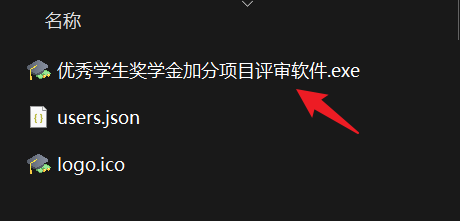
\includegraphics[width=0.3\linewidth]{fig/启动}
		\caption{软件的启动}
		\label{fig:启动}
	\end{figure}
	
	
	正常启动软件后，界面如图\ref{fig:界面}所示。
	\begin{figure}[h]
		\centering
		\small
		
		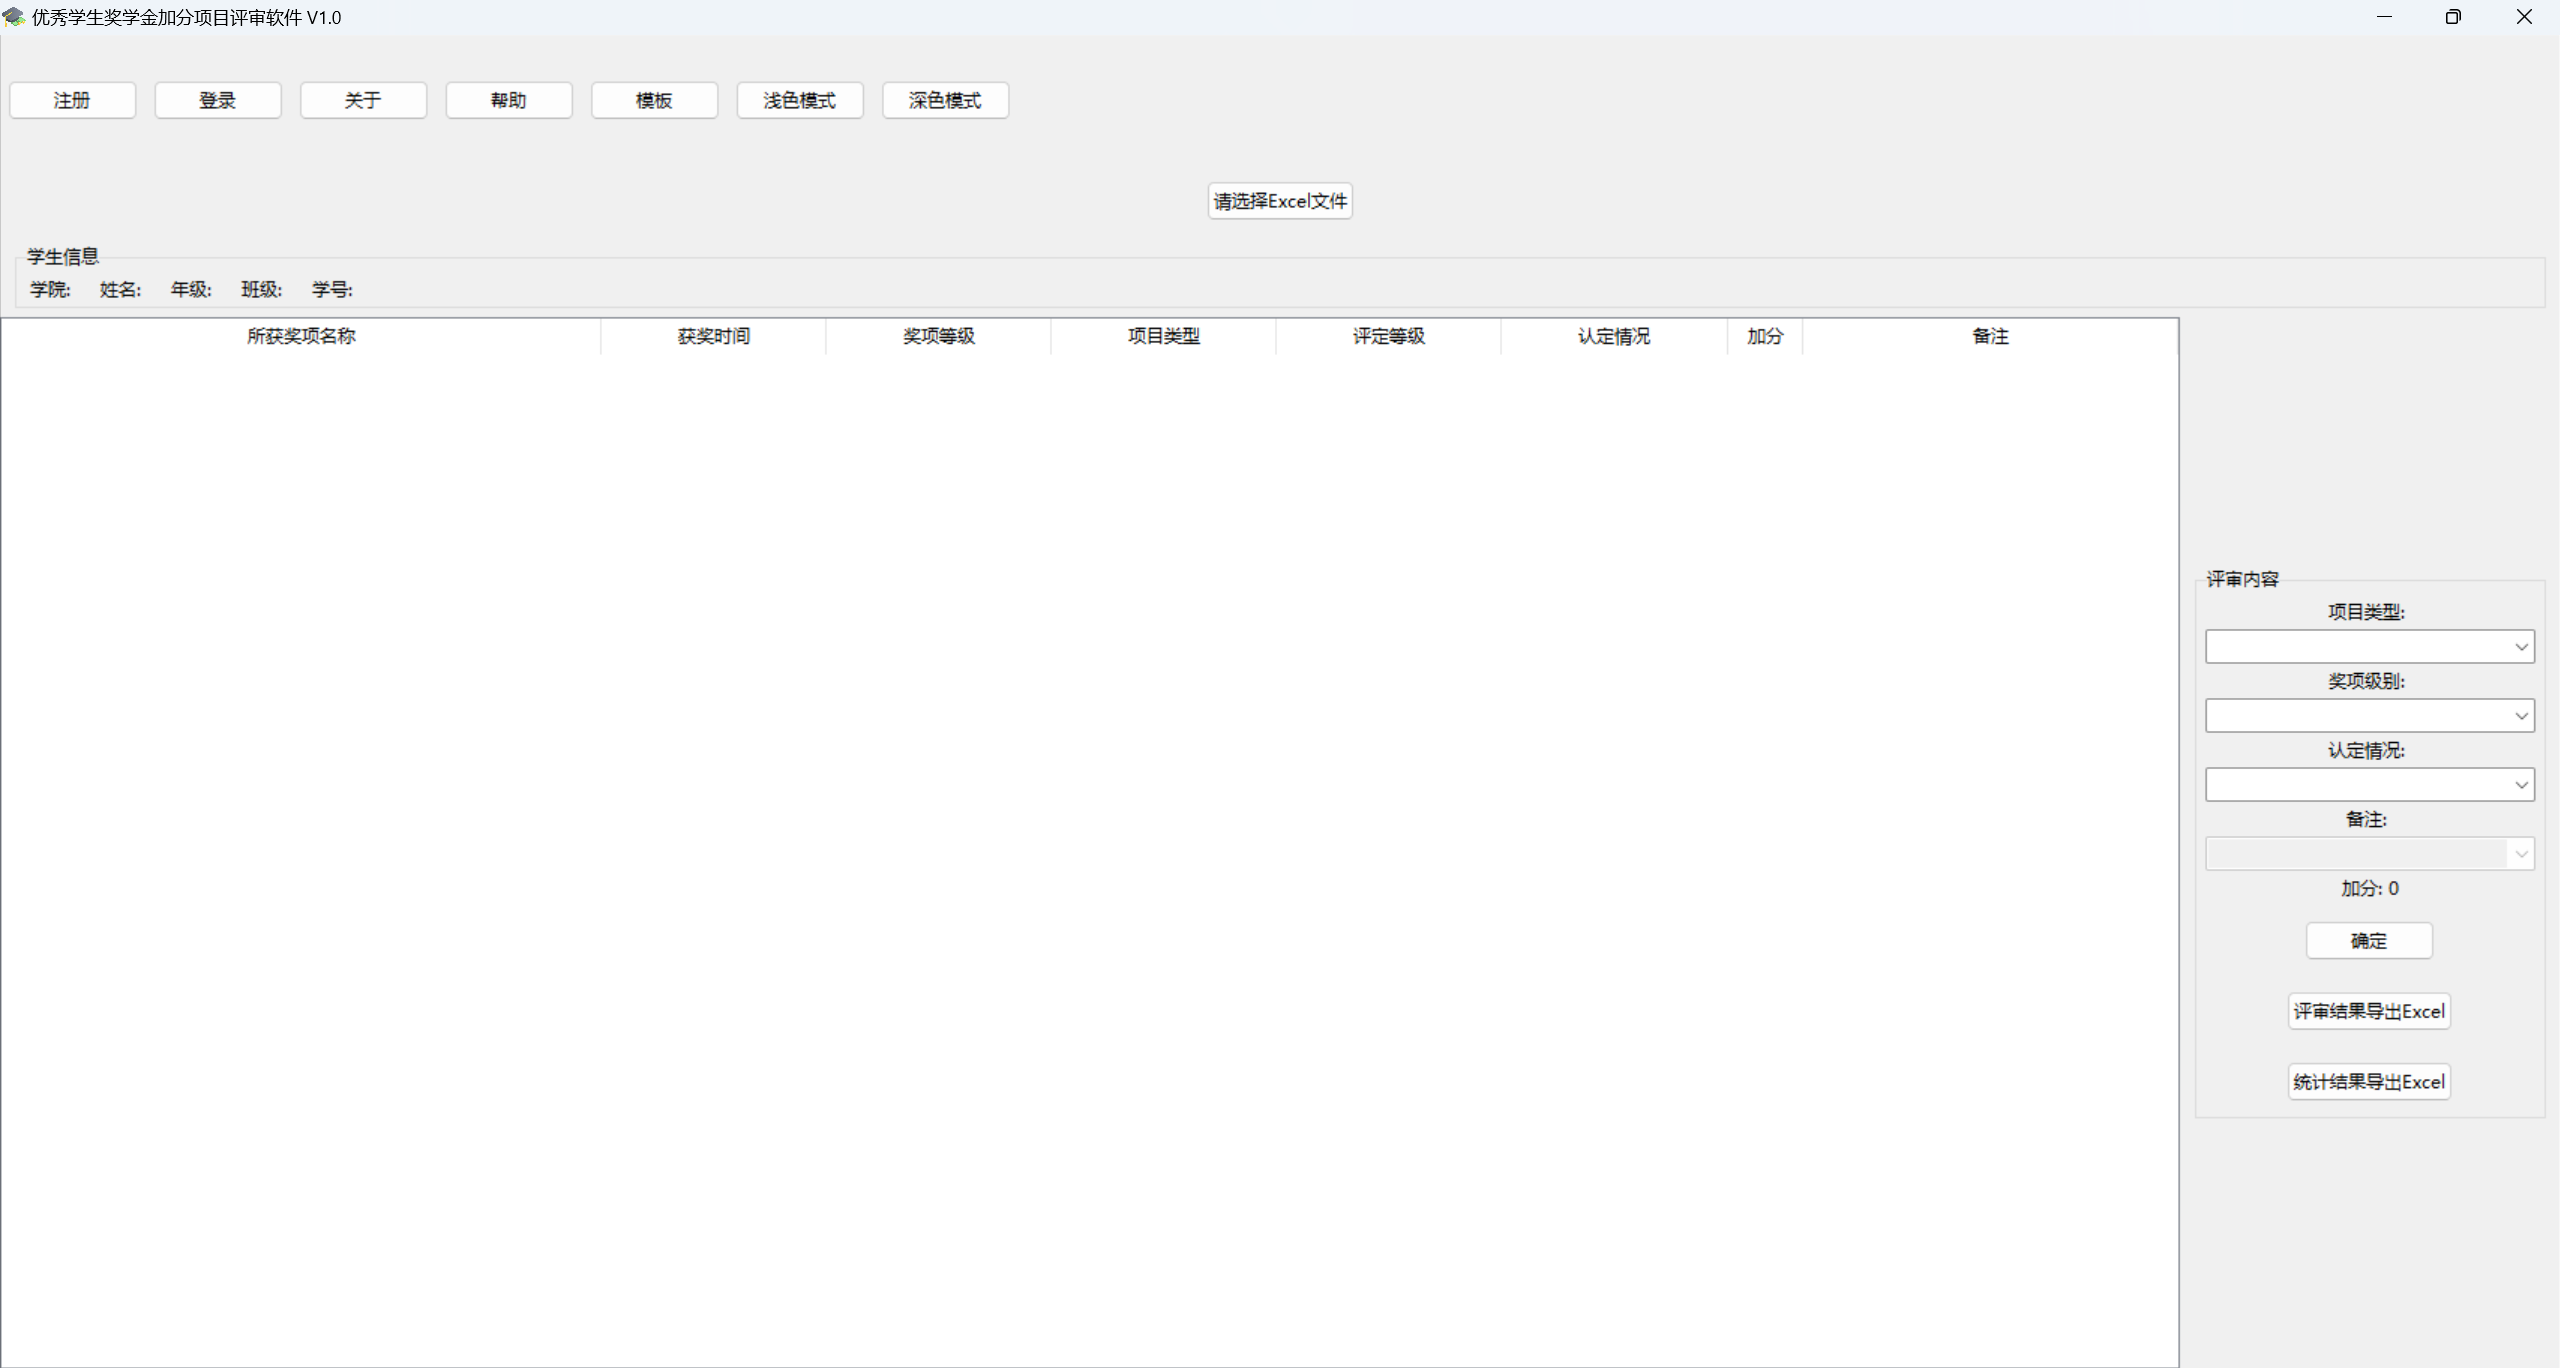
\includegraphics[width=0.5\linewidth]{fig/界面}
		\caption{正常启动的界面}
		\label{fig:界面}
	\end{figure}
	
	
\textcolor{myred}{	
	版本V2.0的启动界面如图\ref{fig:2.0启动界面}所示。
	\begin{figure}[h]
		\centering
		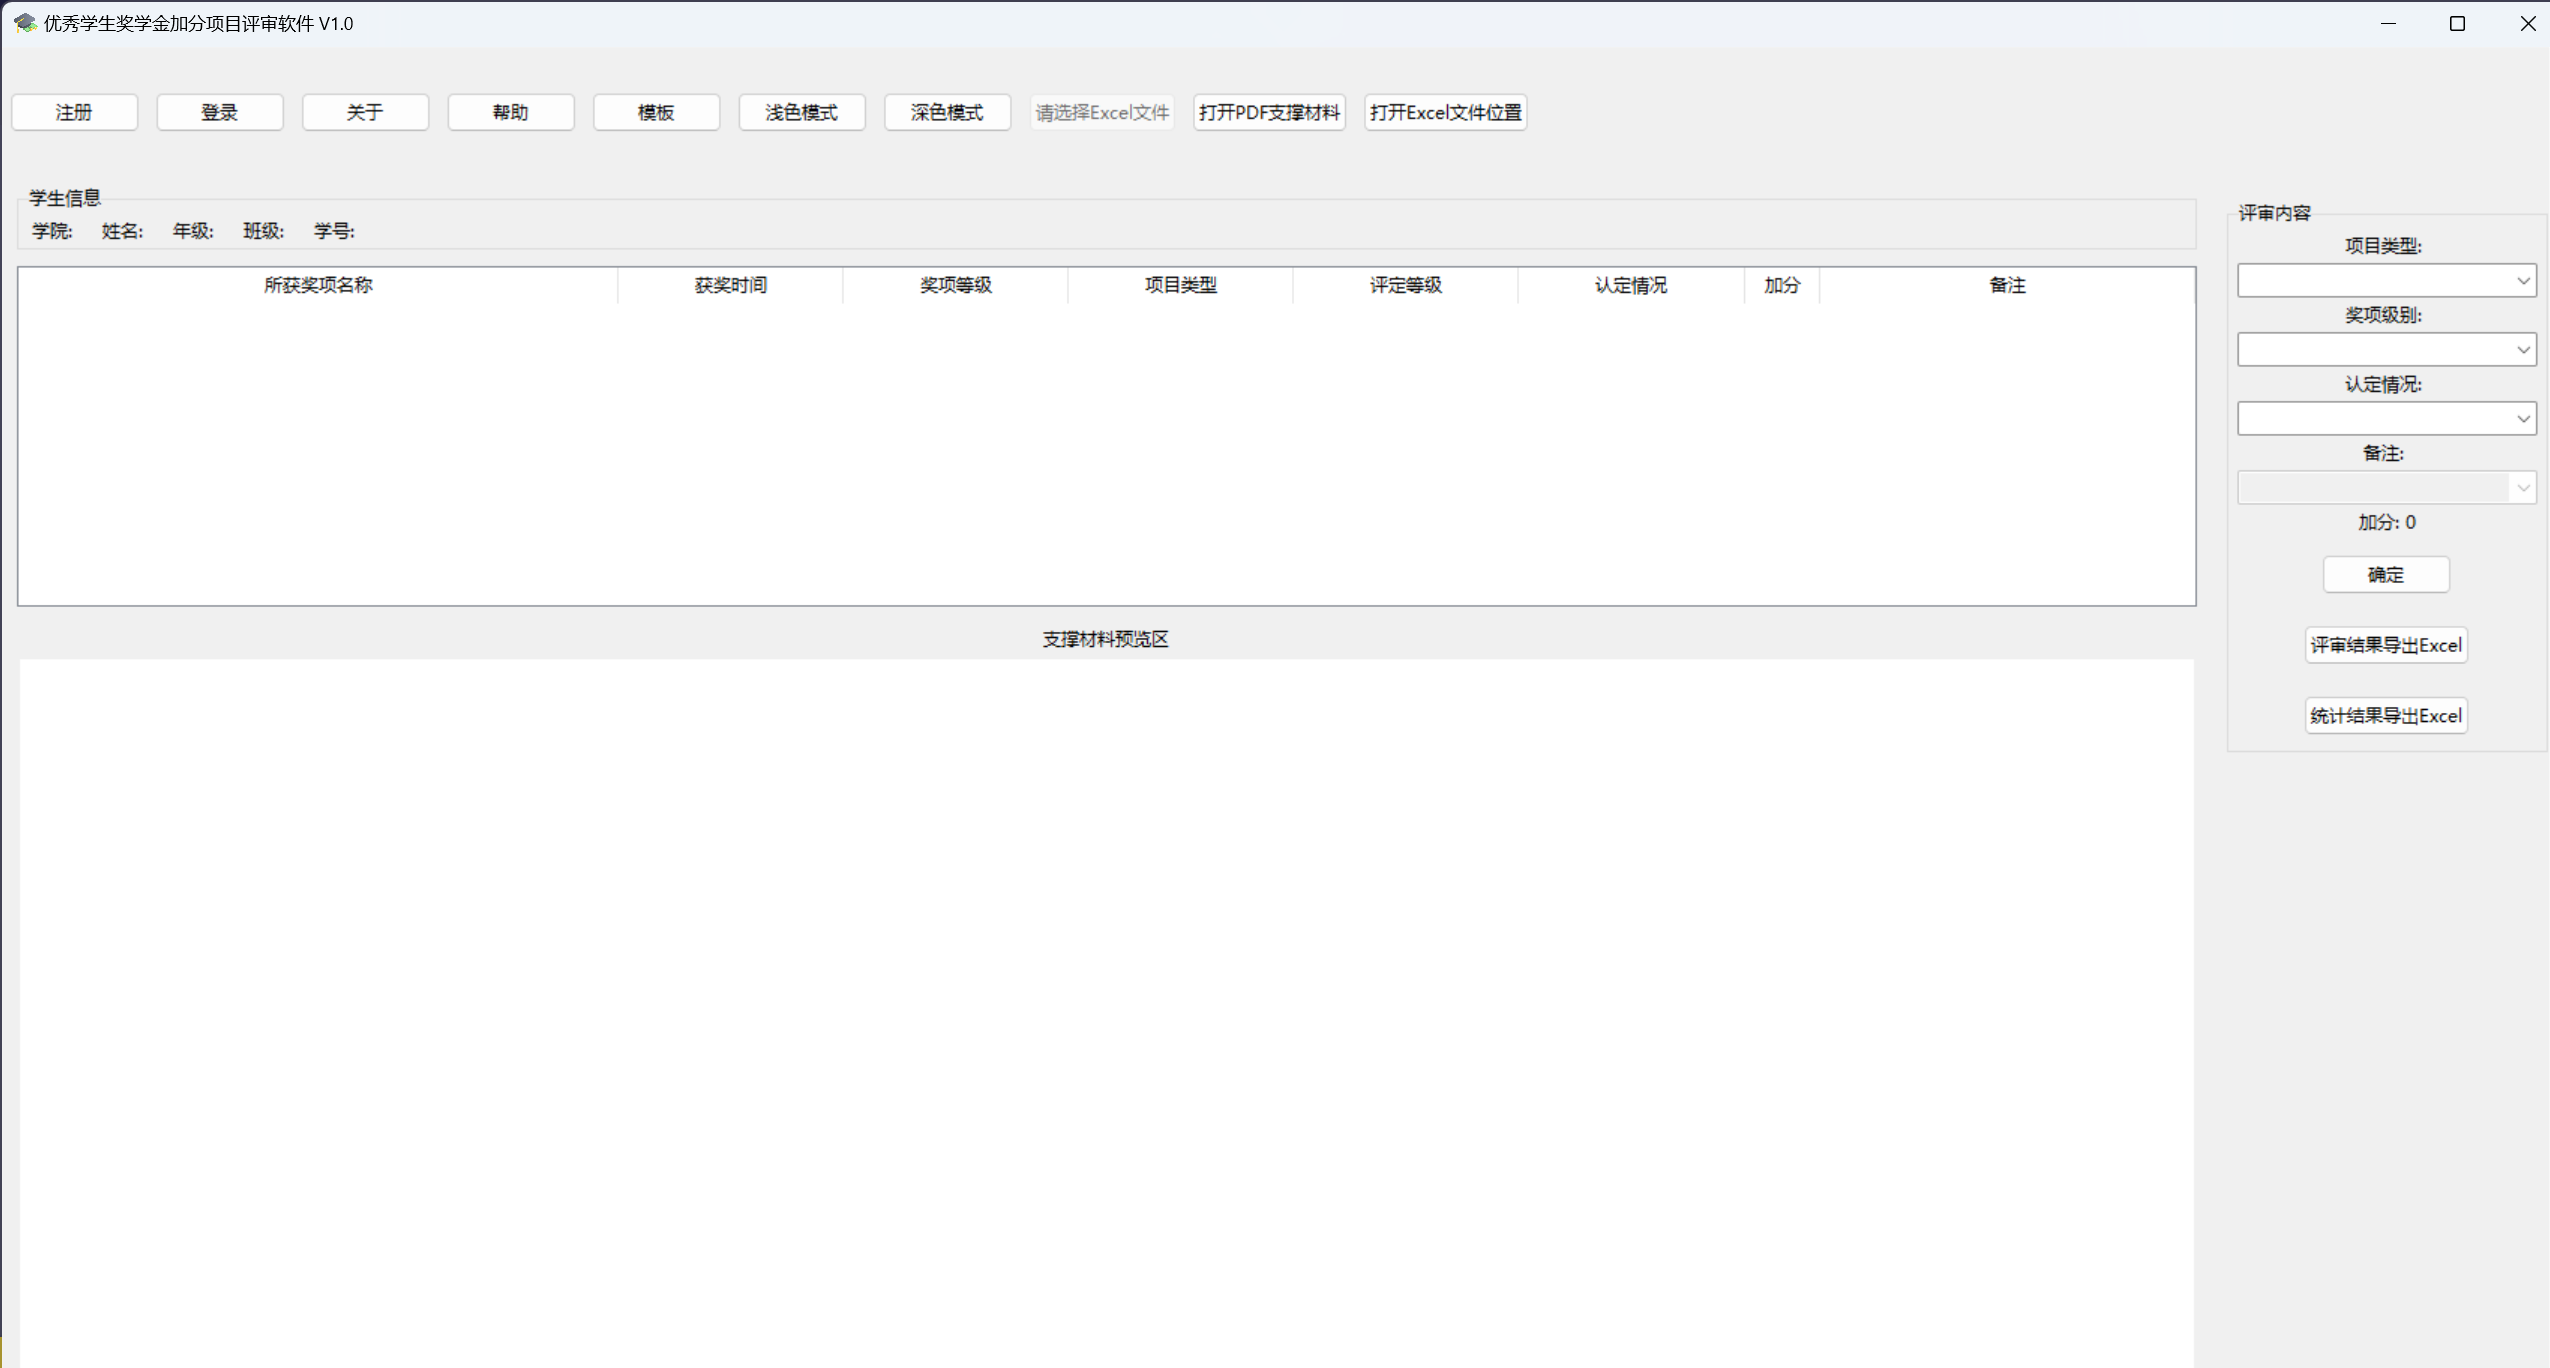
\includegraphics[width=0.7\linewidth]{fig/2.0初始界面}
		\caption{版本V2.0的启动界面}
		\label{fig:2.0启动界面}
	\end{figure}
}

\textcolor{mygreen}{	
	版本V3.0的启动界面如图\ref{fig:3.0启动界面}所示。
	\begin{figure}[h]
		\centering
		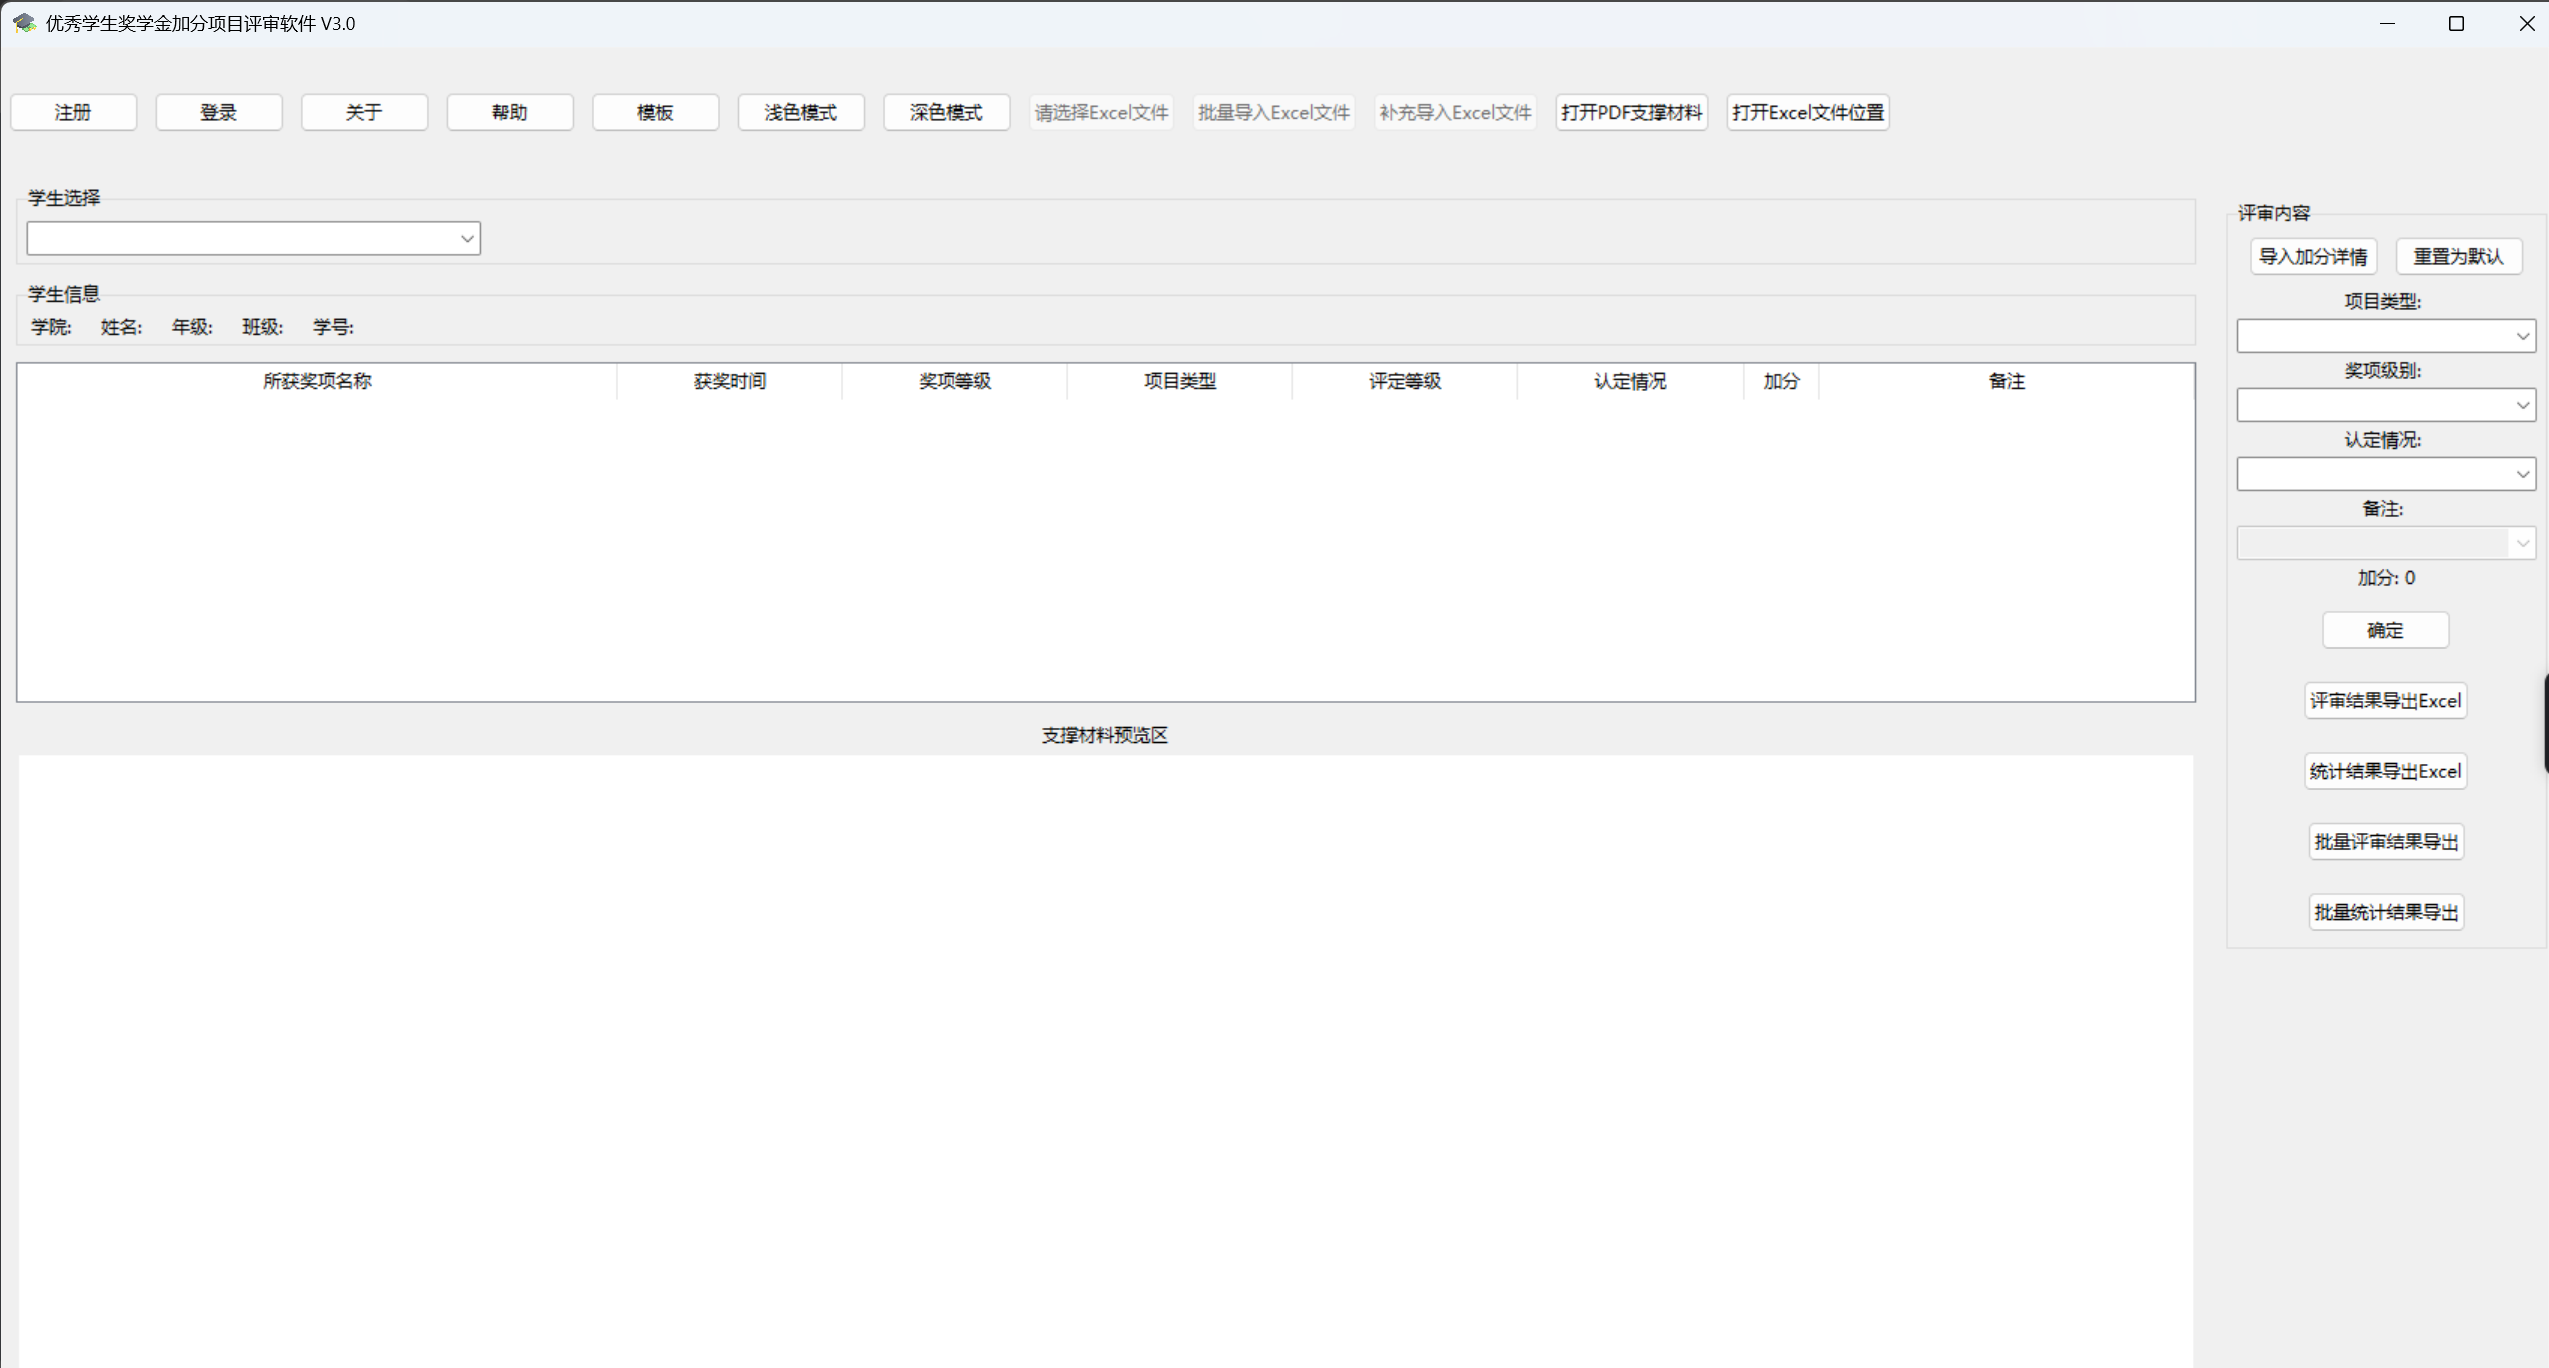
\includegraphics[width=0.7\linewidth]{fig/3.0初始界面}
		\caption{版本V3.0的启动界面}
		\label{fig:3.0启动界面}
	\end{figure}
}

	\section{界面介绍}
	\subsection{导航栏}
	
	如图\ref{fig:导航栏}所示，导航栏位于界面的左上角，共有7个操作按钮，分别是注册、登录、关于、帮助、模板、浅色模式、深色模式（默认启动为浅色模式）。
 
   \textcolor{myred}{
   	版本V2.0的导航栏新添加了“文件导入”按钮，“打开PDF支撑材料”按钮和“打开Excel文件位置”按钮。
   	}
	\begin{figure}[H]
		\centering
		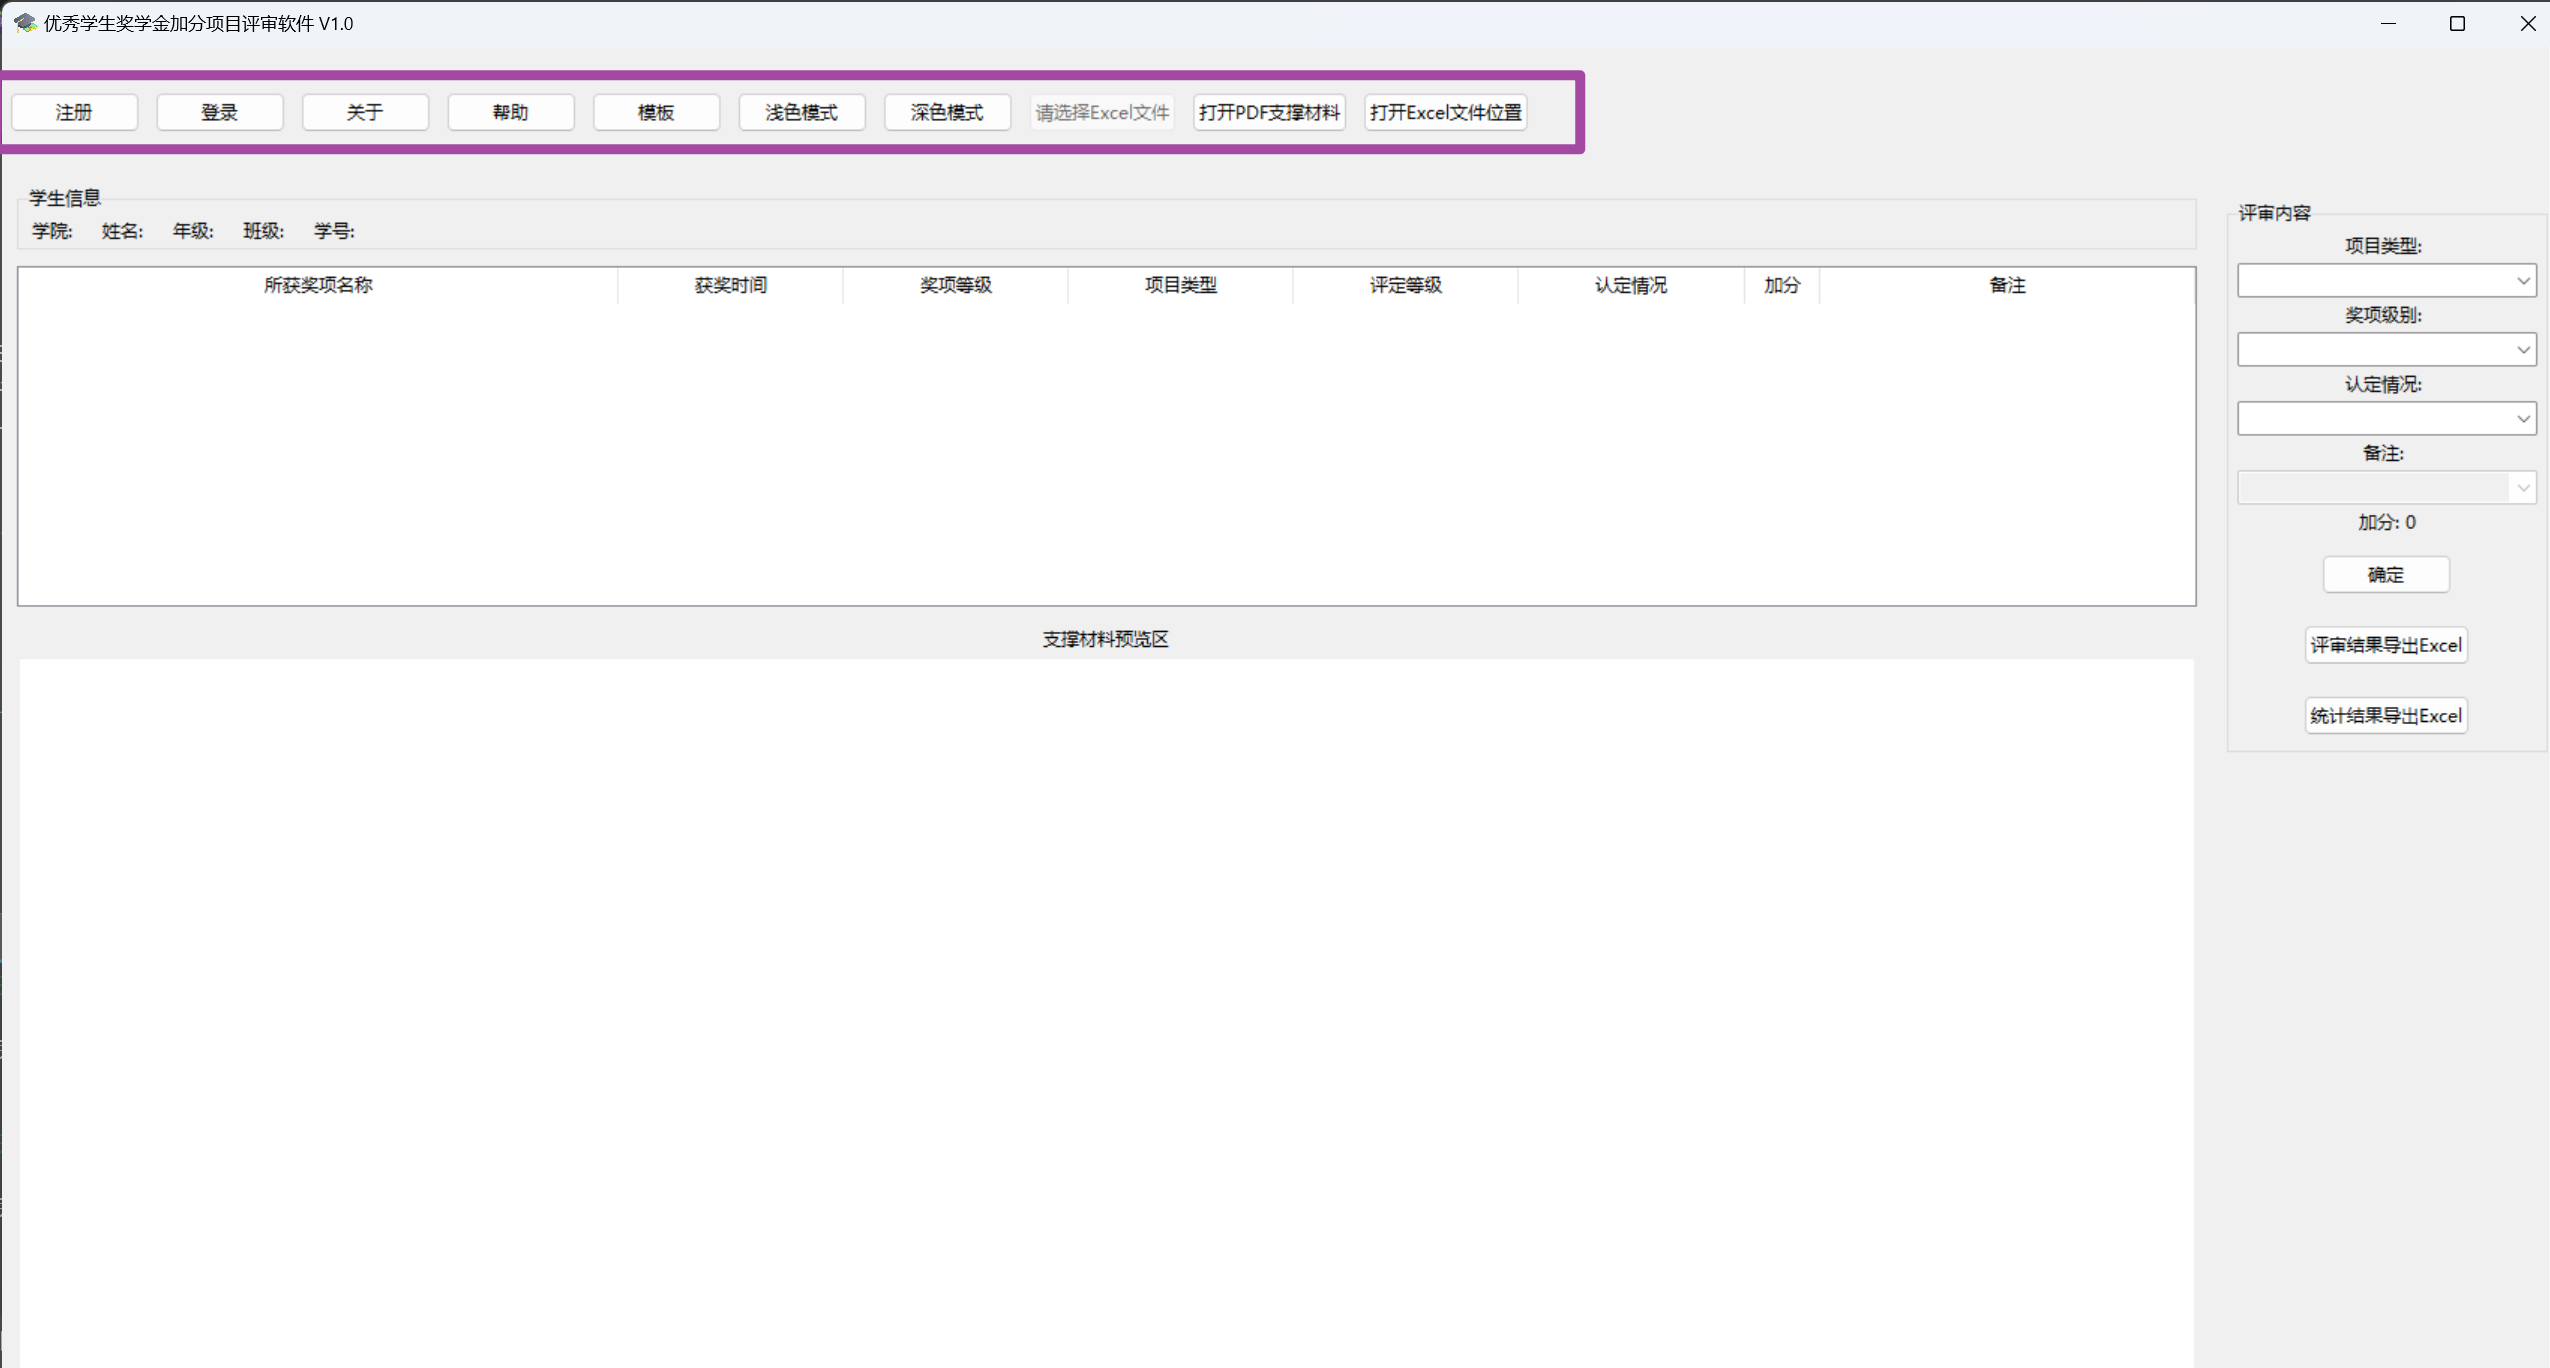
\includegraphics[width=0.7\linewidth]{fig/导航栏}
		\caption{导航栏}
		\label{fig:导航栏}
	\end{figure}
	
	 \textcolor{mygreen}{
		如图\ref{fig:3.0导航栏}所示，版本V3.0的导航栏新添加了“批量导入Excel文件”按钮和“补充导入Excel文件”按钮。
	}
		\begin{figure}[H]
			\centering
			
\includegraphics[width=1\linewidth]{fig/3.0导航条}
			\caption{版本V3.0的导航栏}
			\label{fig:3.0导航栏}
	\end{figure}
	
	\subsection{文件导入按钮}
	
	如图\ref{fig:导入文件}所示，文件导入按钮“请选择Excel文件”位于界面的较上方的中间位置，点击后即可选取对应的Excel.xlsx文件导入。
	\begin{figure}[H]
		\centering
		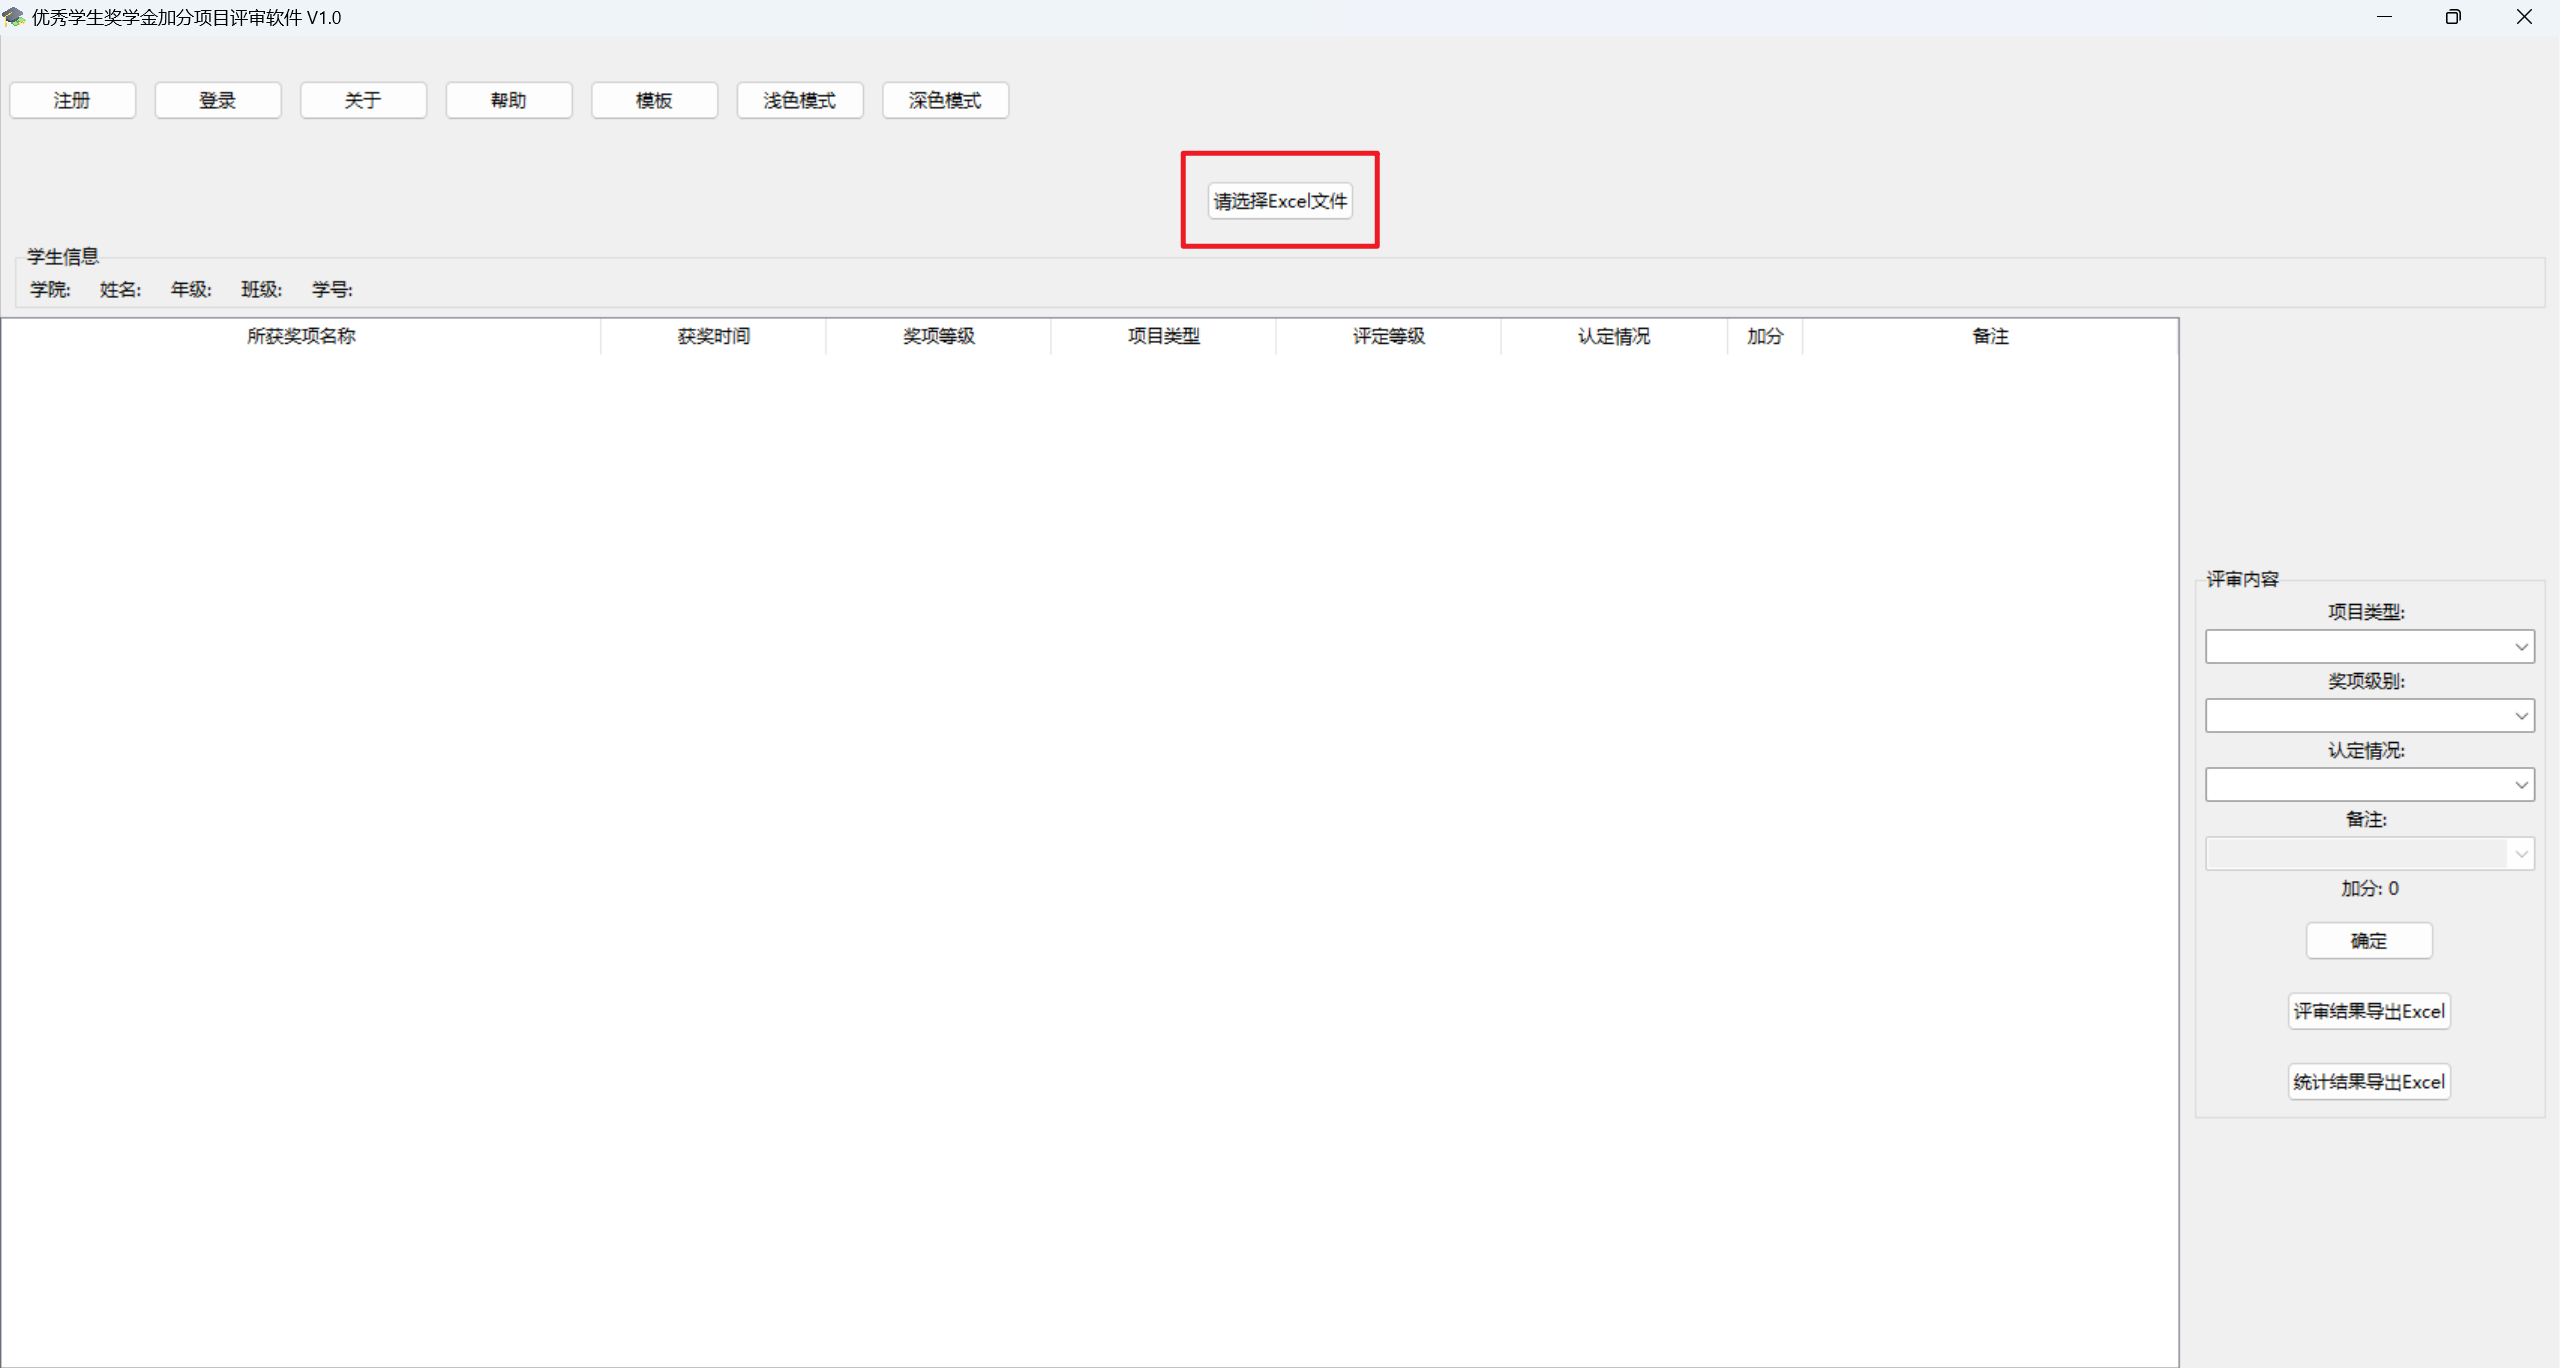
\includegraphics[width=0.7\linewidth]{fig/导入文件}
		\caption{文件导入按钮}
		\label{fig:导入文件}
	\end{figure}
	
	
\textcolor{myred}{
		如图\ref{fig:2.0文件导入}所示，版本V2.0的文件导入按钮更新到了导航栏中，并且默认为暗色（不要可点选），只有登录后才可点选。
	\begin{figure}[H]
		\centering
		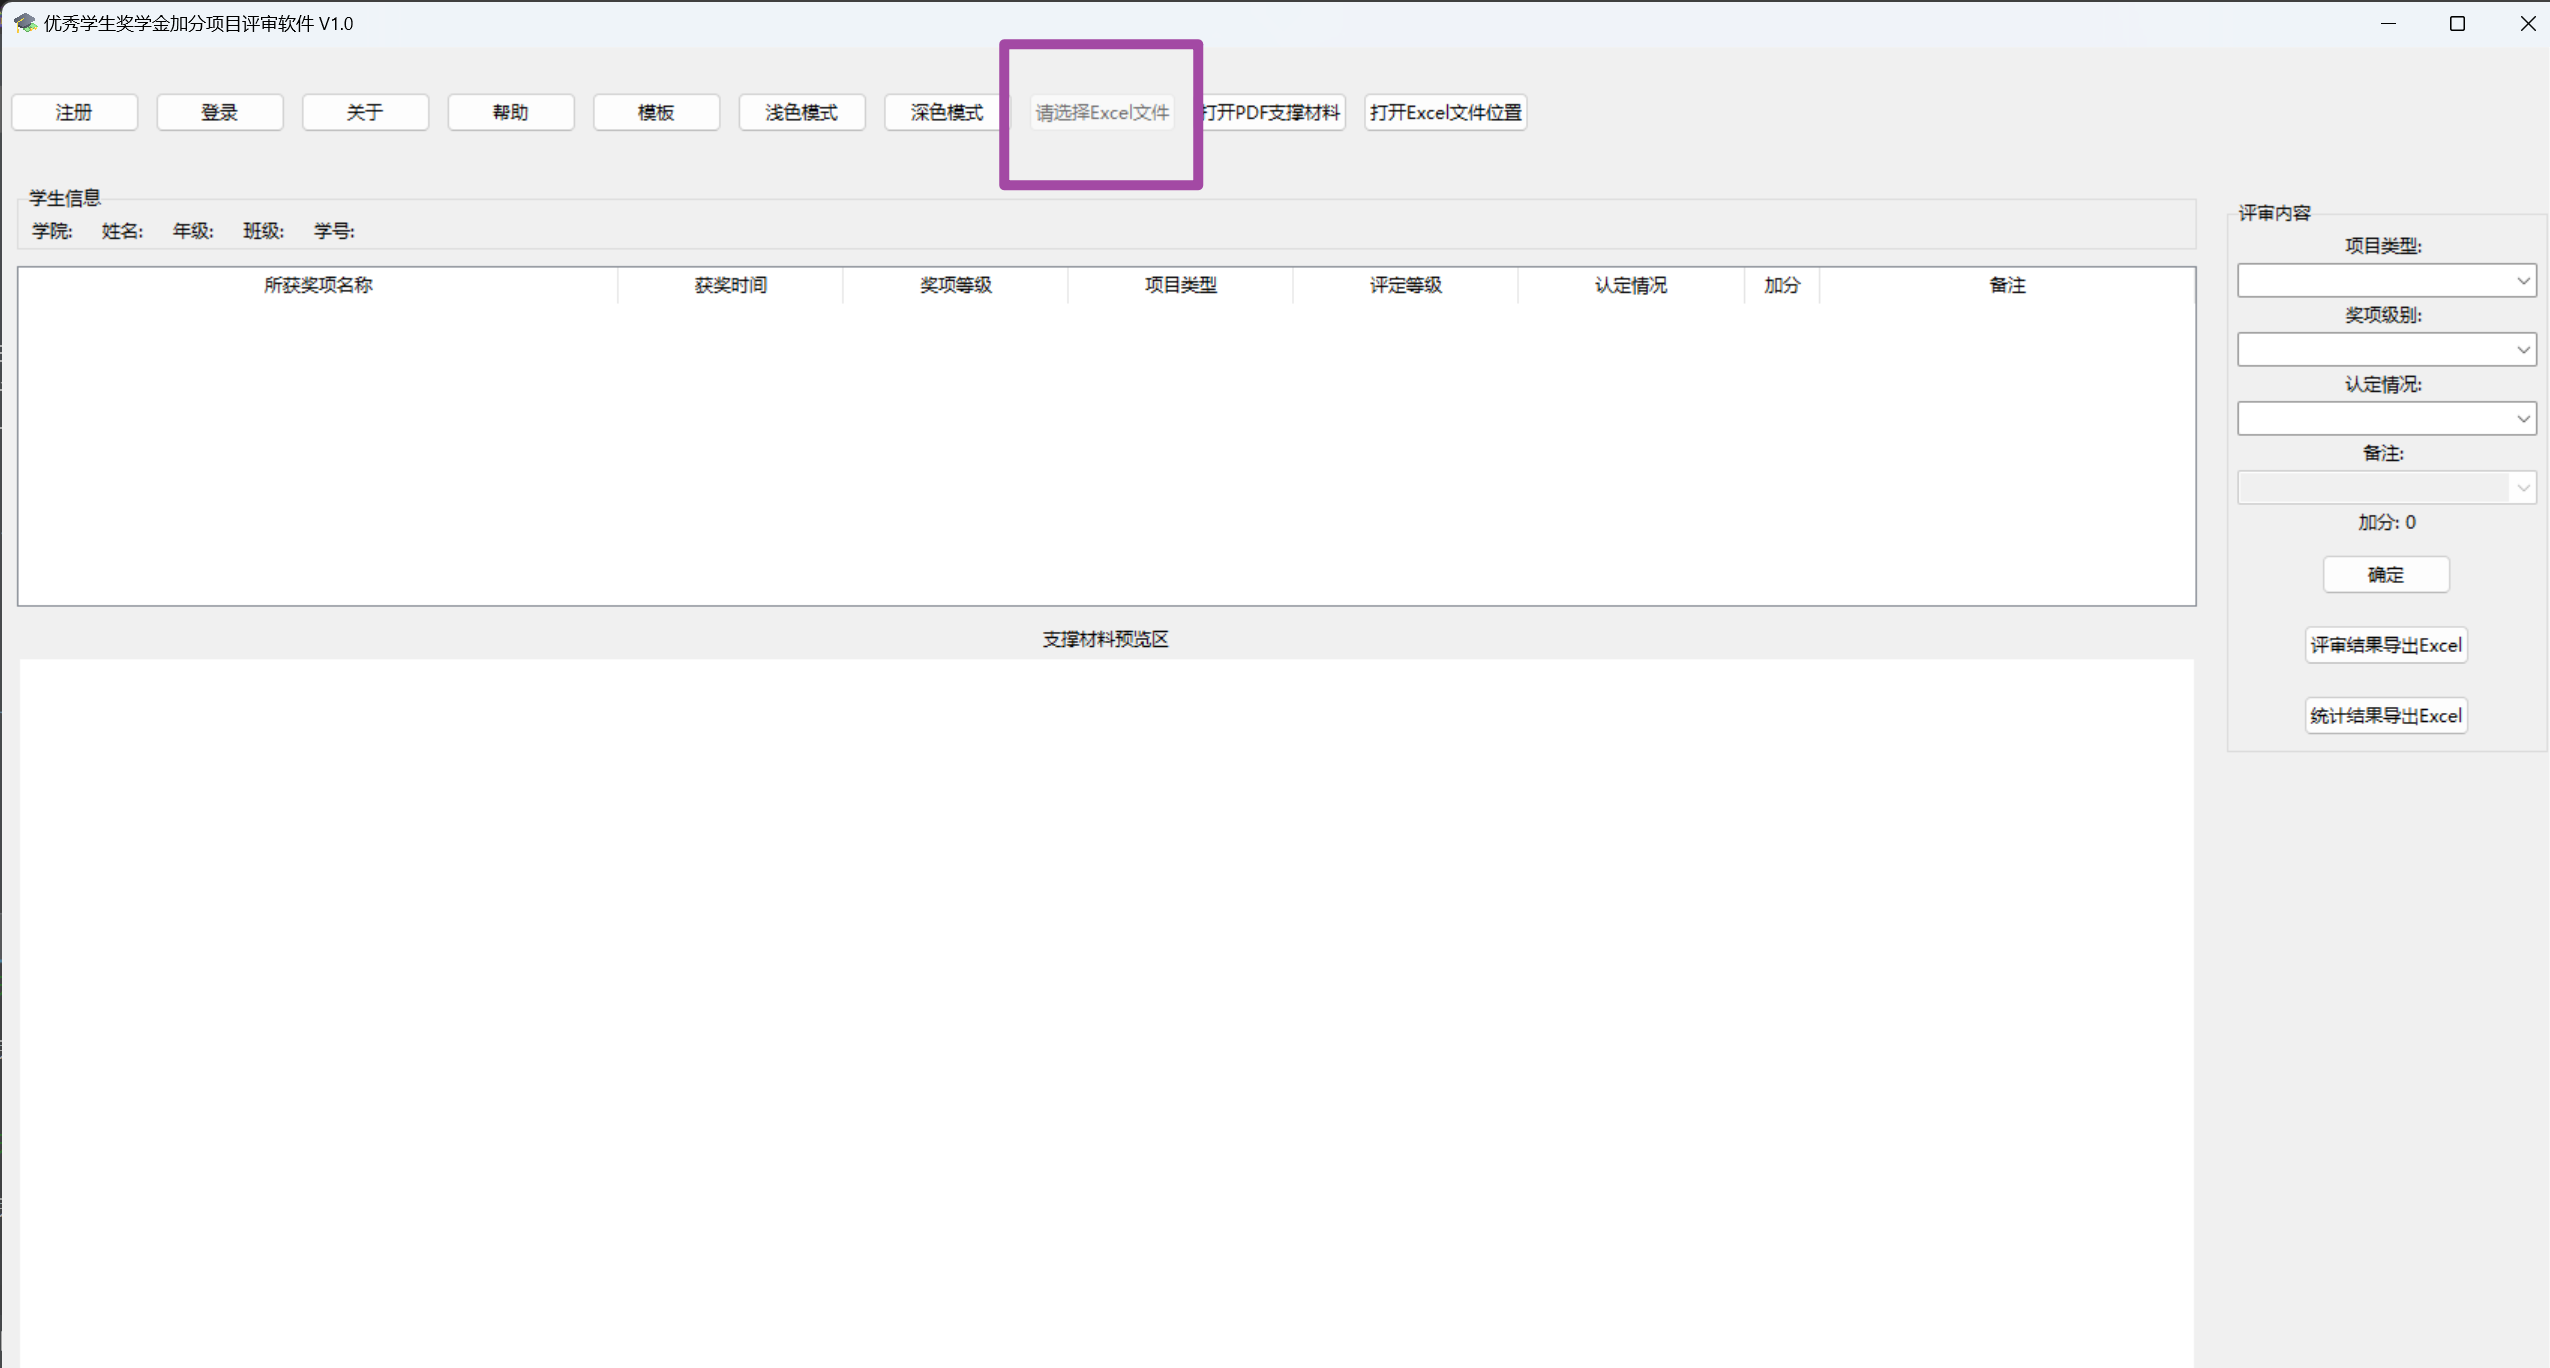
\includegraphics[width=0.7\linewidth]{fig/2.0文件导入}
		\caption{版本V2.0的文件导入按钮}
		\label{fig:2.0文件导入}
	\end{figure}
}
	
	\textcolor{mygreen}{
	如图\ref{fig:3.0导航栏}所示，版本V3.0支持“批量导入Excel文件”和“补充导入Excel文件”这两个文件导入功能，两个功能按钮默认为暗色（不要可点选），只有登录后才可点选。}
	

	
	\subsection{评审界面}
	
	如图\ref{fig:评审界面}所示，评审界面位于界面的中间位置，其分为三个片区，红框为读取导入文件后的学生信息，包括学院、姓名、年级、班级、学号；绿框为读取导入文件后的加分项目信息，包括所获奖项名称、获奖时间、奖项等级、项目类型、评定等级、认定情况、加分、备注；蓝框为读取评审人的评审操作按钮，包括对项目类型、奖项级别、认定情况、备注的下拉选择菜单，评审“确定”按钮，以及评审结果导出和统计结果导出两个按钮。
	\begin{figure}[h]
		\centering
		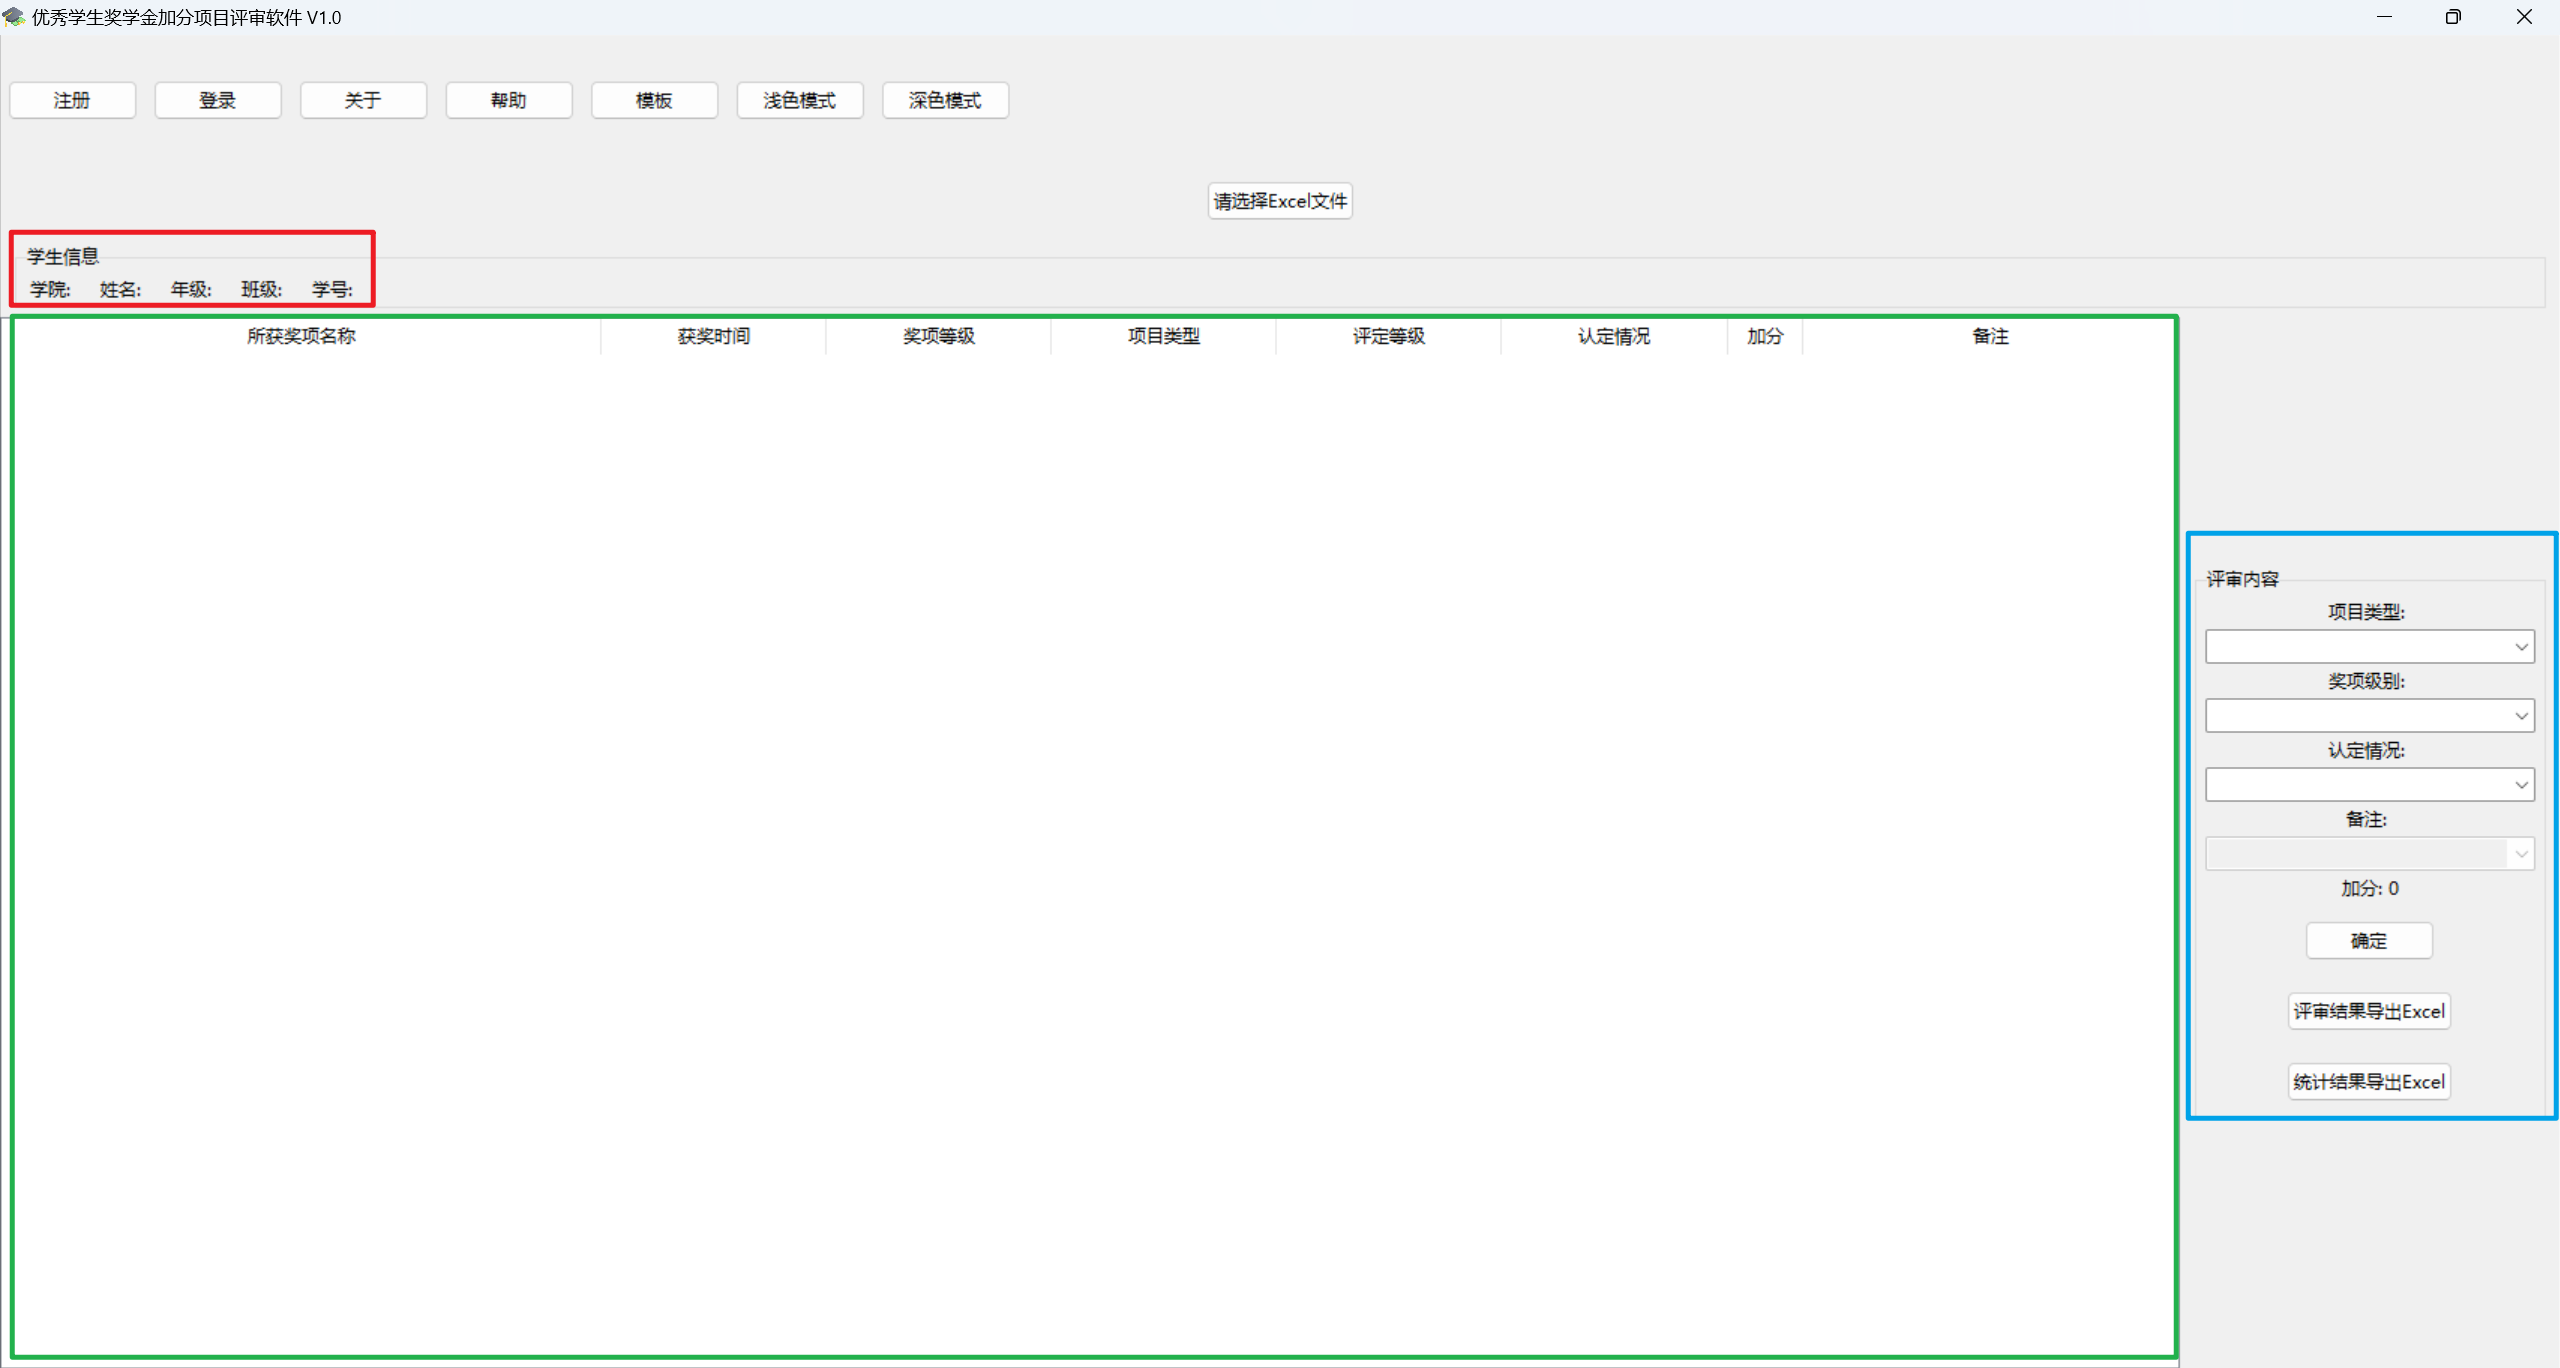
\includegraphics[width=0.7\linewidth]{fig/评审界面}
		\caption{评审界面}
		\label{fig:评审界面}
	\end{figure}
	
	\textcolor{mygreen}{
	如图\ref{fig:版本V3.0评审界面新功能按钮展示}所示，为版本V3.0的评审界面，在学生信息的上方新增加了“学生选择”下拉菜单；在评审内容区域，新增加了“导入加分详情”按钮、“重置为默认”按钮、“批量评审结果导出”按钮、“批量统计结果导出”按钮，其各自功能将在后续章节内容进行阐述。
	}
	\begin{figure}[h]
		\centering
		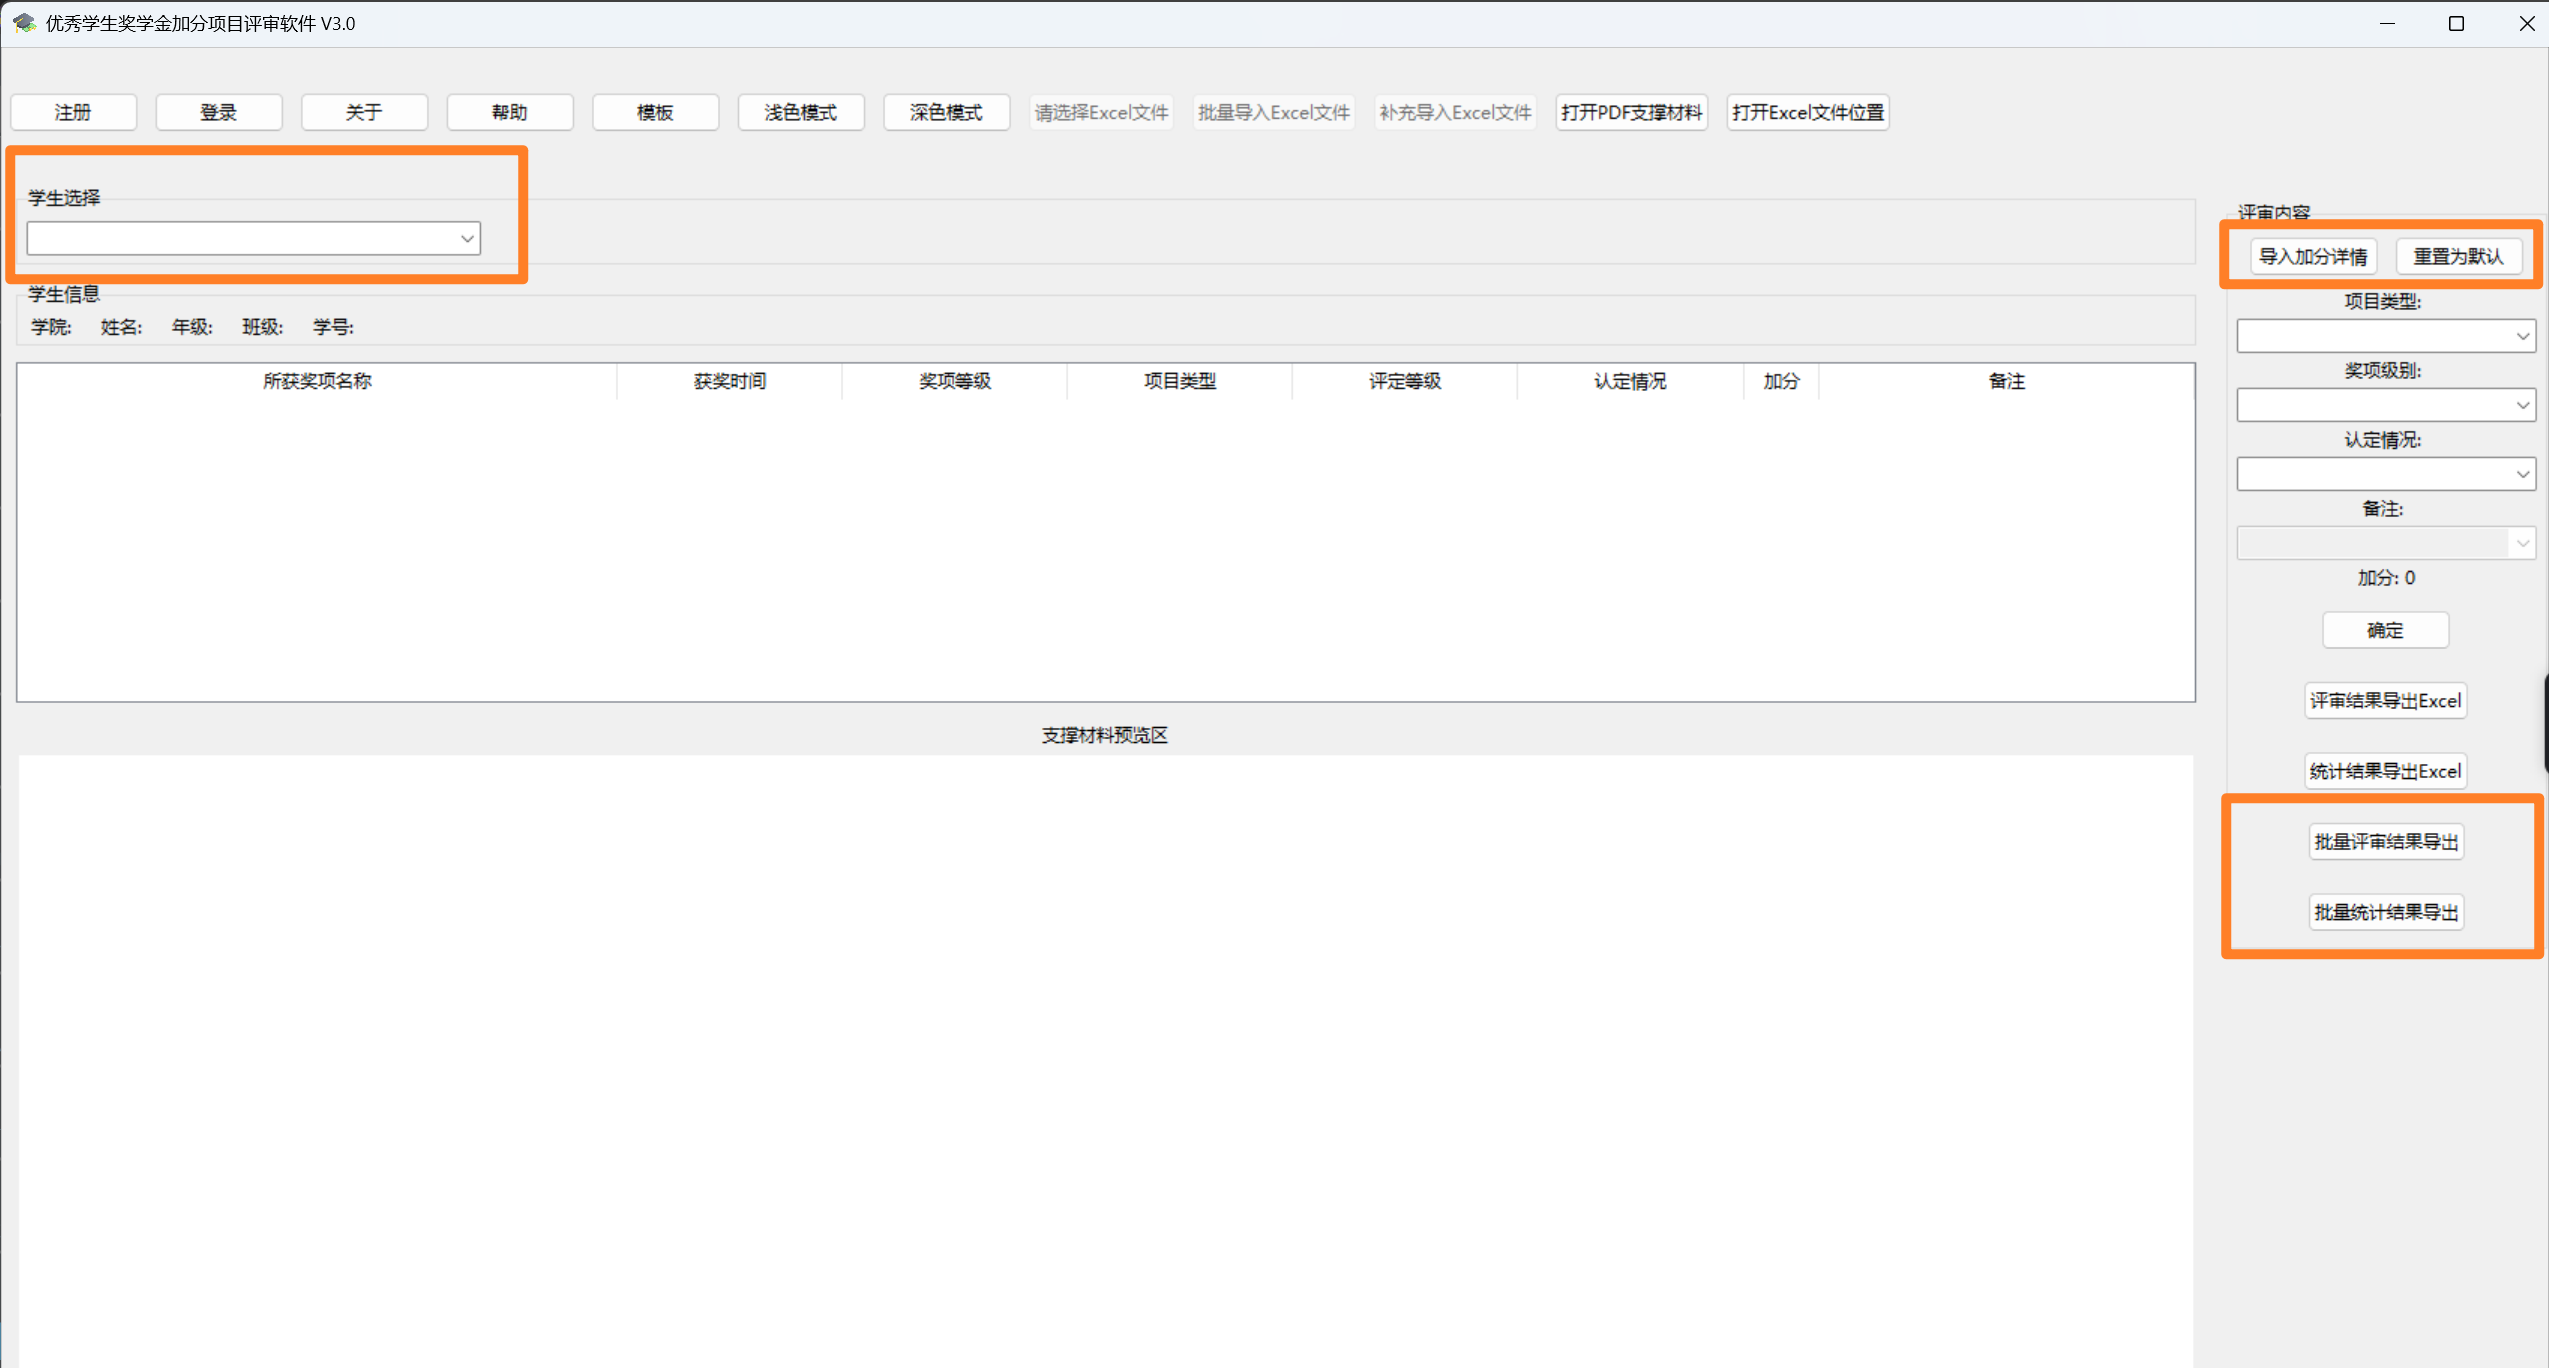
\includegraphics[width=0.7\linewidth]{fig/3.0评审界面新功能}
		\caption{版本V3.0评审界面新功能按钮展示}
		\label{fig:版本V3.0评审界面新功能按钮展示}
	\end{figure}
	
	
	
\textcolor{myred}{
	\subsection{支撑材料预览区}
	如图\ref{fig:支撑材料预览区}所示，为版本V2.0添加的支撑材料预览区，可以显示导入的EXCEL文件的同一目录下的与“所获奖项名称”相同的文件名的图片（jpg、jpeg和png格式），如果文件为pdf文件，则会提示点击“打开PDF支撑材料”按钮进行打开。
	\begin{figure}[H]
		\centering
		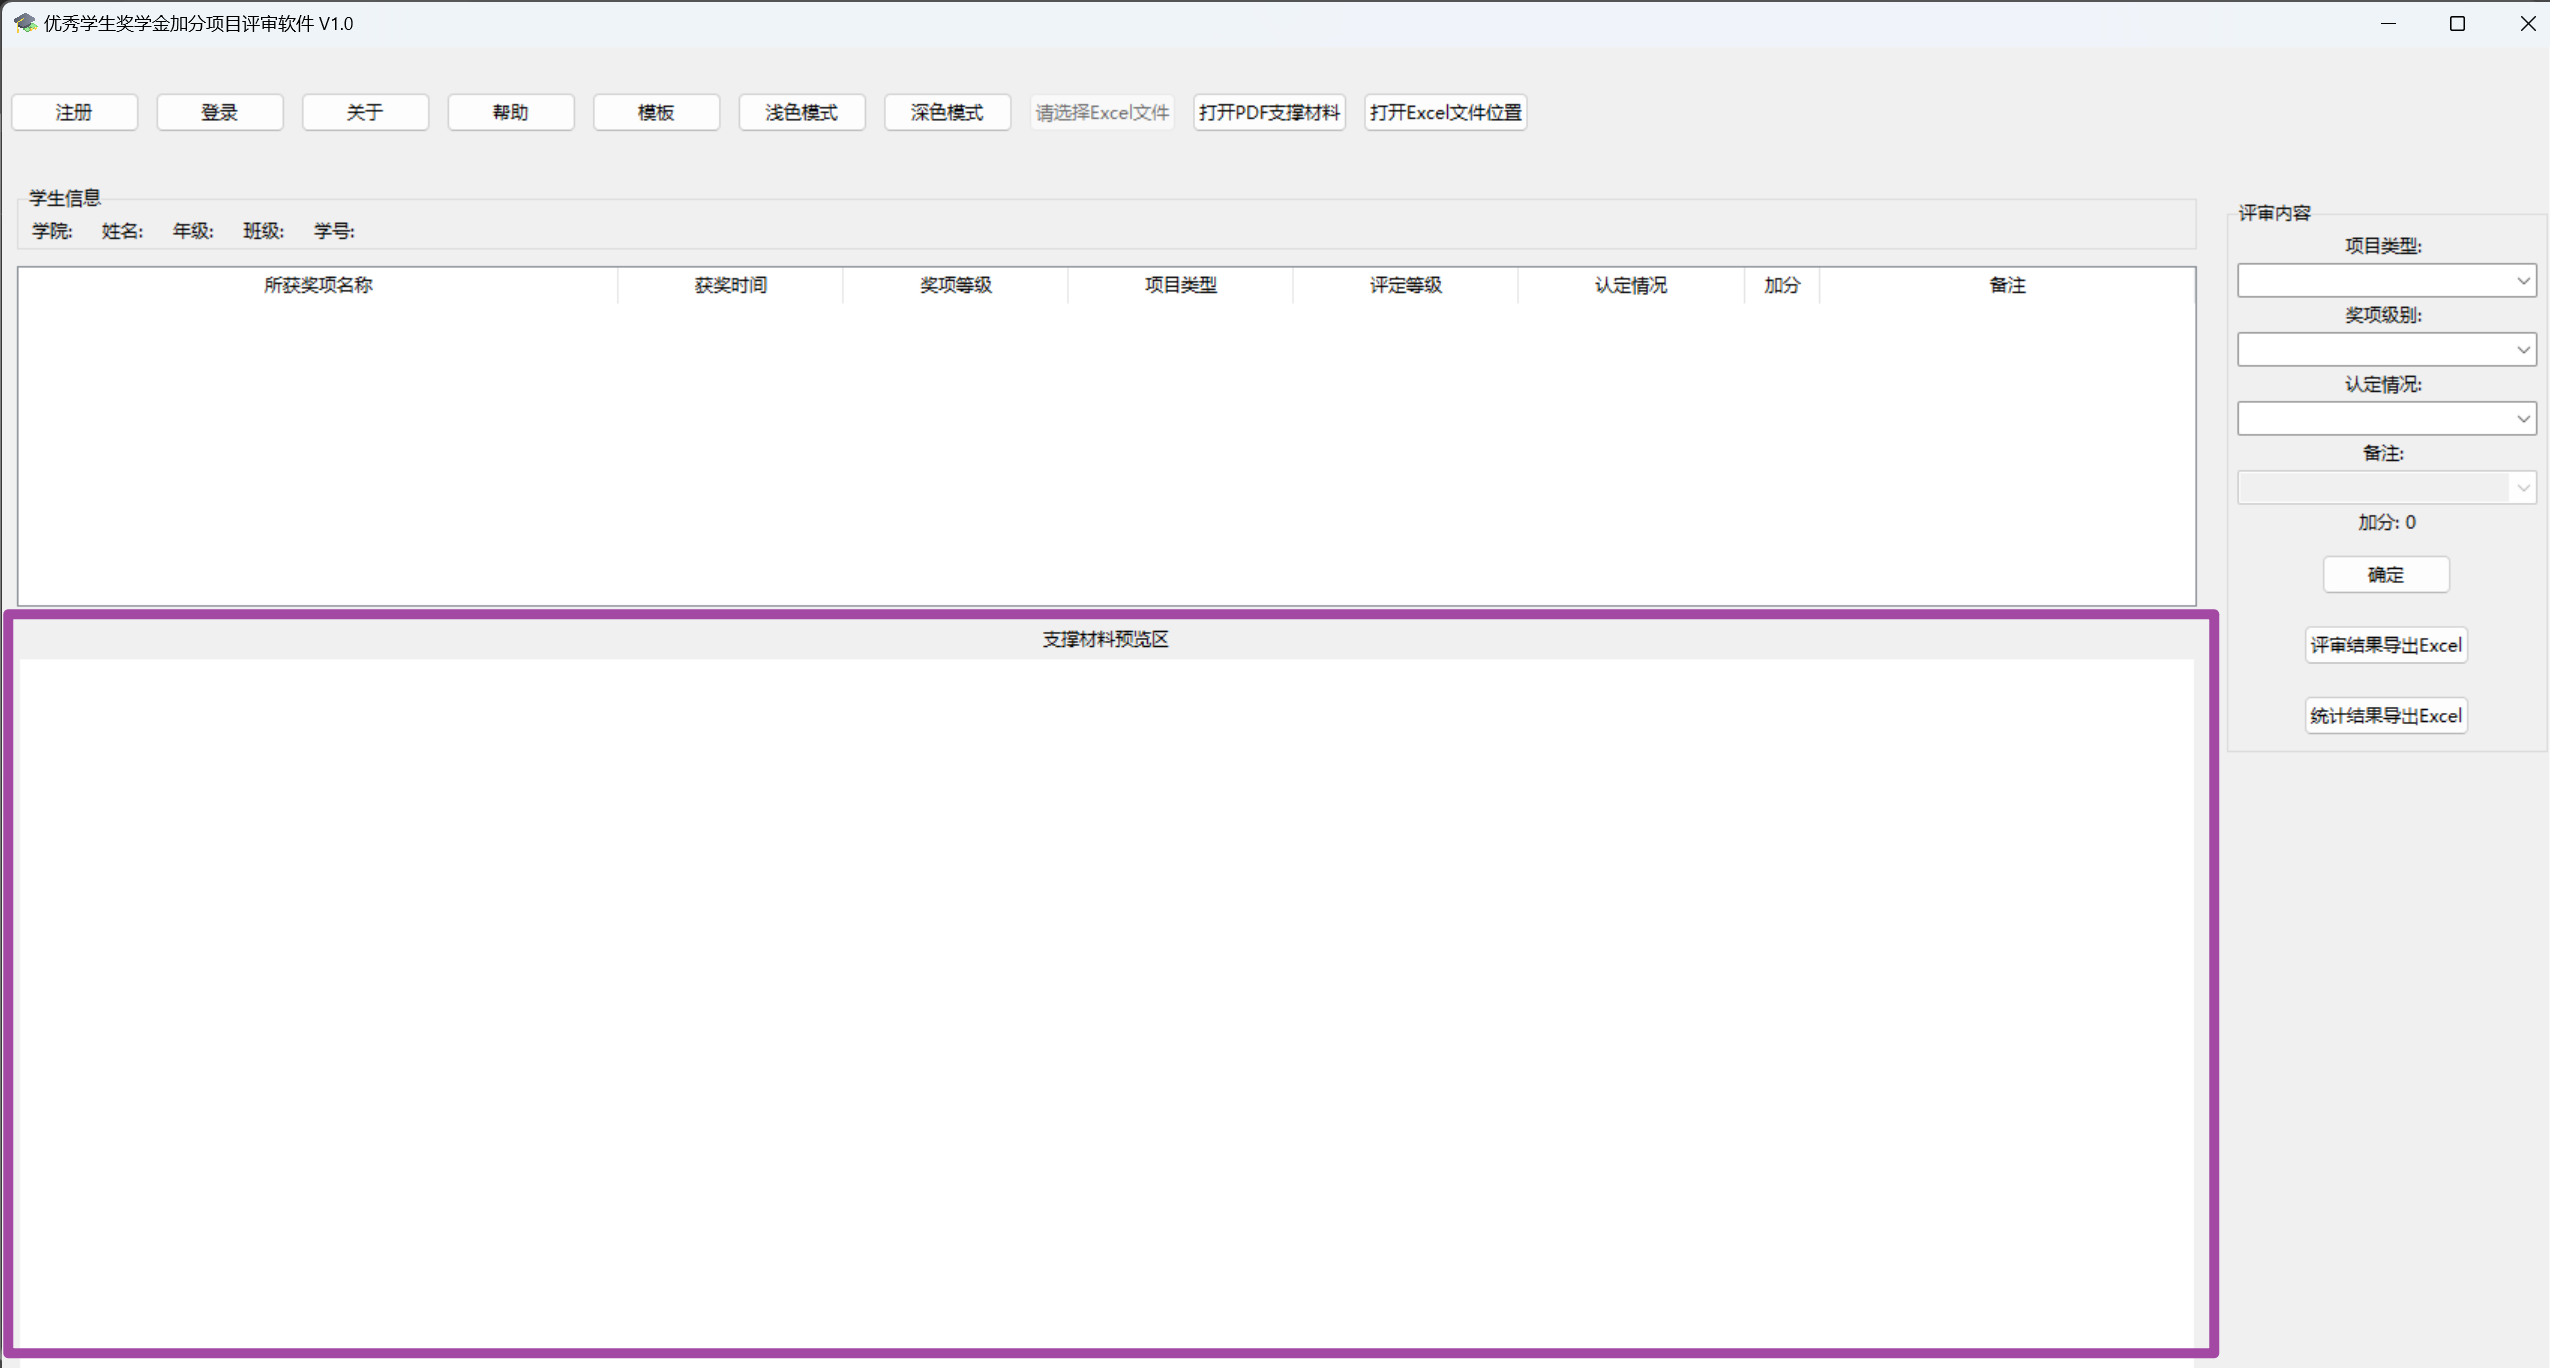
\includegraphics[width=0.7\linewidth]{fig/支撑材料预览区}
		\caption{支撑材料预览区}
		\label{fig:支撑材料预览区}
	\end{figure}
}	
	\newpage
	\chapter{软件操作教程}
	\section{评审基本流程概述}
	
	如图\ref{fig:基本流程图}所示，为本软件的基本使用流程图，其中绿框内容为前期准备工作，由申请加分项目人员完成；蓝框内容为评审工作，由评审人员（即本软件用户）完成。
	\begin{figure}[H]
		\centering
		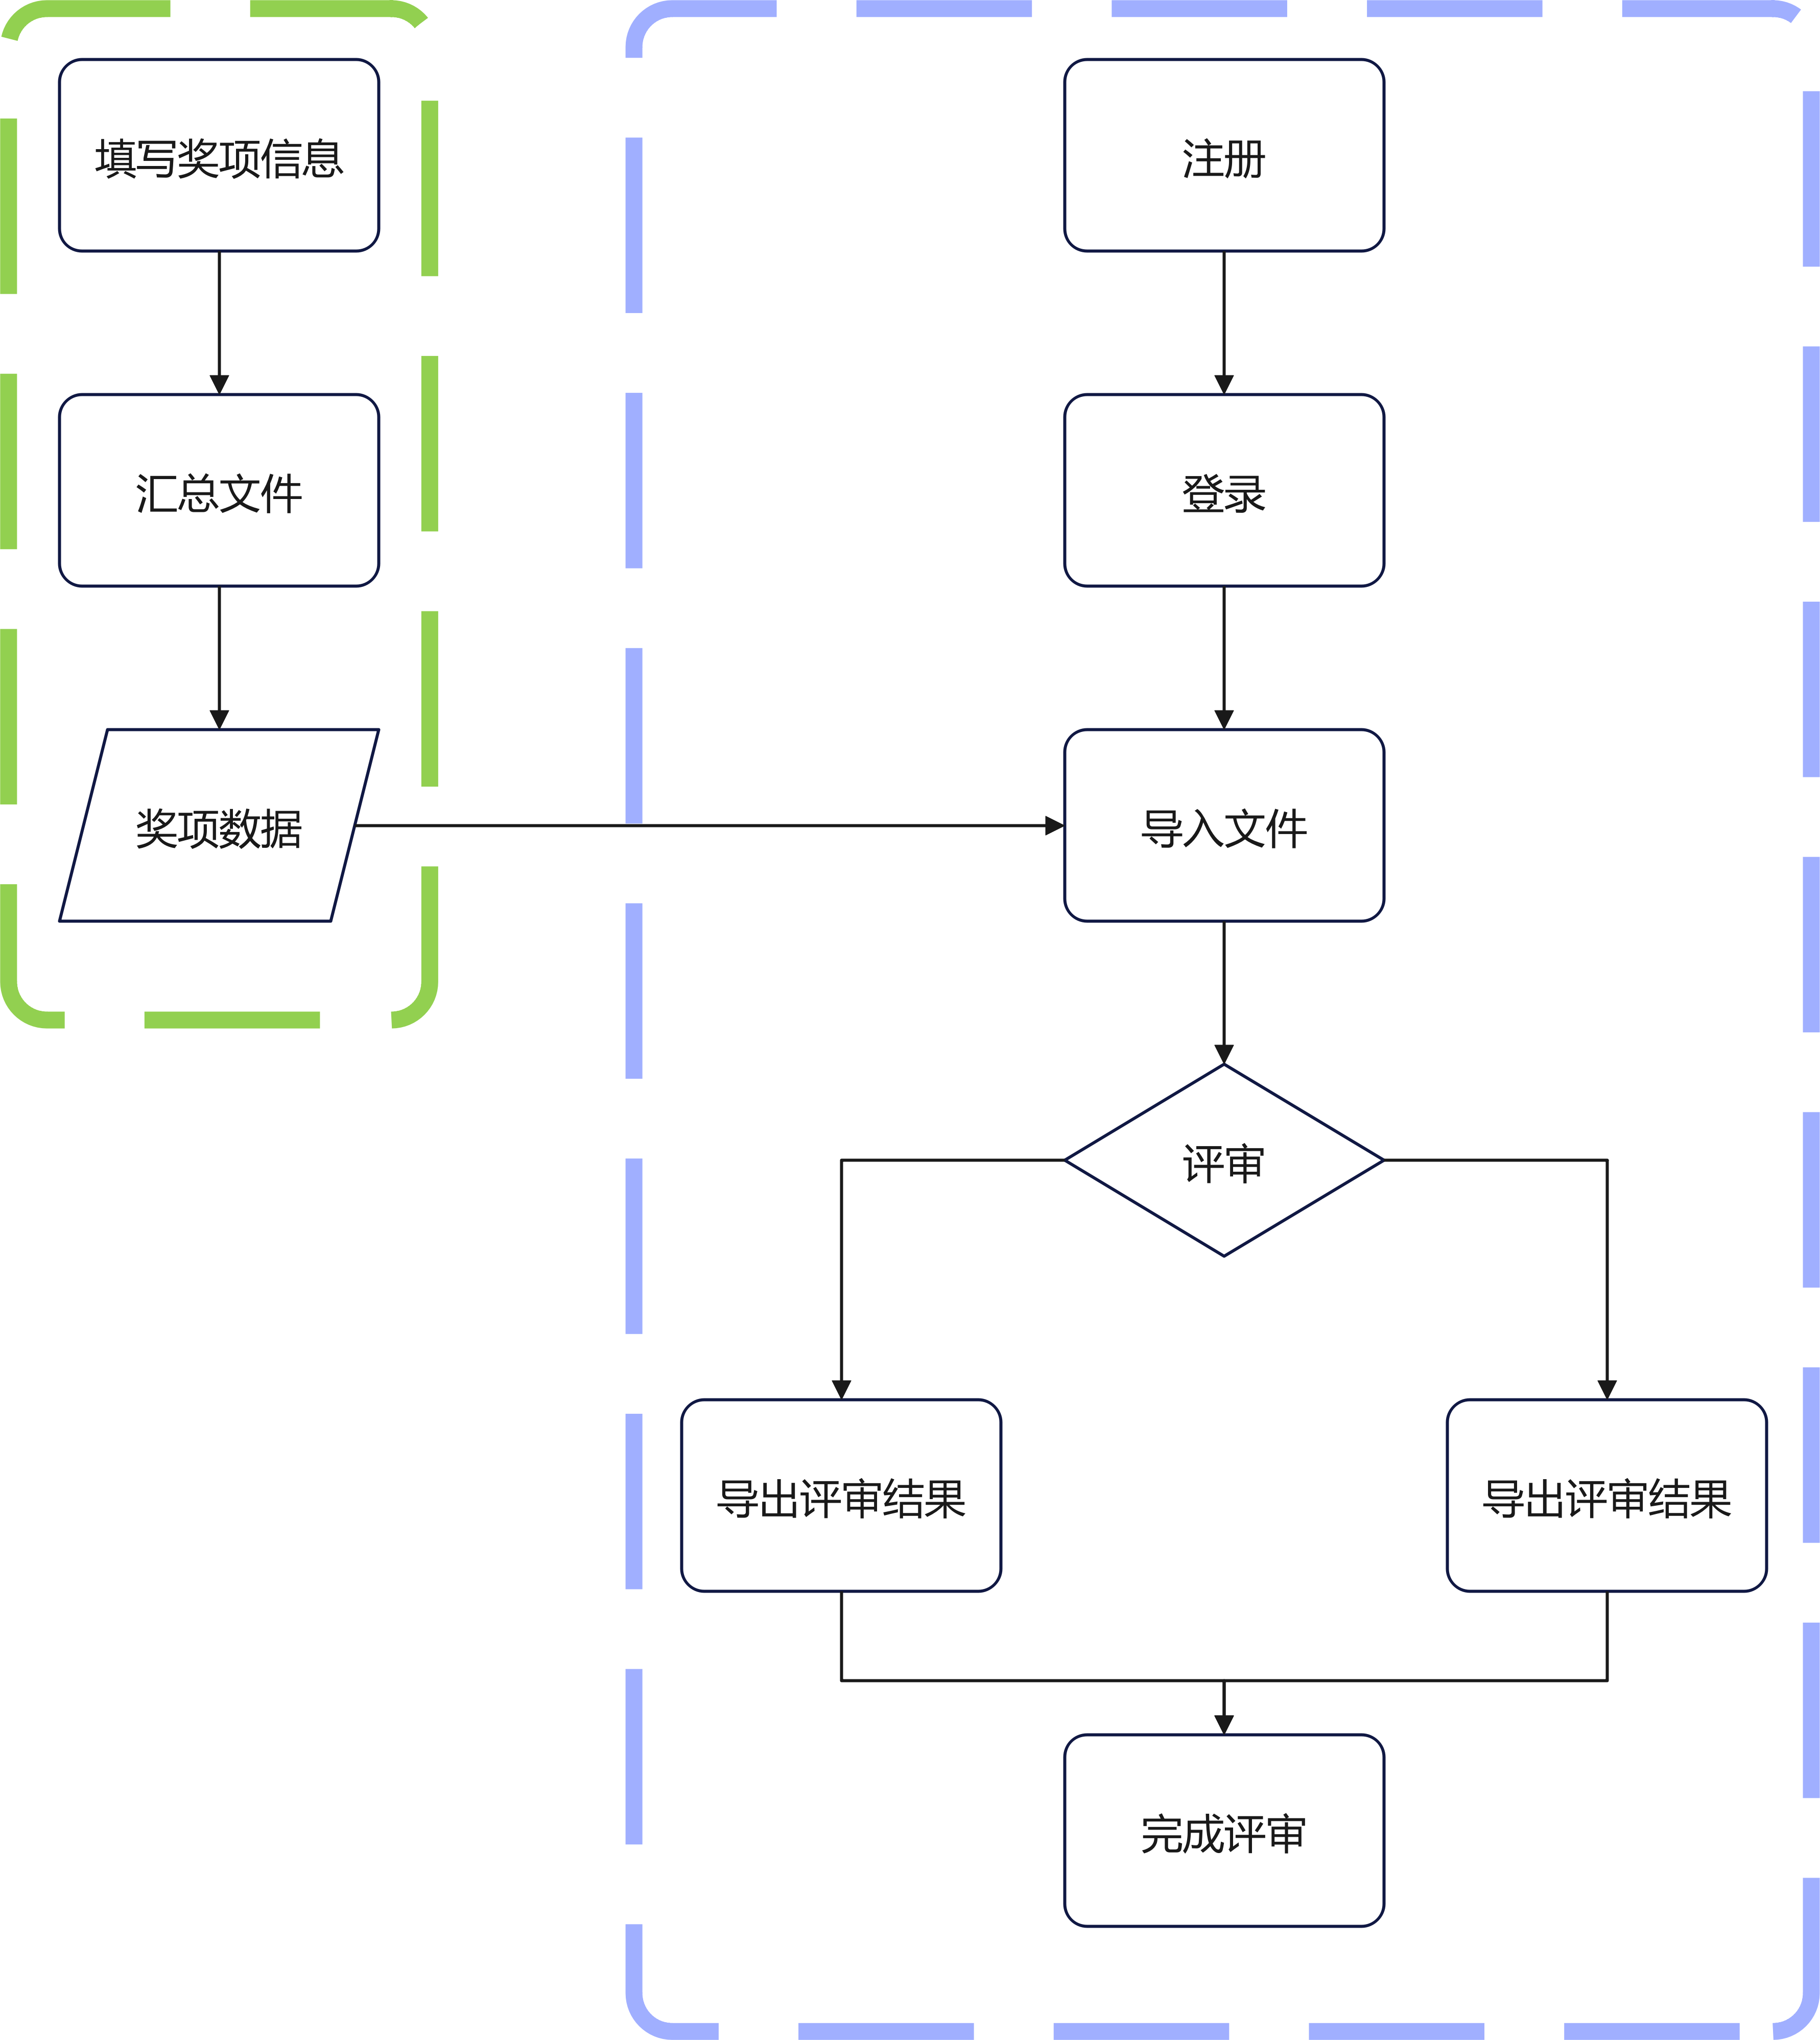
\includegraphics[width=0.6\linewidth]{fig/基本流程图}
		\caption{基本流程图}
		\label{fig:基本流程图}
	\end{figure}
	
	\section{前期准备工作}
	\subsection{加分项目信息的数据收集}
	
	在进行优秀学生奖学金加分项目审核前，需收集申请加分项目人员的基本信息以及加分项目的信息，包括学院，姓名，年级，班级，学号，所获奖项名称，获奖时间，奖项等级，项目类型。
	
	为了提供用户更好的使用体验，在本软件的导航栏中设置有收集模板文件，如图\ref{fig:模板文件的下载}所示，点击后会弹窗显示模板文件的存储位置，如图\ref{fig:选择模板文件的存储位置}所示，默认模板文件保存格式为“template.xlsx”，默认模板文件保存位置为软件所在目录。
	\begin{figure}[H]
		\centering
		
\includegraphics[width=0.7 \linewidth]{fig/模板下载}
		\caption{模板文件的下载}
		\label{fig:模板文件的下载}
	\end{figure}
	\begin{figure}[H]
		\centering
		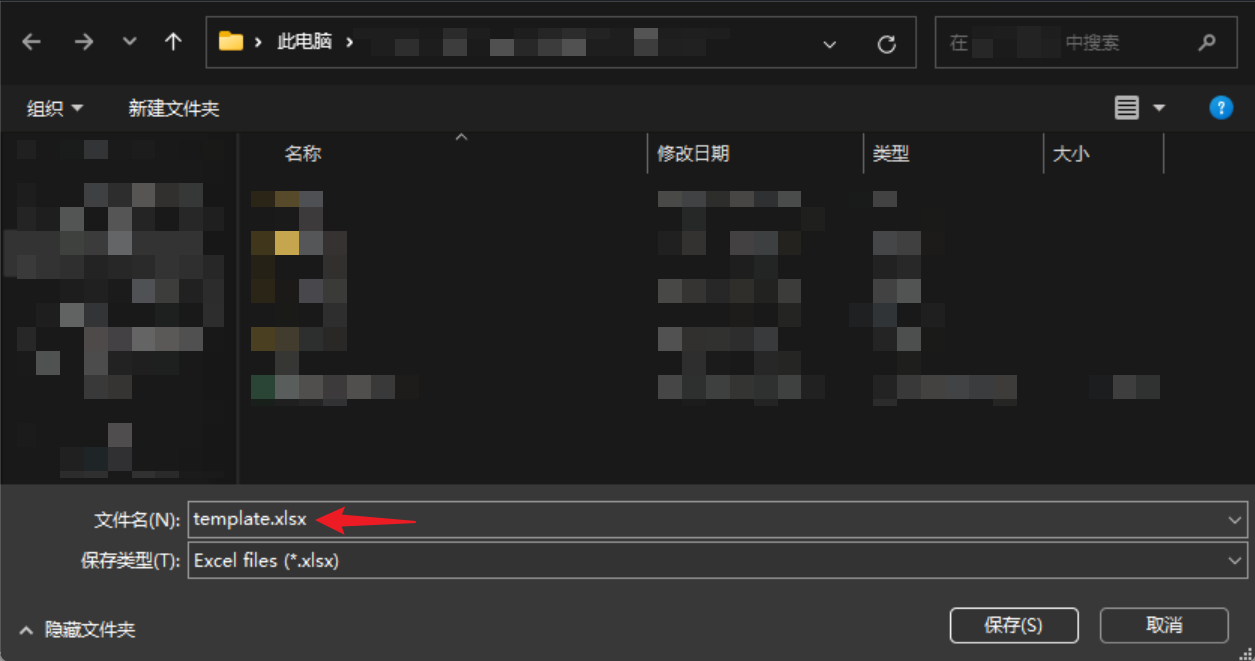
\includegraphics[width=0.7\linewidth]{fig/模板保存}
		\caption{选择模板文件的存储位置}
		\label{fig:选择模板文件的存储位置}
	\end{figure}
	\subsection{加分项目的信息填写}
	如图所示\ref{fig:加分项目的信息填写示例}，为加分项目的信息填写示例。
	\begin{figure}[H]
	\centering
	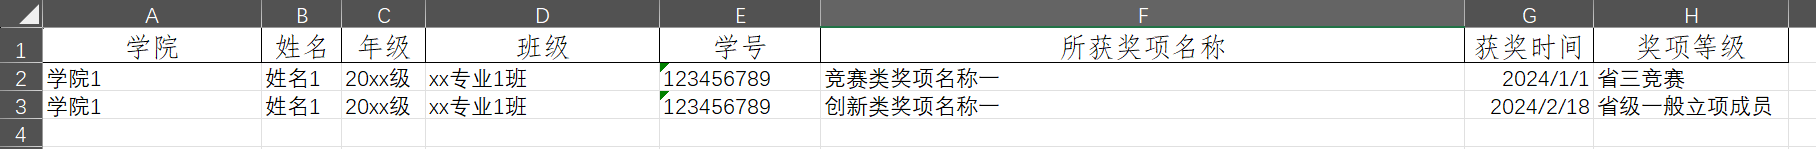
\includegraphics[width=0.7\linewidth]{fig/加分项信息填写示例}
	\caption{加分项目的信息填写示例}
	\label{fig:加分项目的信息填写示例}
\end{figure}	

	\textcolor{mygreen}{
	\subsection{自定义加分规则的数据收集}
	如图\ref{fig:版本V3.0评审界面新功能按钮展示}所示，版本V3.0新增加了“导入加分详情”的功能，支持从Excel文件导入自定义的项目类型、奖项级别和加分规则。}

	\textcolor{mygreen}{
	【导入加分详情】至少要求Excel文件包含三列内容：项目类型、奖项级别和加分规则。针对项目类型可能存在的加分上限，可在Excel第四列为每类项目设置统计分数上限，无则默认6分。如果存在同一项目类型的加分上限不同，则采用第一次该项目类型出现时对应的分数上限。
}

	\textcolor{mygreen}{
	加分详情Excel参考示例如图\ref{fig:版本3.0的加分详情参考示例}所示，要求列顺序和抬头文字如图一致，分别为“项目类型”，“奖项级别”，“加分”，“加分上限”。如若不提供加分上限，则默认每个项目类型的加分上限为6分。
}
	\begin{figure}[h]
		\centering
		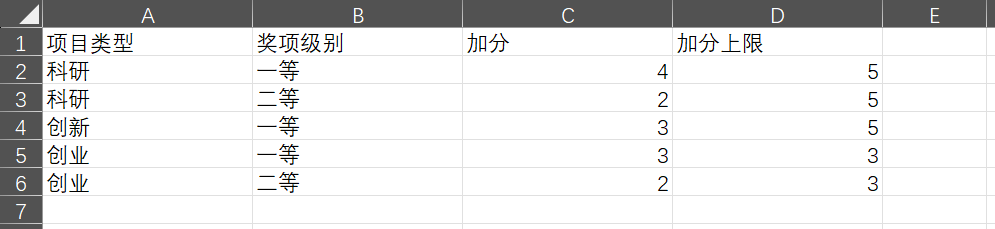
\includegraphics[width=0.7\linewidth]{fig/3.0加分详情参考示例}
		\caption{版本V3.0的加分详情参考示例}
		\label{fig:版本3.0的加分详情参考示例}
	\end{figure}
	
\section{注册}
	“注册”功能为导航栏第一个功能按钮，点击后如图\ref{fig:注册界面}所示。第一次使用本软件请注册账号，在未登录情况下，无法使用文件导入功能，即不能借助本软件开展评审工作，会有如图\ref{fig:未登录警告}所示弹窗提醒用户登录。
\begin{figure}[H]
	\centering
	\begin{minipage}{0.45\linewidth}  % 调整宽度以适应两张图并排
		\centering
		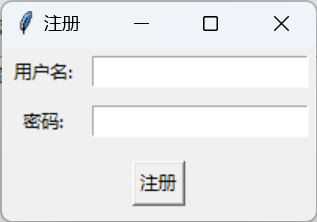
\includegraphics[width=\linewidth]{fig/注册界面}
		\caption{用户注册界面}
		\label{fig:注册界面}
	\end{minipage}%
	\hspace{0.05\linewidth}  % 调整两个图像之间的水平间距
	\begin{minipage}{0.45\linewidth}
		\centering
		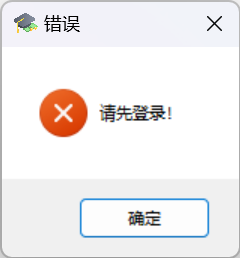
\includegraphics[width=0.75\linewidth]{fig/未登录无法导入文件警告}
		\caption{未登录无法导入文件警告提示}
		\label{fig:未登录警告}
	\end{minipage}
\end{figure}


注册账户时，需要输入用户名和密码，用户名可以是文字、数字、字母、符号诸如此类的文本内容，密码同样支持。如果在注册时缺少两者之一，会弹窗警告如图\ref{fig:注册错误警告界面}所示。当注册用户名为已注册用户时，会提示“该账户已存在”，如图\ref{fig:重复注册警告}所示。\textbf{请第一次注册时，妥善记录和保存用户名和密码。}
\begin{figure}[H]
	\centering
	\begin{minipage}{0.45\linewidth}
		\centering
		
\includegraphics[width=\linewidth]{fig/注册错误警告界面}
		\caption{注册错误警告界面}
		\label{fig:注册错误警告界面}
	\end{minipage}
	\hspace{0.05\linewidth}  % 这行可以调整图像间的水平间距
	\begin{minipage}{0.45\linewidth}
		\centering
		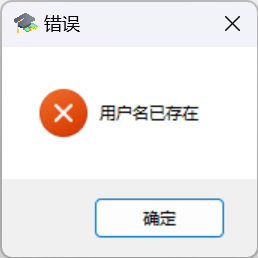
\includegraphics[width=0.85\linewidth]{fig/重复注册警告}
		\caption{重复注册警告}
		\label{fig:重复注册警告}
	\end{minipage}
\end{figure}

	\section{登录}
	“登录”功能为导航栏第二个功能按钮，点击后如图\ref{fig:登录界面}所示。在未登录情况下，无法使用文件导入功能，即不能借助本软件开展评审工作，会有如图\ref{fig:未登录警告1}所示弹窗提醒用户登录。
	
	
	\begin{figure}[H]
		\centering
		\begin{minipage}{0.45\linewidth}  % 调整宽度以适应两张图并排
			\centering
			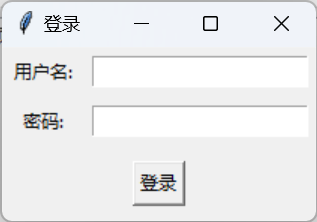
\includegraphics[width=\linewidth]{fig/登录界面}
			\caption{用户登录界面}
			\label{fig:登录界面}
		\end{minipage}%
		\hspace{0.05\linewidth}  % 调整两个图像之间的水平间距
		\begin{minipage}{0.45\linewidth}
			\centering
			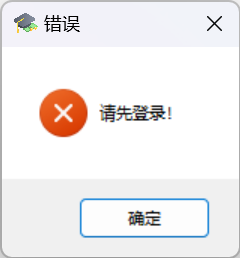
\includegraphics[width=0.7\linewidth]{fig/未登录无法导入文件警告}
			\caption{未登录无法导入文件警告提示}
			\label{fig:未登录警告1}
		\end{minipage}
	\end{figure}
	
	
	
	登录账户时，需要输入用户名和密码。如果在登录时缺少两者之一，会弹窗警告如图\ref{fig:登录错误警告界面}所示。如果输入的用户名不存在，会如图\ref{fig:用户名不存在提醒}所示弹窗提示用户名不存在，请用户进行注册或检查是否存在输入错误的情况。
	\begin{figure}[H]
	\centering
	\begin{minipage}{0.45\linewidth}  % 调整宽度以适应两张图并排
		\centering
		
\includegraphics[width=\linewidth]{fig/登录错误警告界面}
		\caption{登录错误警告界面}
		\label{fig:登录错误警告界面}
	\end{minipage}%
	\hspace{0.05\linewidth}  % 调整两个图像之间的水平间距
	\begin{minipage}{0.45\linewidth}
		\centering
	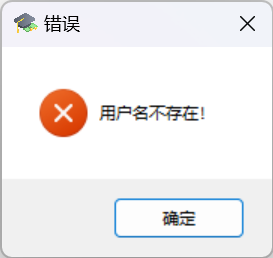
\includegraphics[width=0.85\linewidth]{fig/用户不存在提醒}
	\caption{用户名不存在提醒}
	\label{fig:用户名不存在提醒}
	\end{minipage}
\end{figure}		
	

	如果出现密码输入错误的情况，会如图\ref{fig:密码错误提醒}所示弹窗提示密码输入错误。本软件为用户提供同用户名三次密码输入的机会，若三次输入密码都错误，会将锁定当前用户名，如图\ref{fig:账户锁定错误界面}所示，需在输入管理员密码（解锁密码）后才能解锁用户。\textbf{本软件管理员密码（解锁密码）暂定为“deblocking”，账户解锁成功界面如图\ref{fig:账号解锁deblocking界面}所示}。
	
	\begin{figure}[H]
	\centering
	\begin{minipage}{0.3\linewidth}  % 调整宽度以适应两张图并排
		\centering
		
\includegraphics[width=\linewidth]{fig/密码错误提醒}
		\caption{密码输入错误界面}
		\label{fig:密码错误提醒}
	\end{minipage}%
	\hspace{0.03\linewidth}  % 调整两个图像之间的水平间距
	\begin{minipage}{0.3\linewidth}
		\centering
		
\includegraphics[width=\linewidth]{fig/账户锁定界面}
		\caption{账户锁定错误界面}
		\label{fig:账户锁定错误界面}
	\end{minipage}
		\hspace{0.03\linewidth}
		\begin{minipage}{0.3\linewidth}
		\centering
		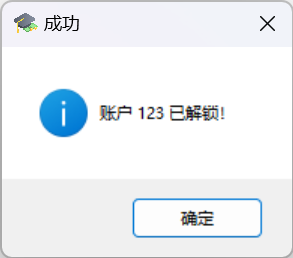
\includegraphics[width=0.95\linewidth]{fig/账号解锁deblocking界面}
		\caption{账号解锁界面}
		\label{fig:账号解锁deblocking界面}
	\end{minipage}
\end{figure}	

	\section{关于}
	“关于”功能为导航栏第三个功能按钮，点击后如图\ref{fig:关于界面}所示，将展示本软件的版权所有信息，后续会根据实际需求继续增设内容，以便更好地宣传本软件。
	
\textbf{\textcolor{mygreen}{考虑到版本更新问题，即版本号会进行更新，但如若版权所有人未出现修改，使用说明书的关于界面不进行更新，而实际代码和程序会进行更新。}}
		\begin{figure}[H]
			\centering
			
\includegraphics[width=0.5\linewidth]{fig/关于界面}
			\caption{关于界面}
			\label{fig:关于界面}
		\end{figure}
		
	\section{帮助}
	“帮助”功能为导航栏第四个功能按钮，点击后如图\ref{fig:帮助界面}所示，将展示简要的使用说明，后续会根据软件反馈继续增设内容，以提供用户更好的服务。
		\begin{figure}[H]
			\centering
			
\includegraphics[width=0.5\linewidth]{fig/帮助界面}
			\caption{帮助界面}
			\label{fig:帮助界面}
		\end{figure}

	\section{模板}
	“模板”功能为导航栏第五个功能按钮，点击后如图\ref{fig:模板保存}所示，选择模板文件保存的位置即可。默认模板文件保存格式为“template.xlsx”，默认模板文件保存位置为软件所在目录。
	\begin{figure}[H]
	\centering
	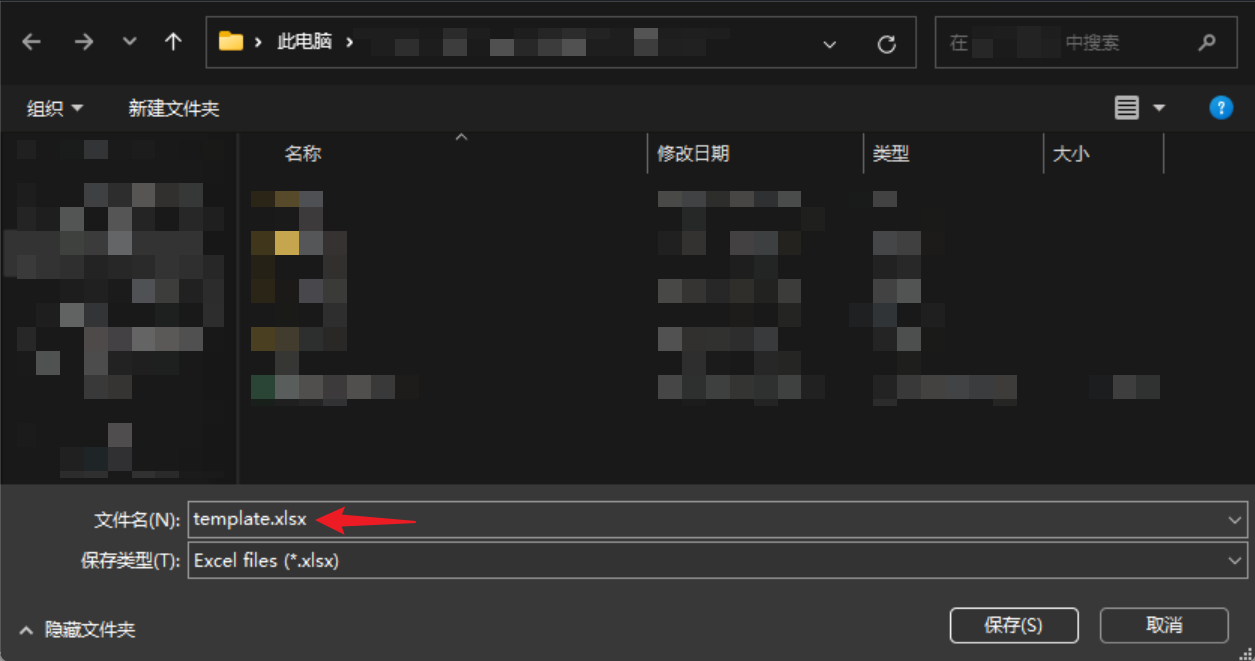
\includegraphics[width=0.5\linewidth]{fig/模板保存}
	\caption{模板保存界面}
	\label{fig:模板保存}
\end{figure}	
	
	\section{浅色/深色模式}
	“浅色模式”和“深色模式”功能为导航栏第六和第七个功能按钮，点击后分别如图\ref{fig:浅色界面}和图\ref{fig:深色界面}所示，软件启动默认为浅色模式，用户可视个人使用习惯切换浅色/深色模式。


	\begin{figure}[H]
	\centering
	\begin{minipage}{0.45\linewidth}  % 调整宽度以适应两张图并排
		\centering
		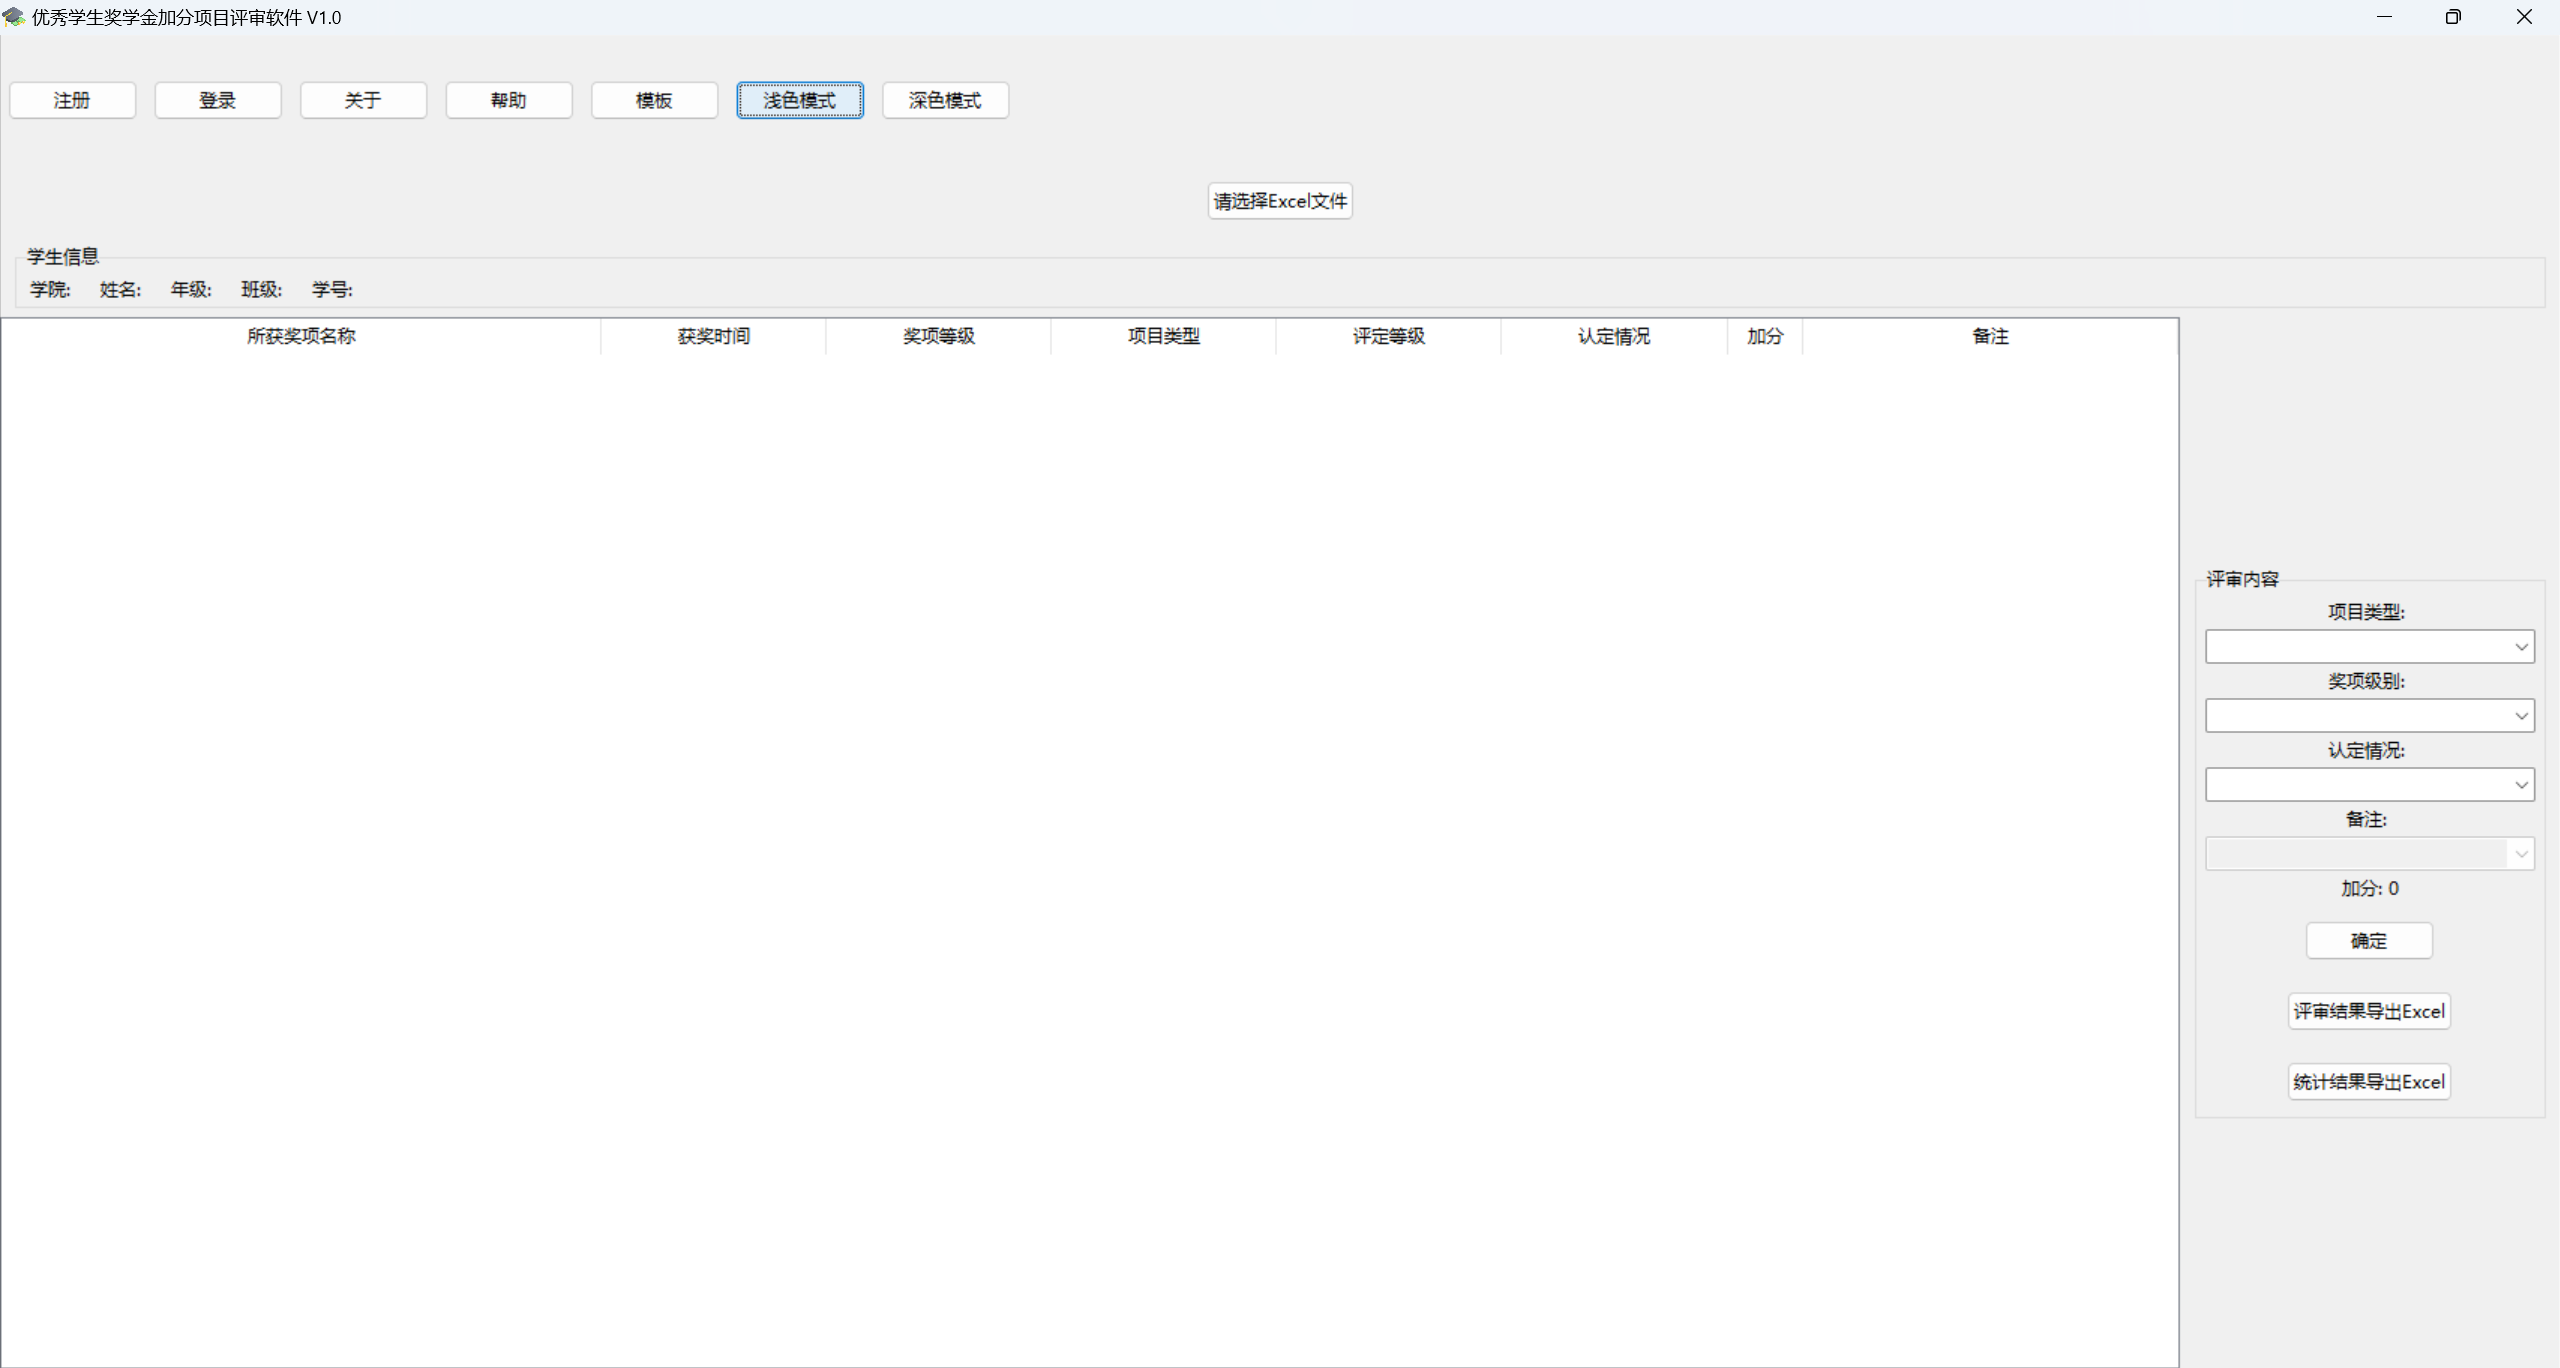
\includegraphics[width=\linewidth]{fig/浅色界面}
		\caption{浅色模式界面}
		\label{fig:浅色界面}
	\end{minipage}%
	\hspace{0.05\linewidth}  % 调整两个图像之间的水平间距
	\begin{minipage}{0.45\linewidth}
		\centering
		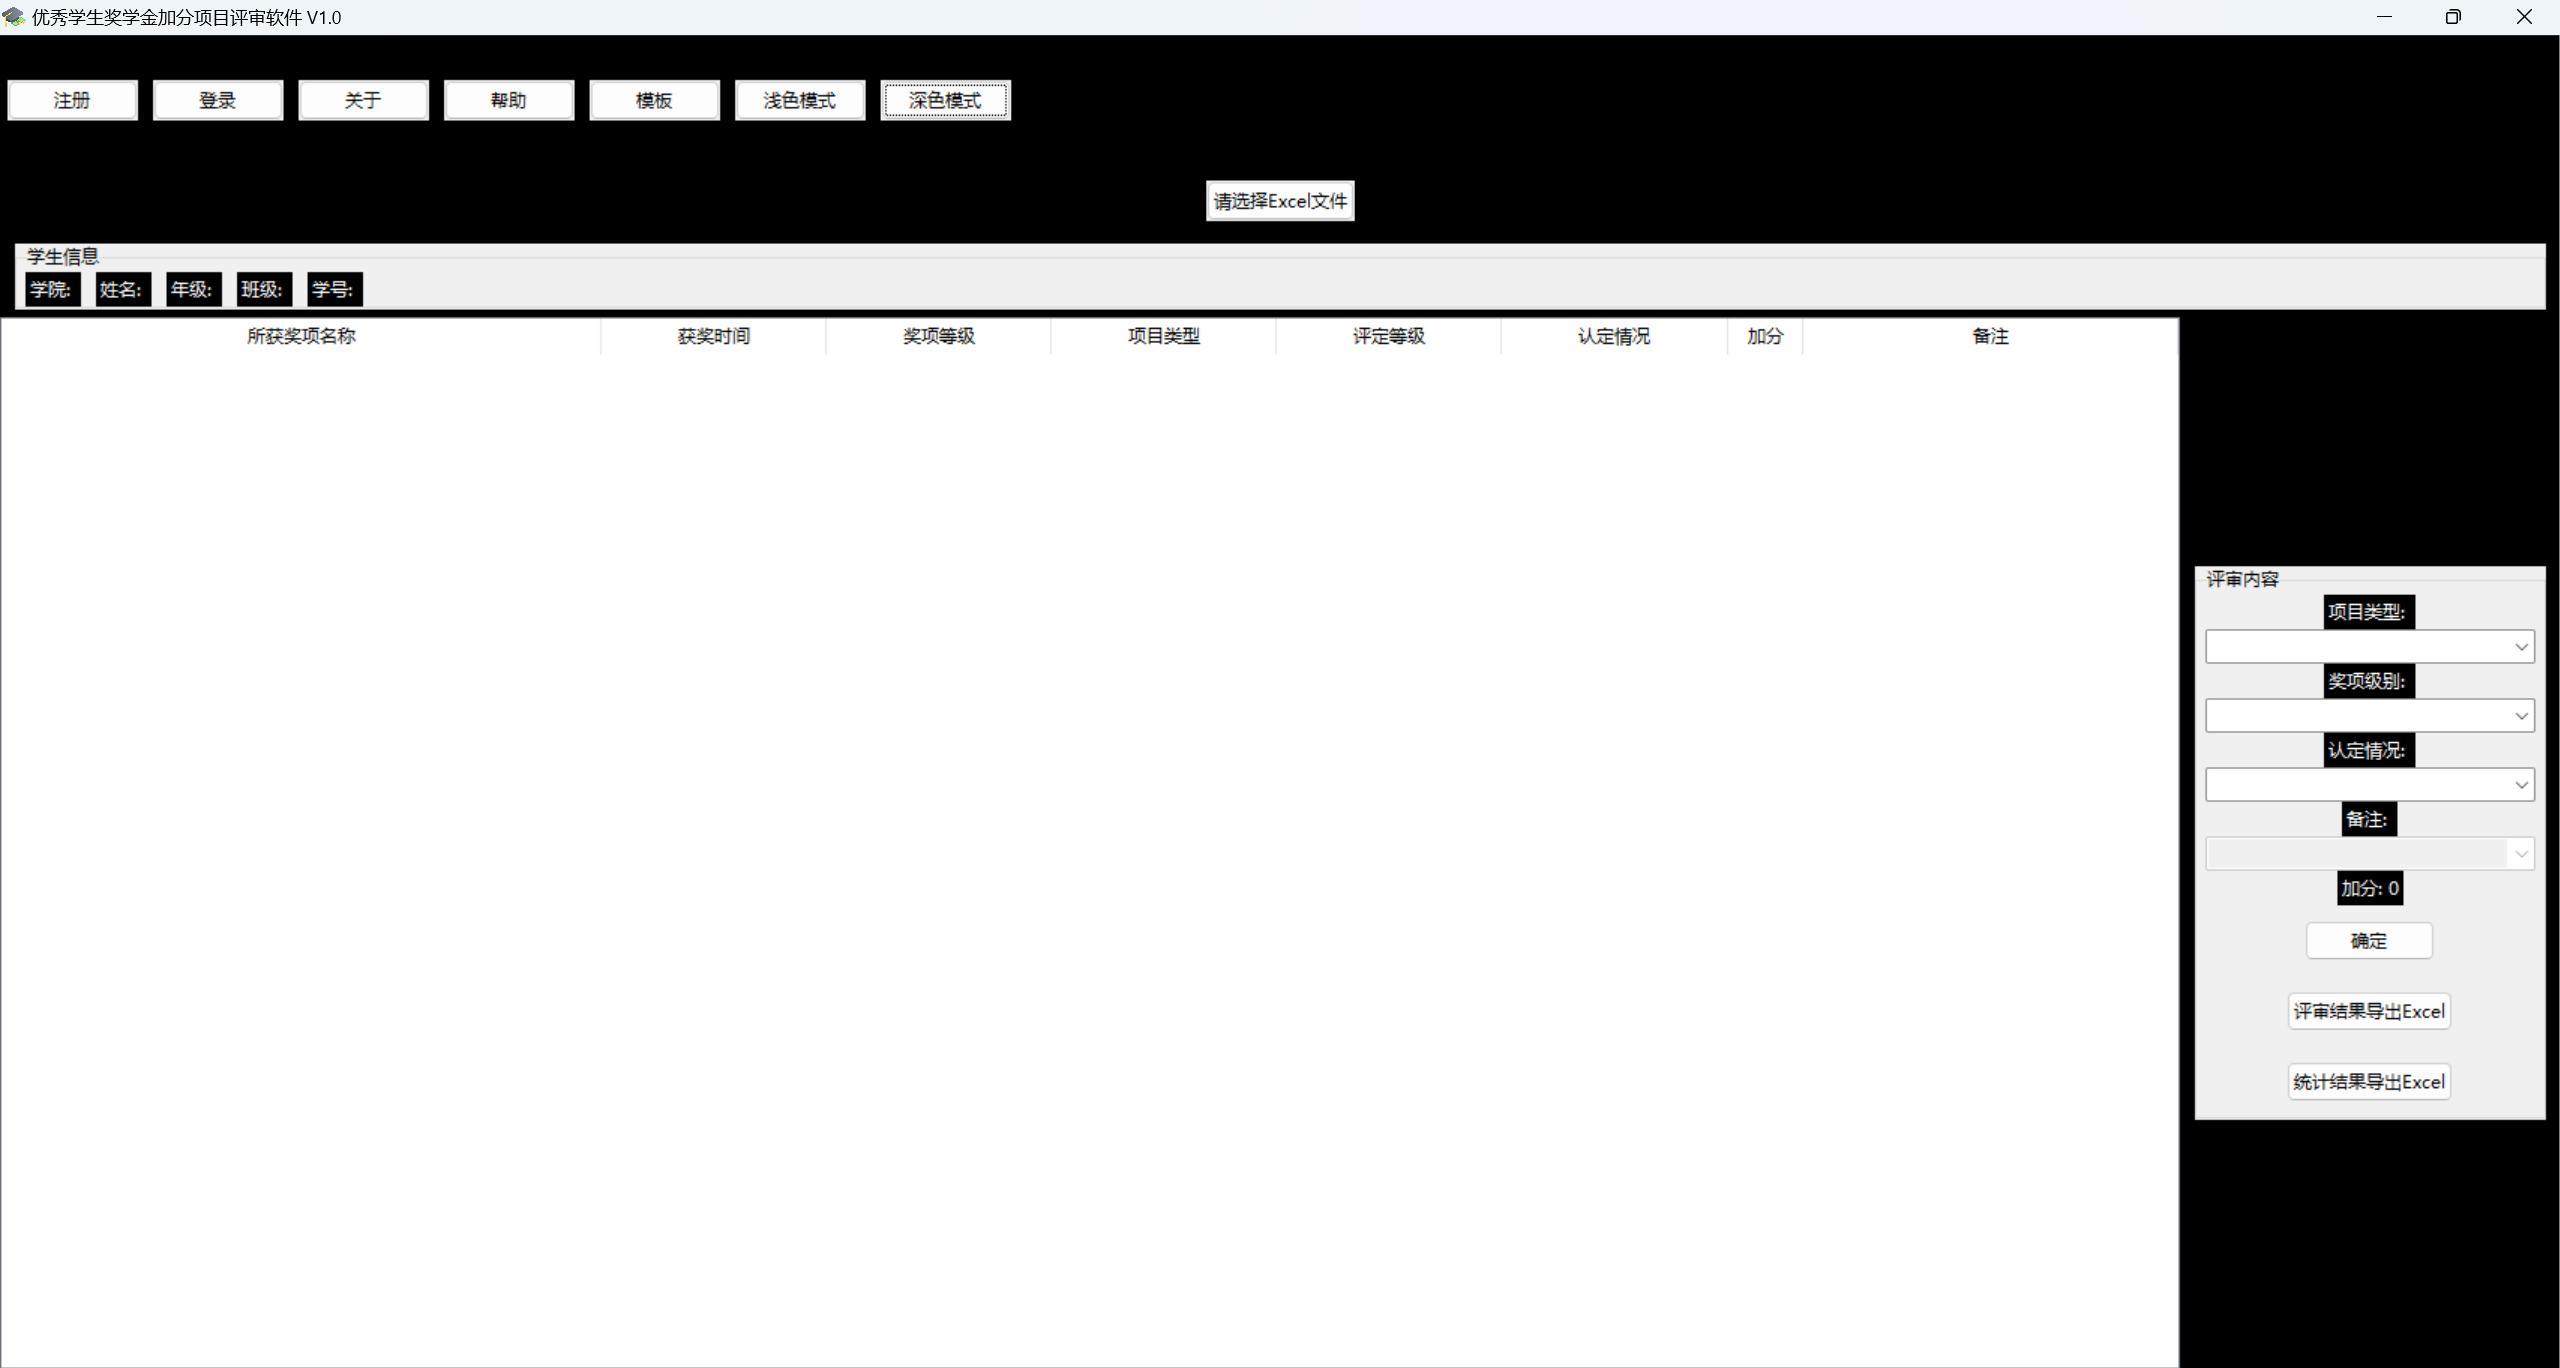
\includegraphics[width=\linewidth]{fig/深色模式}
		\caption{深色模式界面}
		\label{fig:深色界面}
	\end{minipage}
\end{figure}

	\section{文件导入}
	如图\ref{fig:文件导入按钮}所示为文件导入按钮，点击后选取由申请加分项目人员递交的已填写的Excel文件即可。正确导入后的界面会如图\ref{fig:文件已加载}所示弹窗提示“文件已加载”，评审界面也会更新至如图\ref{fig:导入文件后的评审界面}所示，届时可看到递交人员的基本信息和加分项目信息。
	\begin{figure}[h]
		\centering
		
\includegraphics[width=0.7\linewidth]{fig/文件导入按钮}
		\caption{文件导入按钮}
		\label{fig:文件导入按钮}
	\end{figure}
	
		\begin{figure}[H]
		\centering
		\begin{minipage}{0.45\linewidth}  % 调整宽度以适应两张图并排
			\centering
			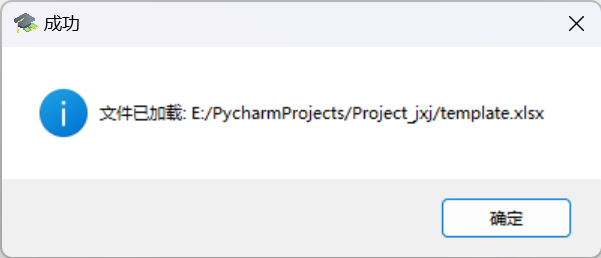
\includegraphics[width=\linewidth]{fig/文件已加载}
			\caption{文件已加载提醒}
			\label{fig:文件已加载}
		\end{minipage}%
		\hspace{0.05\linewidth}  % 调整两个图像之间的水平间距
		\begin{minipage}{0.45\linewidth}
			\centering
			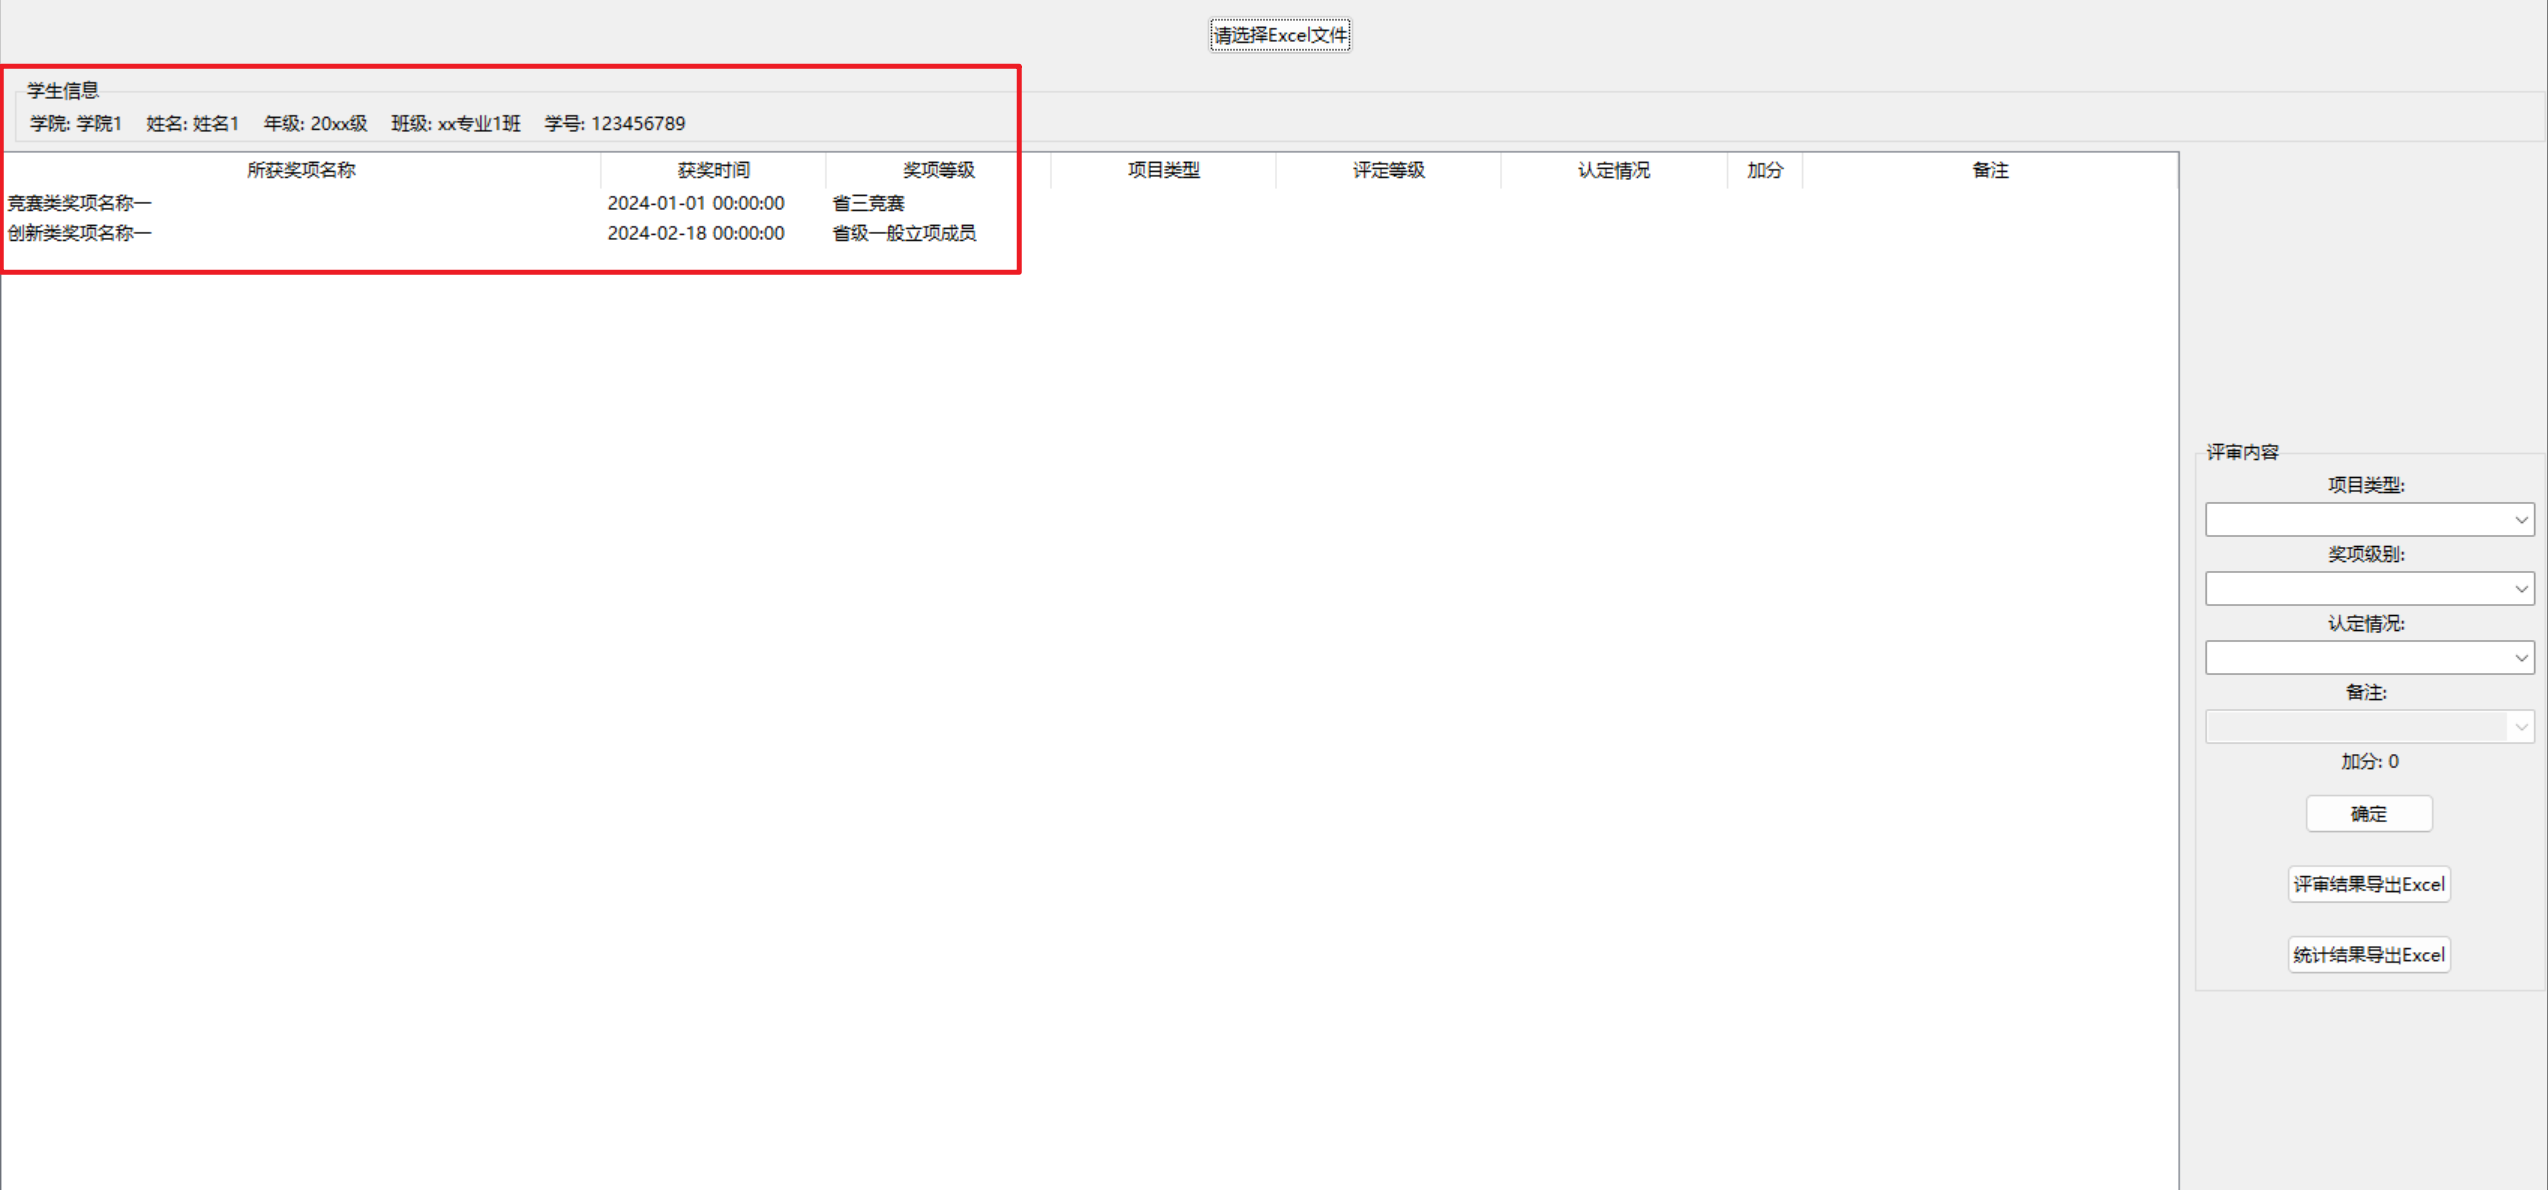
\includegraphics[width=\linewidth]{fig/导入文件后的评审界面}
			\caption{导入文件后的评审界面}
			\label{fig:导入文件后的评审界面}
		\end{minipage}
	\end{figure}
	
	
		\textcolor{mygreen}{
		版本V3.0更新的内容有：【批量导入Excel文件】支持一次导入多个学生，支持大规模评审。导入过程支持文件格式验证（自动验证每个文件是否包含必要的列（学院、姓名、年级、班级、学号等）），重复检查（防止导入相同学生的数据）和错误处理（详细显示导入成功和失败的文件信息）。完成导入后可通过“学生选择下拉菜单”便捷切换不同学生的评审数据，如图\ref{fig:版本V3.0学生选择下拉菜单展示}所示。
	}
	

	
	\textcolor{mygreen}{
		【补充导入Excel文件】支持在已有数据基础上追加导入新的学生Excel文件，无需重新选择所有文件。为了方便评审工作的开展，在单个文件导入评审的情况下，选择补充导入会自动转化为批量处理状态，届时同样可通过“学生选择下拉菜单”便捷切换不同学生的评审数据。
	}
	
	
	
	\textcolor{myred}{
    \section{支撑材料预览}
    如图\ref{fig:图片奖项展示}和图\ref{fig:pdf奖项示例}所示，为支撑材料预览展示。图片类型的文件可以直接显示，pdf类型的文件可点击打开按钮进行显示。此举可方便评审人员无需重复进行界面切换，减轻工作量。
}

    \textcolor{myred}{
    \textbf{需要注意，支撑材料的文件名需要与Excel材料表中填写的奖项名称保持一致，否则将无法正确读取。}
    \begin{figure}[h]
    	\centering
    	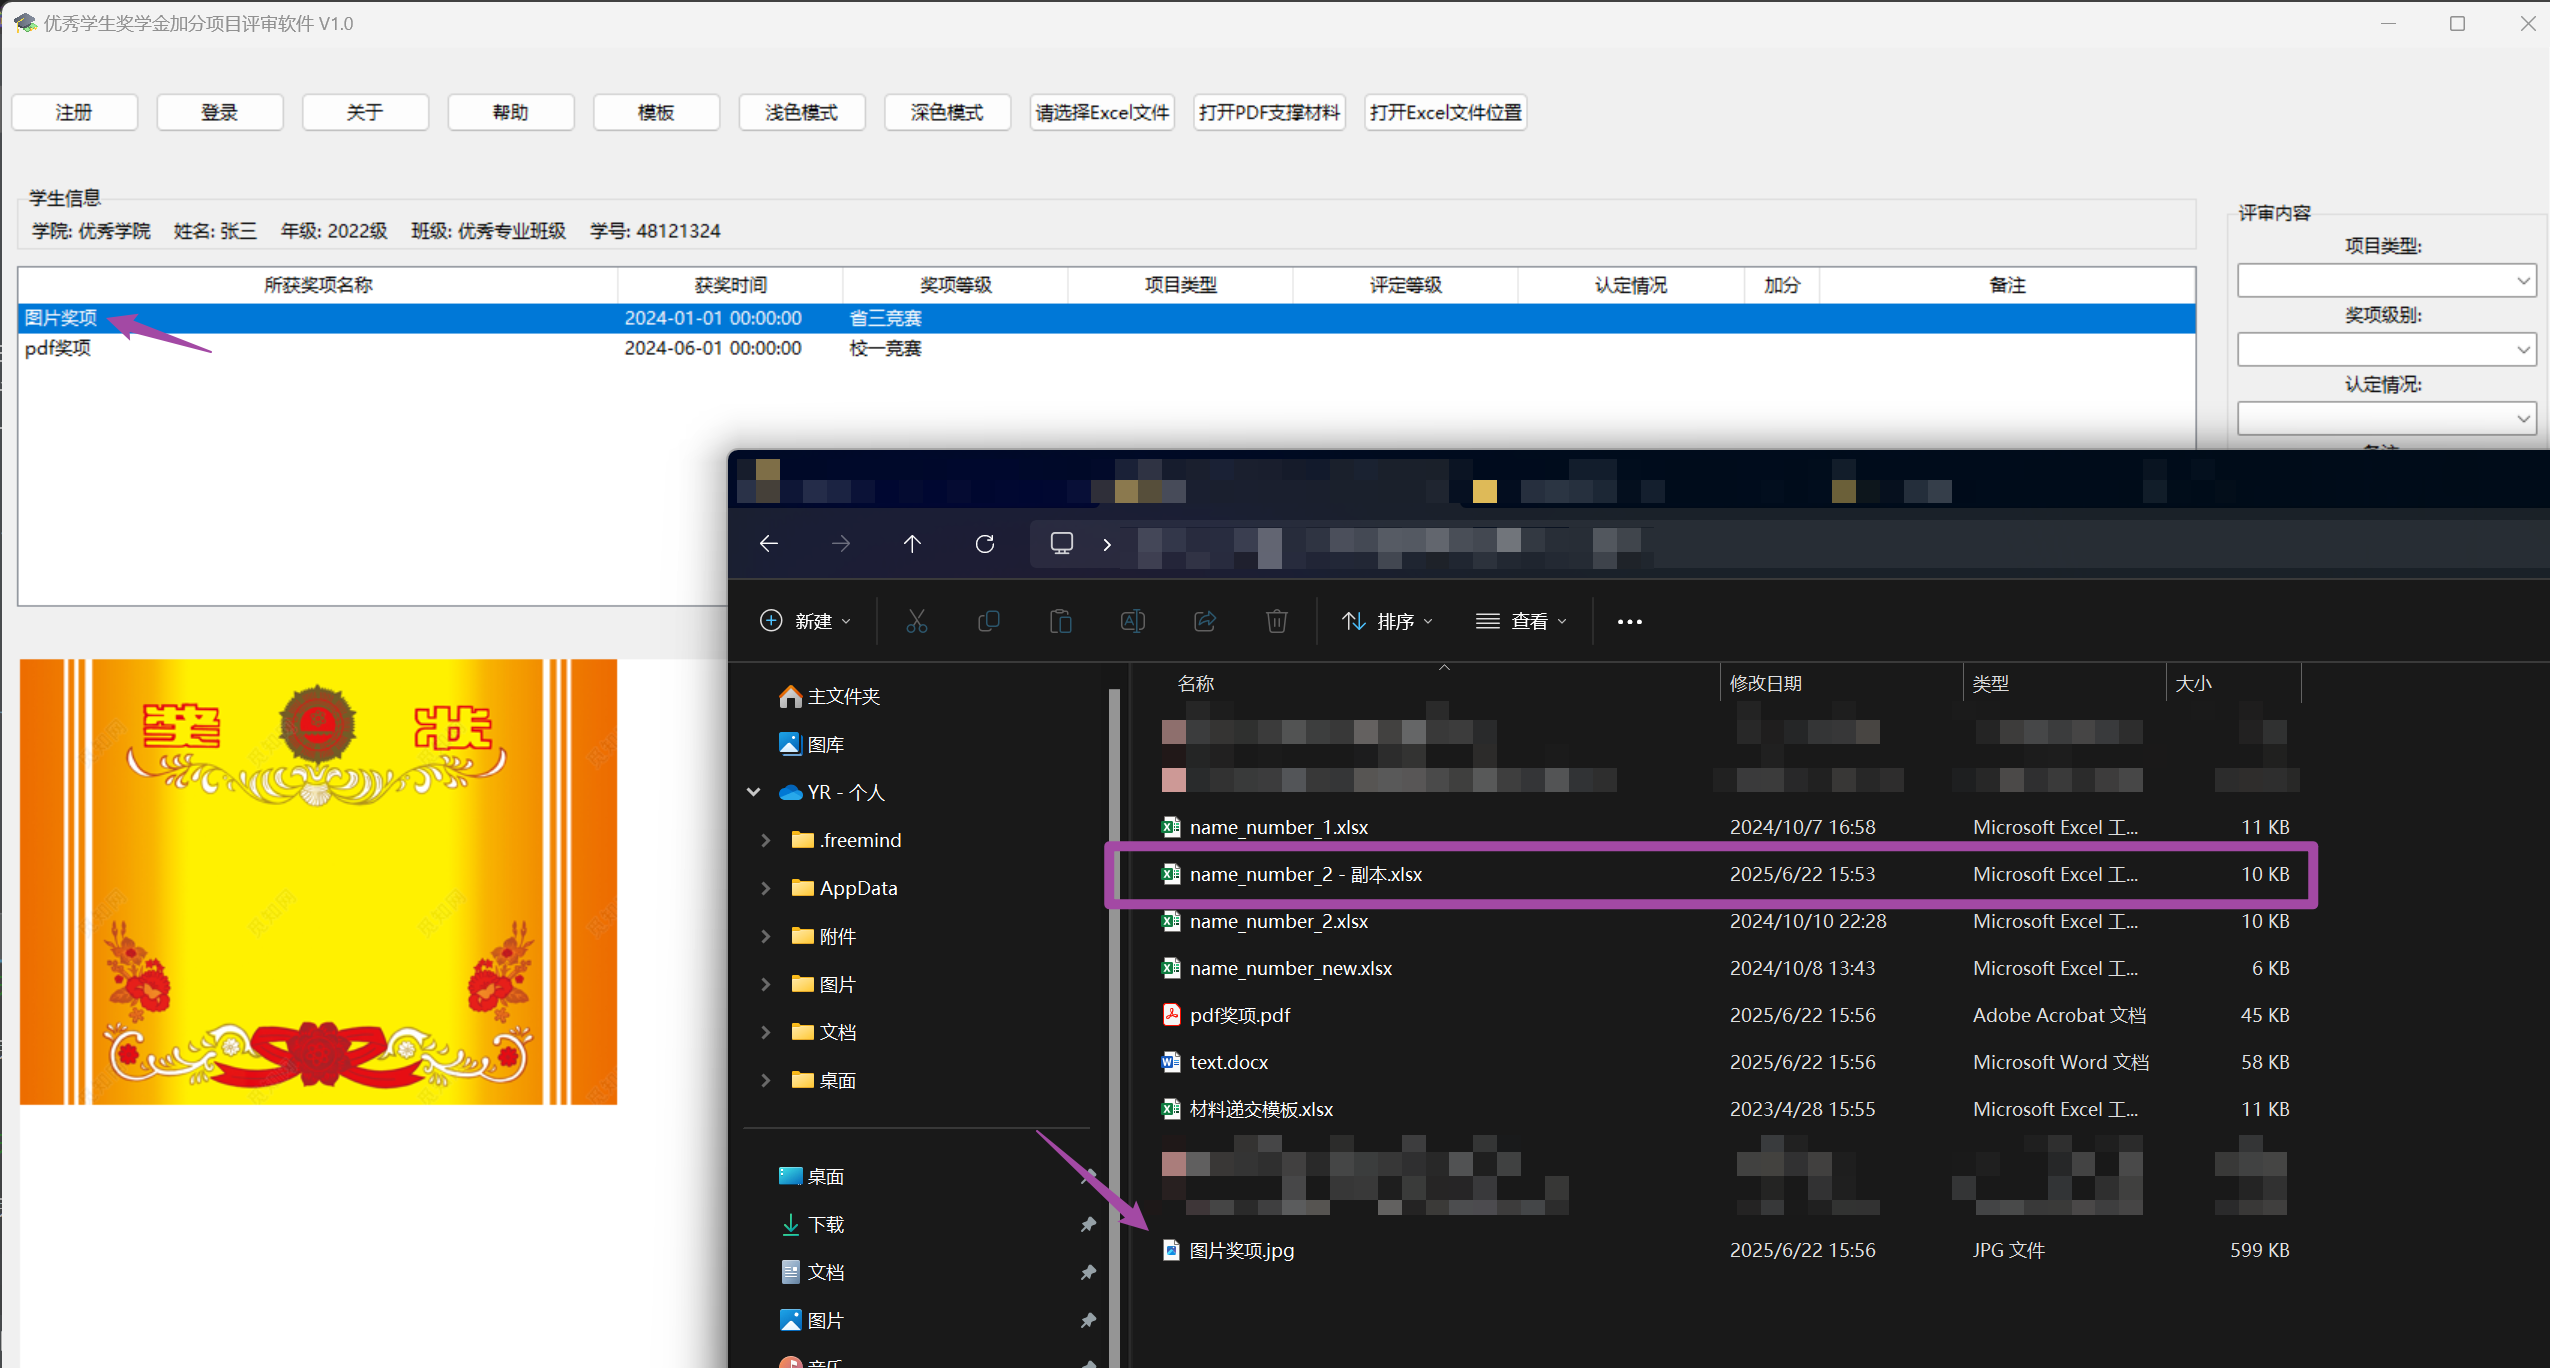
\includegraphics[width=0.7\linewidth]{fig/图片奖项展示}
    	\caption{图片奖项展示}
    	\label{fig:图片奖项展示}
    \end{figure}    
    \begin{figure}[h]
    	\centering
    	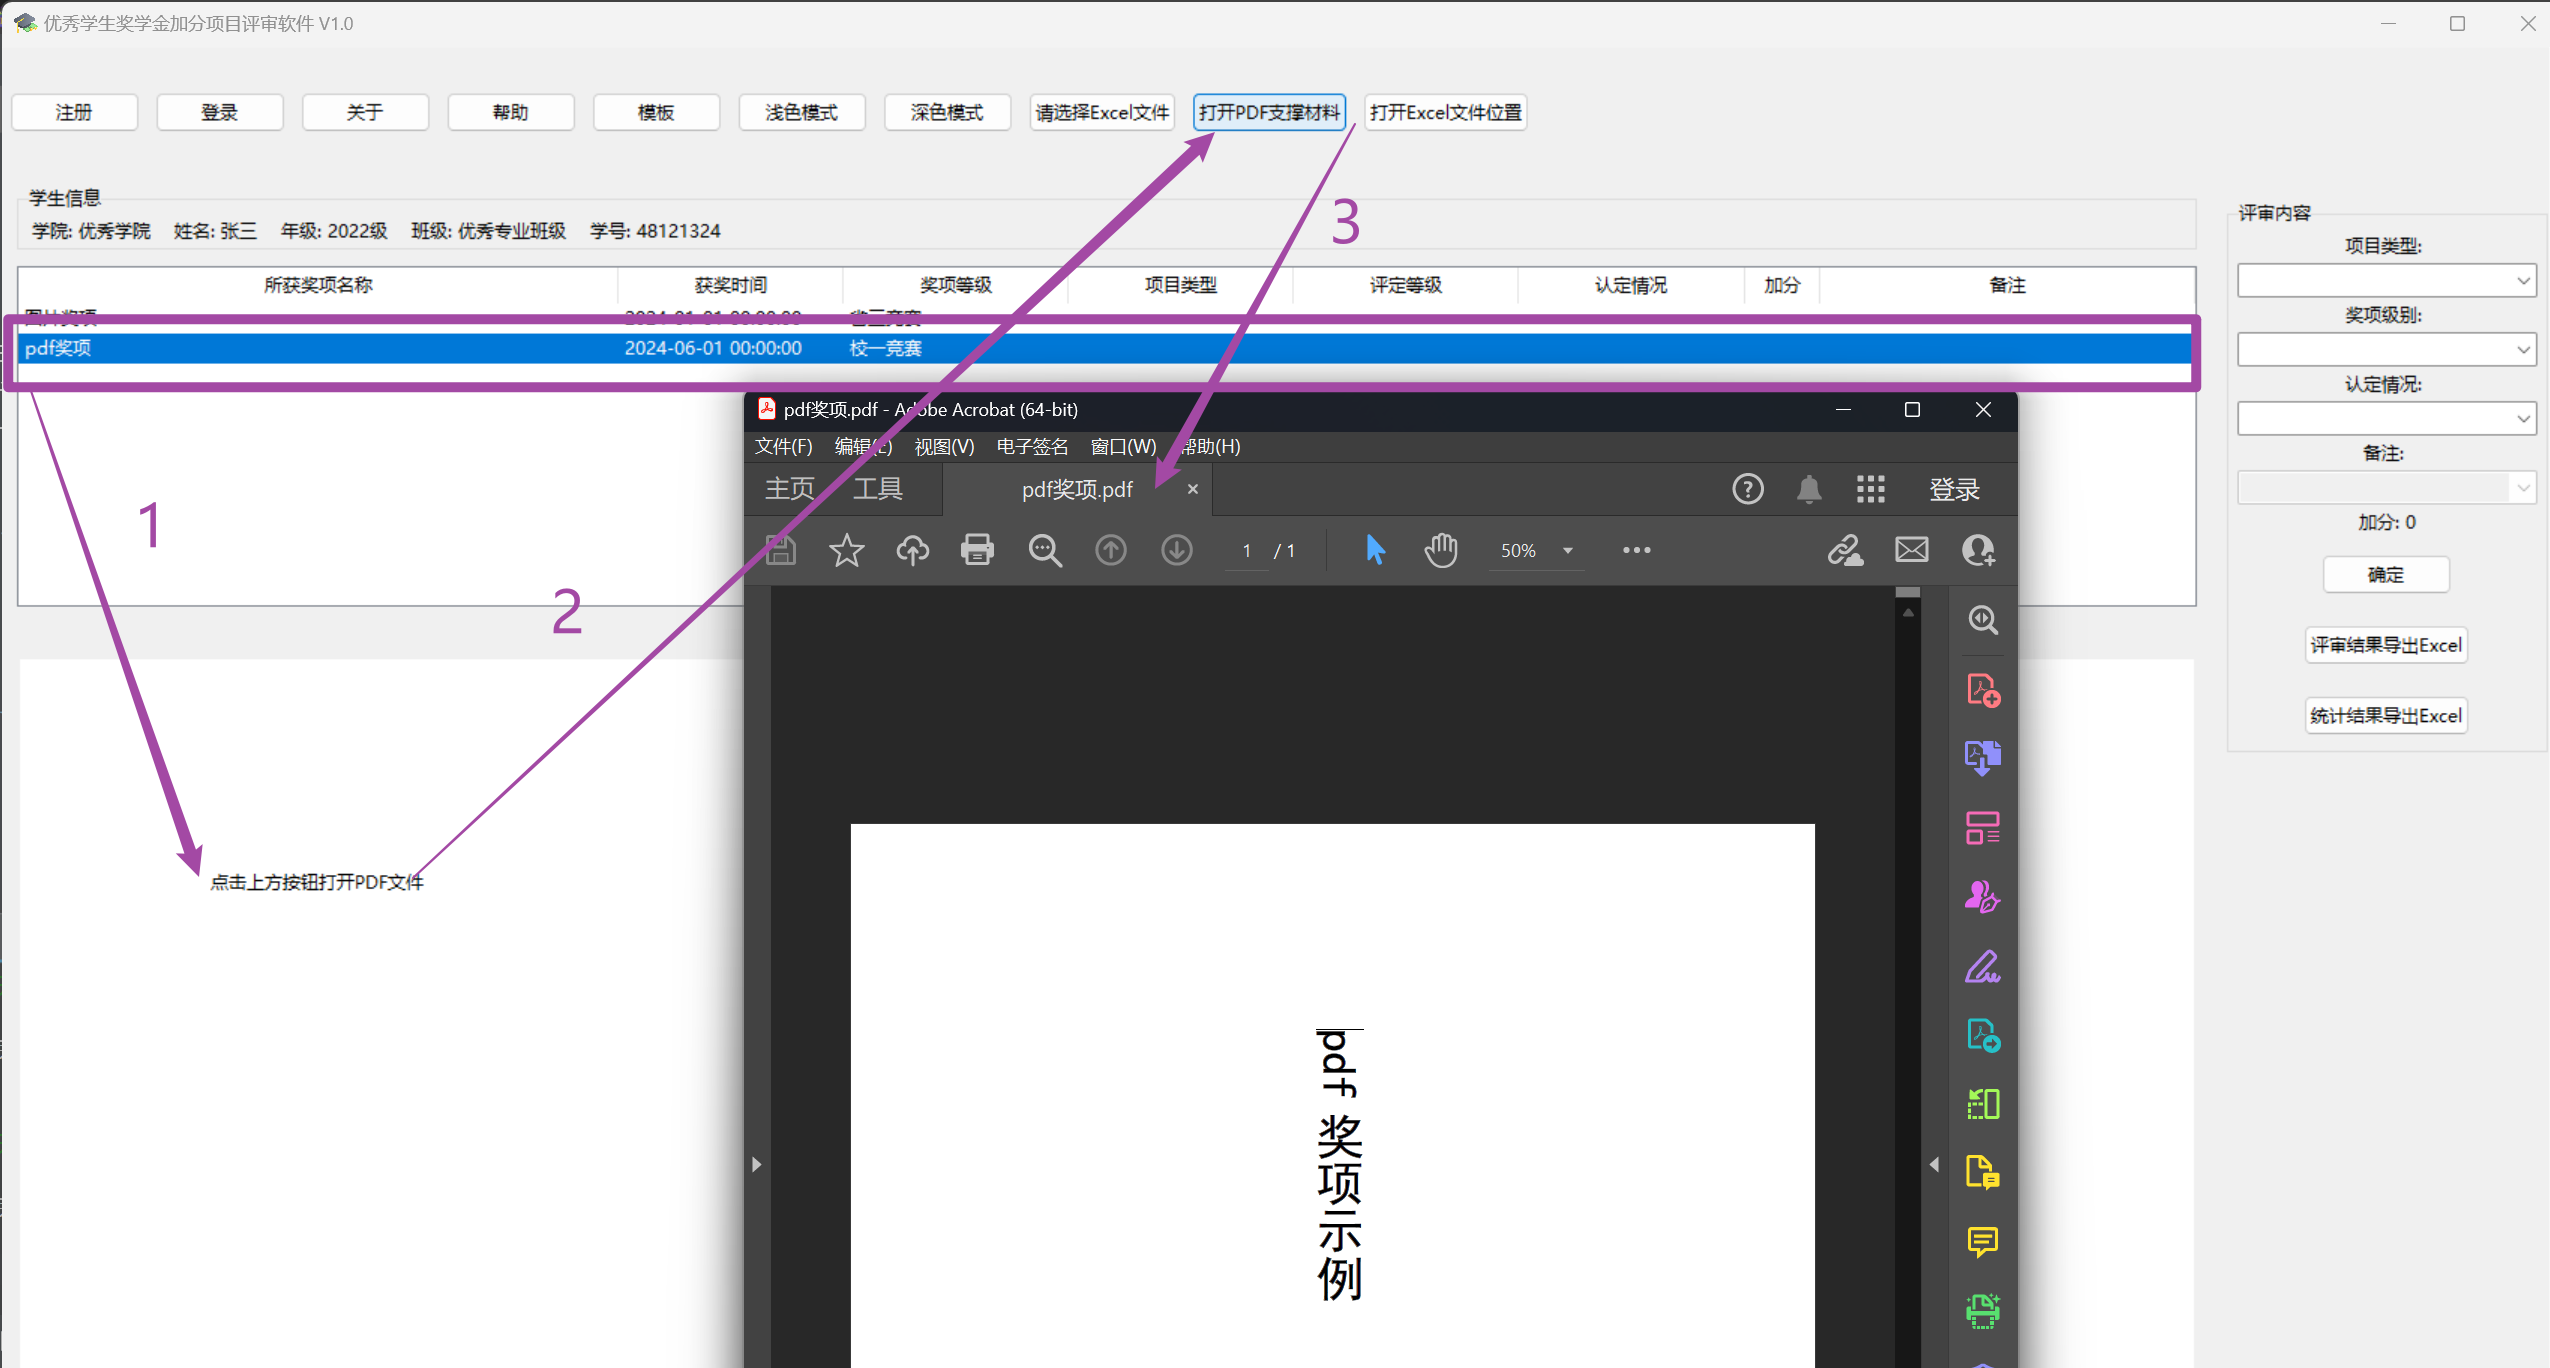
\includegraphics[width=0.7\linewidth]{fig/pdf奖项示例}
    	\caption{pdf奖项示例}
    	\label{fig:pdf奖项示例}
    \end{figure}
    } 

	\section{评审}
	\subsection{评审细则及注意事项}
	在开展评审工作前，了解评审的要求和不同加分项目的加分情况尤为重要，在本软件中，默认的加分项目类型为“竞赛类加分”，“科研创新类加分”，“外语类加分”三类，其下根据奖项级别的不同，“竞赛类加分”有15种不同的分值，“科研创新类加分”有27种不同的分值，“外语类加分”有12种不同的分值，详情如表\ref{分值表}所示。


对于加分项目的评定等级的认定需要根据申请人递交的支撑材料的文件内容、盖章单位进行确认，并非依据申请人填写的奖项等级进行认定。

\textcolor{mygreen}{
对于希望采用新的加分项目分值表，可以通过【导入加分详请】实现在默认规则和自定义规则之间切换，具体要求可参见前文中“自定义加分规则的数据收集”部分的内容。同时亦可通过【重置为默认】一键恢复到系统默认的加分规则。
}

	\subsection{评审操作}
	在完成文件导入后评审界面已更新至如图\ref{fig:导入文件后的评审界面}所示，此时评审人员可在评审内容区域开展评审工作：判断该加分项目的所属项目类型，奖项级别，认定情况，备注等信息。
	
	评审人员要先选择某一加分项目后再在评审内容内进行选择该加分项目的所属项目类型，奖项级别，认定情况，备注等信息，否则将无法该加分项目的所属项目类型，奖项级别，认定情况，备注等信息纳入评审界面。
	
	“奖项级别”下拉菜单会根据“项目类型”进行更新菜单选择。默认情况下“备注”下拉菜单为灰色，即不可选择状态，唯有“认定情况”为“不予认定”时，才会解锁。
	
	“认定情况”下拉菜单中，有“认定”和“不予认定”两种选项，当加分项目符合以下任一情况，即可不予认定该加分项目，届时需要在“备注”下拉菜单中选择对应的不予认定情况（此处需注意，即使不选择备注也可以进行确定），否则将影响后续评审结果和统计结果的导出。
	\begin{enumerate} 
	\item   时间不符，不予认定；
	\item 	名次不符，不予认定；	
	\item	该材料不符合本次奖项加分材料认定范围，不予认定；
	\item	支撑材料不足，补交（项目建设任务书、刊物等等）后可认定；
	\item	同一赛事奖项已认定最高分，不予重复加分；
	\item	线上比赛不符合认定要求，不予认定
	\item	其他（需补充文本内容）。
	\end{enumerate}

	\section{评审结果确定}
	如图\ref{fig:加分项目评审确定}所示，对示例文件中的第一个加分项目进行评审，点击“确认”后，即可将评审结果添加到该项目。
	\begin{figure}[H]
		\centering
		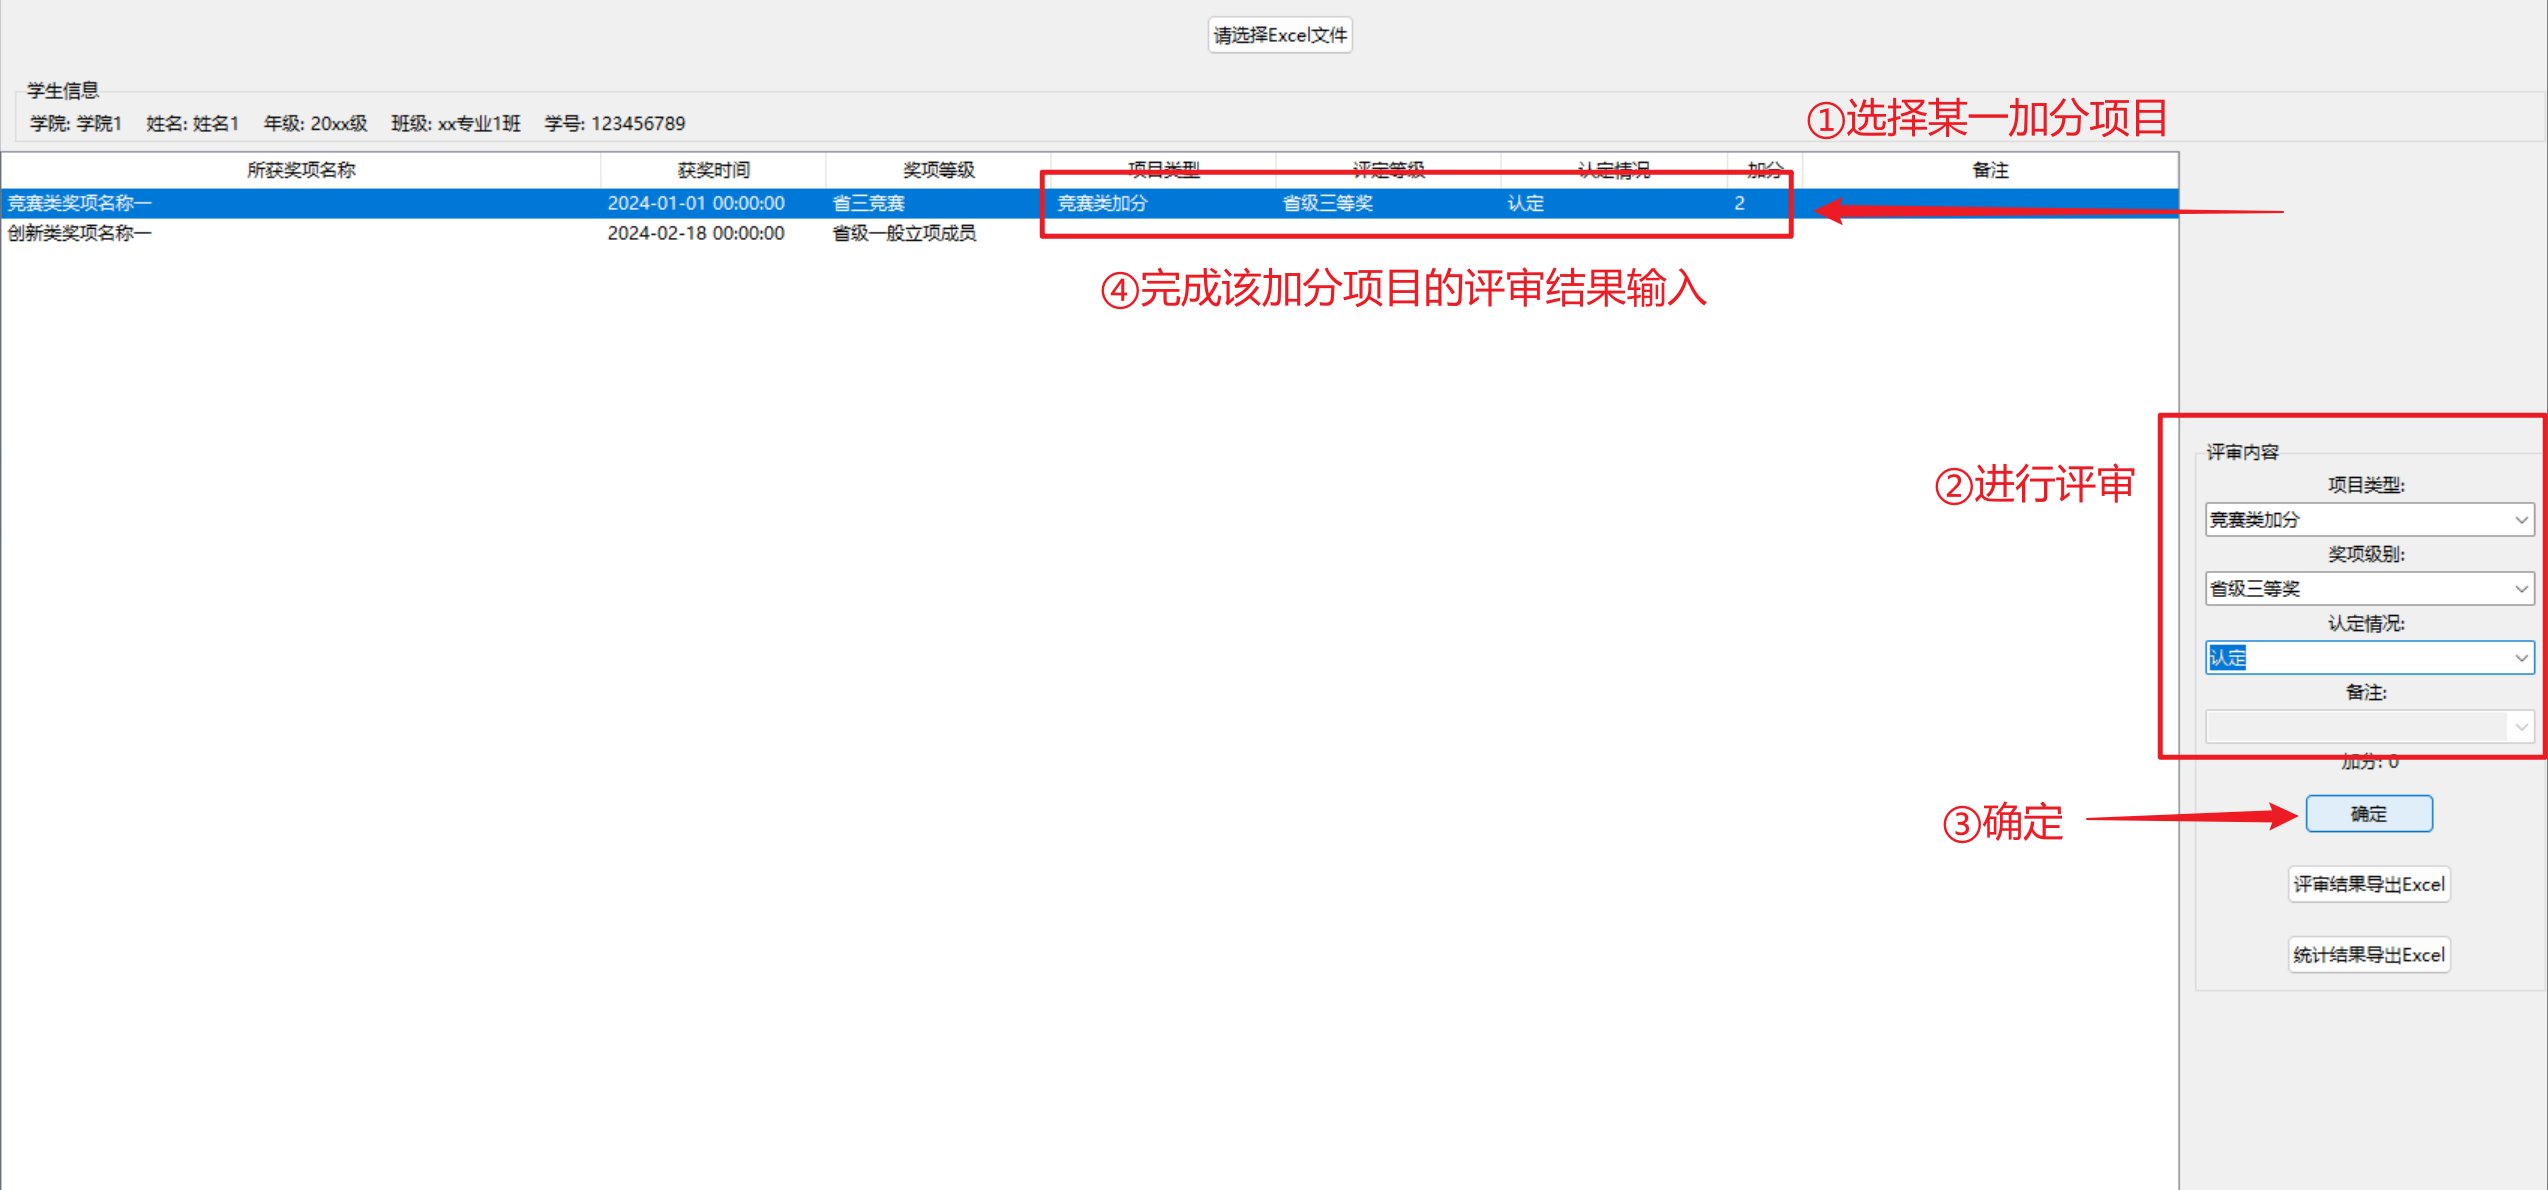
\includegraphics[width=0.5\textwidth]{fig/加分项目评审步骤}
		\caption{加分项目评审“确定”后的界面}
		\label{fig:加分项目评审确定}
	\end{figure}
	
	当“确定”完成某一加分项目后，本软件会自动跳转到下一加分项目，如果已是最后一项，则会重新检查所有的加分项目是否已全部完成评审，如存在还没评审的项目，亦会跳转到此未完成的项目，避免疏漏。
	
	当“确定”完成某一加分项目后，需要更改评审内容，需重新选中该项目，重复评审步骤，再次“确定”即可覆写上一次的评审结果。
	
	确认加分项目需注意要完成“项目类型”，“奖项级别”，“认定情况”，“备注”四个评审工作，仅对“认定情况”进行评定而不进行“项目类型”、“奖项级别”的评定会如图\ref{fig:“项目类型”和“奖项级别”不能为空提醒}所示弹窗提醒用户此两项不能为空。
	\begin{figure}[H]
		\centering
		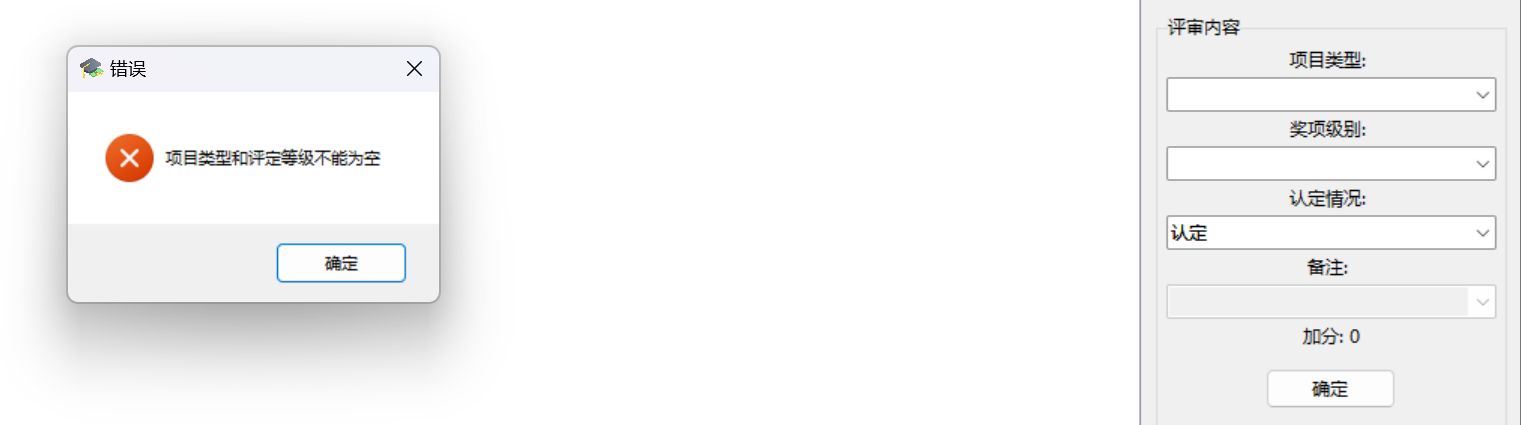
\includegraphics[width=0.7\linewidth]{fig/仅认定确定的提醒}
		\caption{“项目类型”和“奖项级别”不能为空提醒}
		\label{fig:“项目类型”和“奖项级别”不能为空提醒}
	\end{figure}
	
	当“确定”完成某一加分项目后，如果为“不予认定”，该项目“加分”列则为0，并非根据其所属的“项目类型”和“奖项级别”进行加分，如图\ref{fig:不予认定加分为0}所示。
	
	\begin{figure}[H]
		\centering
		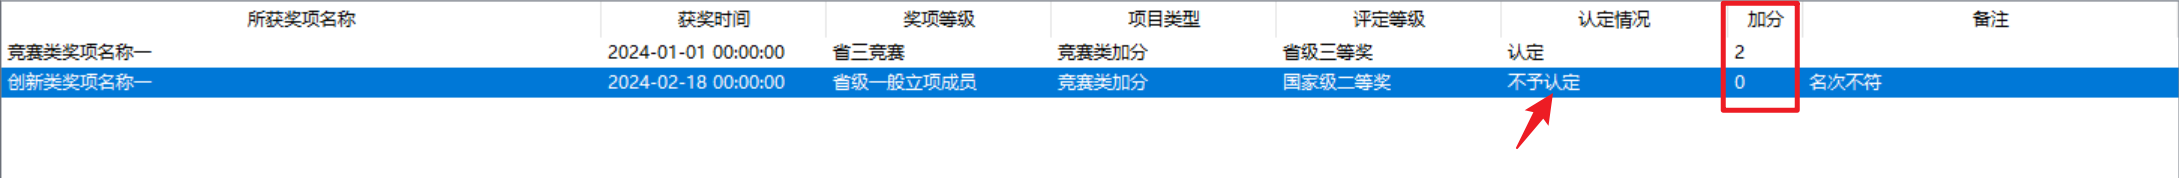
\includegraphics[width=1\linewidth]{fig/不予认定加分为0}
		\caption{不予认定的加分项目加分为0}
		\label{fig:不予认定加分为0}
	\end{figure}
	
	
	
	\textcolor{mygreen}{
	\section{学生选择下拉菜单}
	如图\ref{fig:版本V3.0学生选择下拉菜单展示}所示，为版本V3.0支持批量导入Excel文件后新增的学生选择下拉菜单，图示为导入了三名学生的材料内容，通过下拉菜单便捷切换不同学生的评审数据，同时智能保存每个学生的评审进度，切换学生时自动保存当前进度，学生信息展示也会进行更新。
}	

	\textcolor{mygreen}{
	请注意，在单个文件导入的情况下，学生选择下拉菜单并不可用，但在补充导入文件后，将从单文件处理状态专户为批量处理状态，此时，学生选择下拉菜单即可正常工作。
	}
	
	\begin{figure}[h]
		\centering
		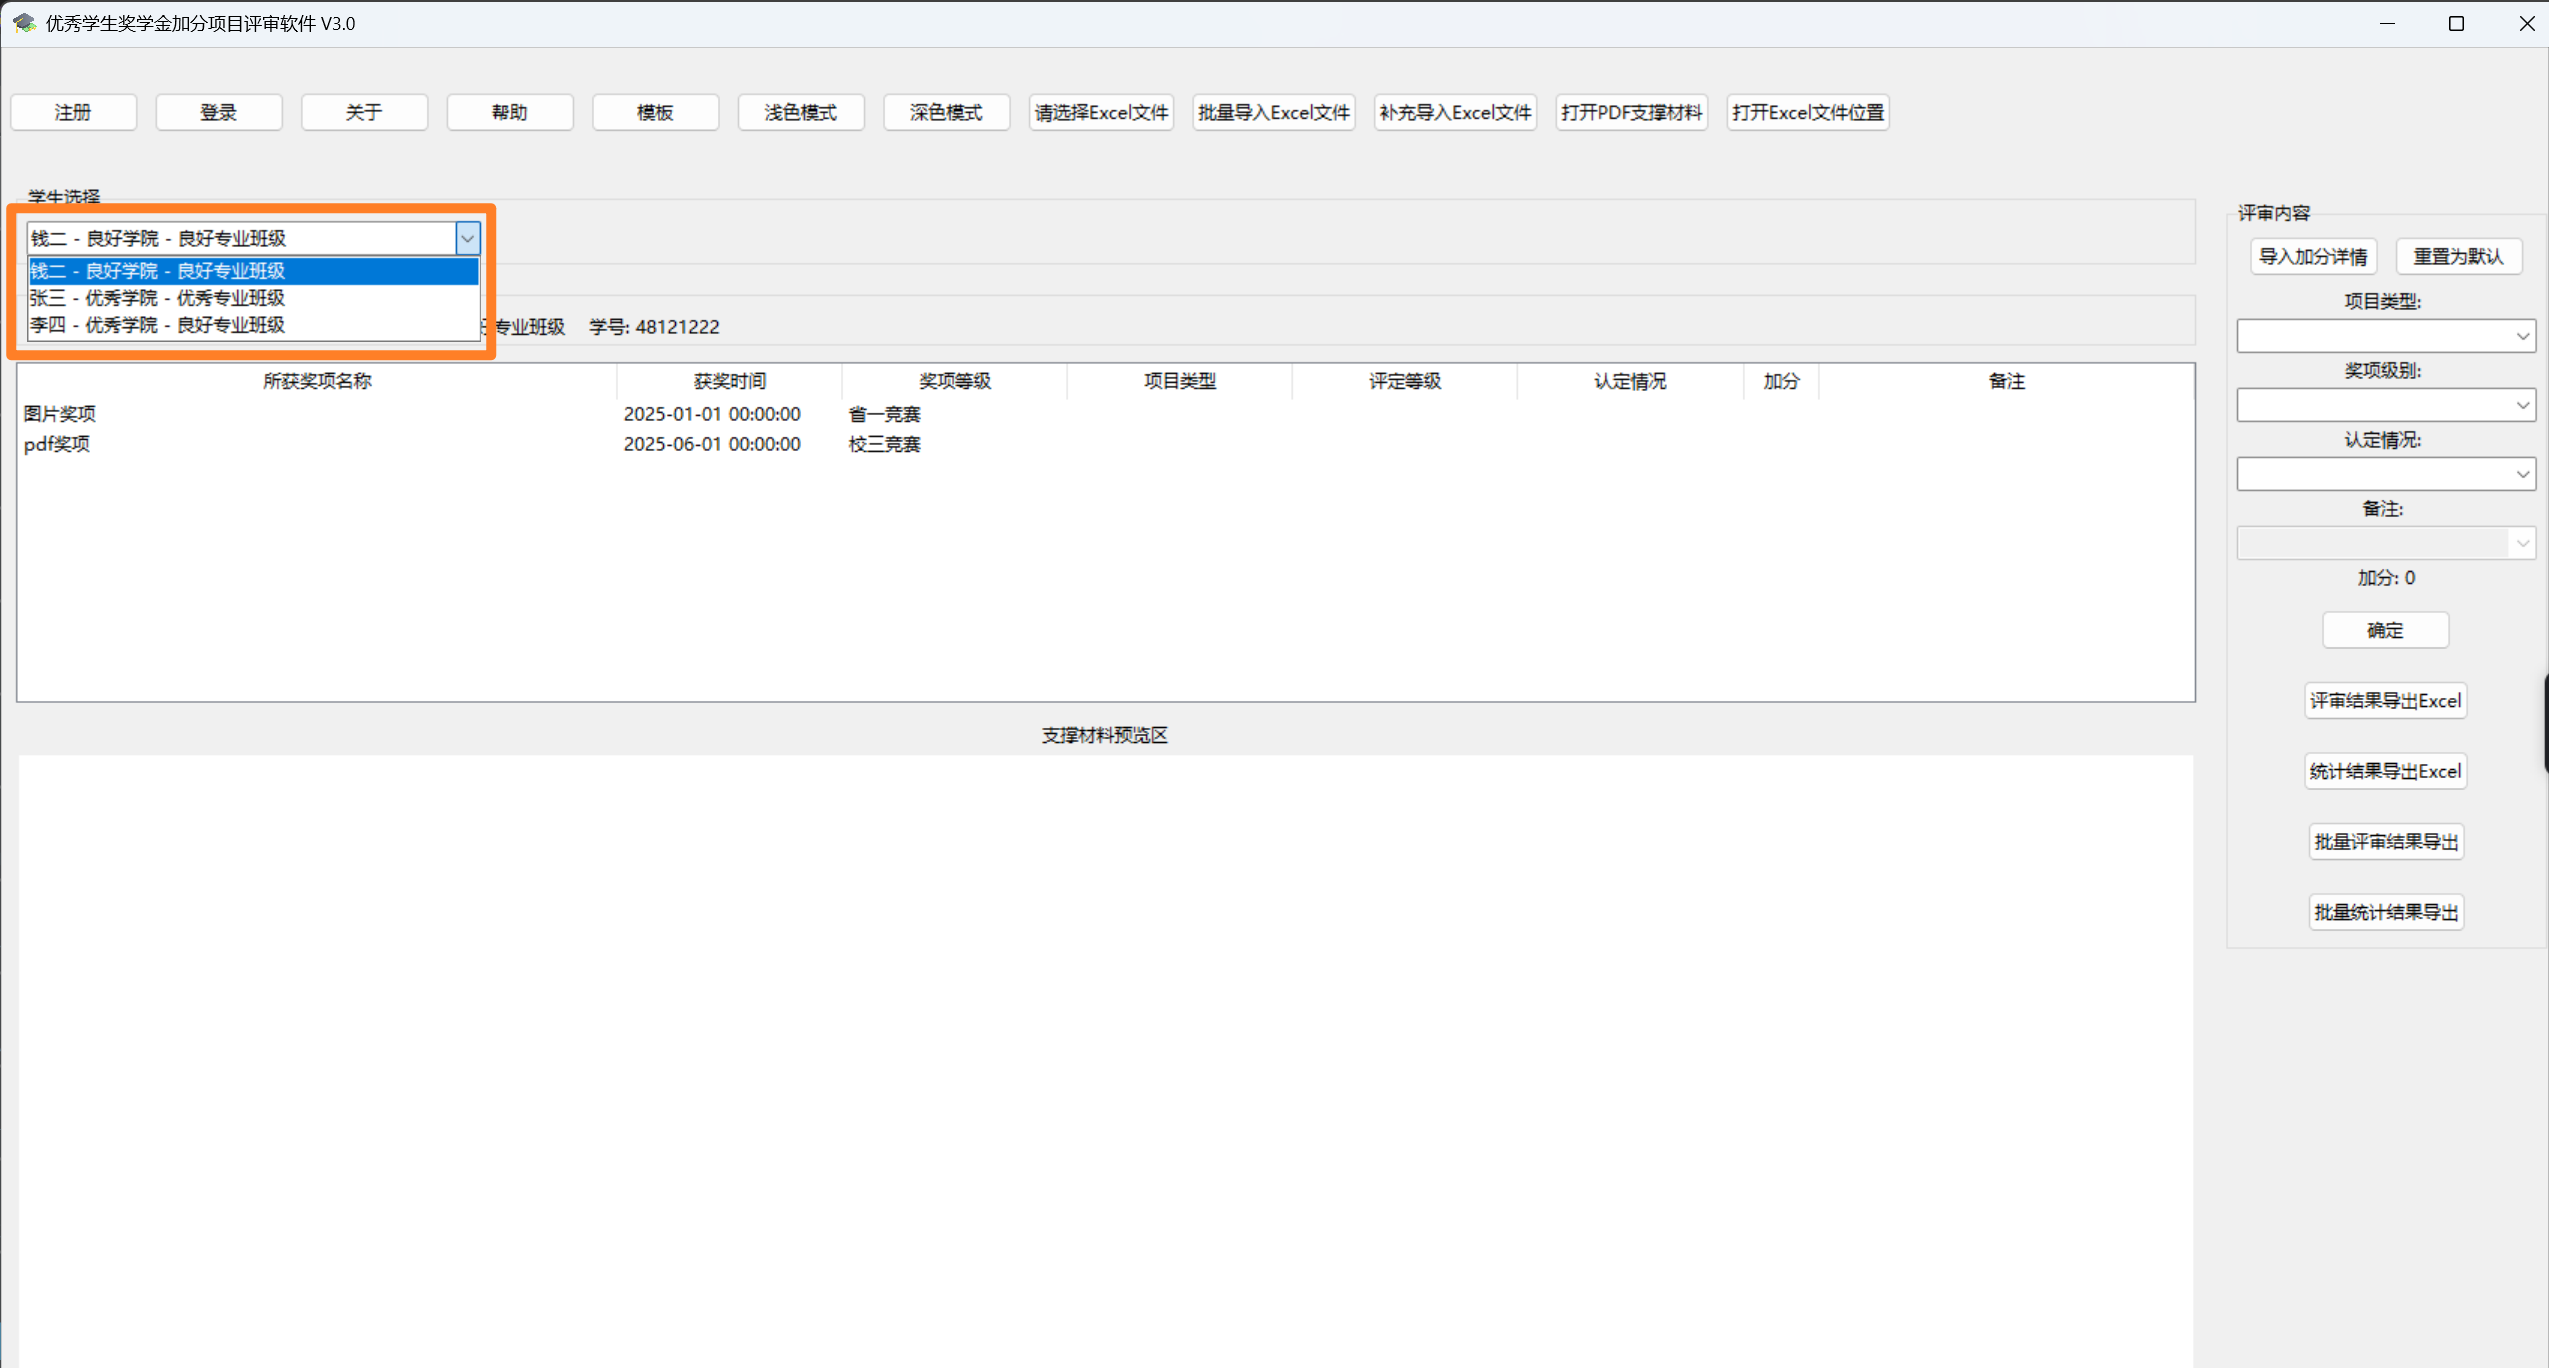
\includegraphics[width=0.7\linewidth]{fig/3.0学生选择下拉菜单}
		\caption{版本V3.0学生选择下拉菜单展示}
		\label{fig:版本V3.0学生选择下拉菜单展示}
	\end{figure}
	
	\section{评审结果导出}
	当所有的加分项目完成评审后，点击“评审结果导出Excel”，会弹窗选择文件保存位置和文件名称，默认文件名称为“学院\_姓名\_年级\_专业\_学号.xlsx”，如图\ref{fig:评审结果导出}所示。如果未选择保存位置，亦会如图\ref{fig:文件路径未选择提醒}弹窗提示用户。
\begin{figure}[H]
	\centering
	\begin{minipage}{0.5\linewidth}
		\centering
		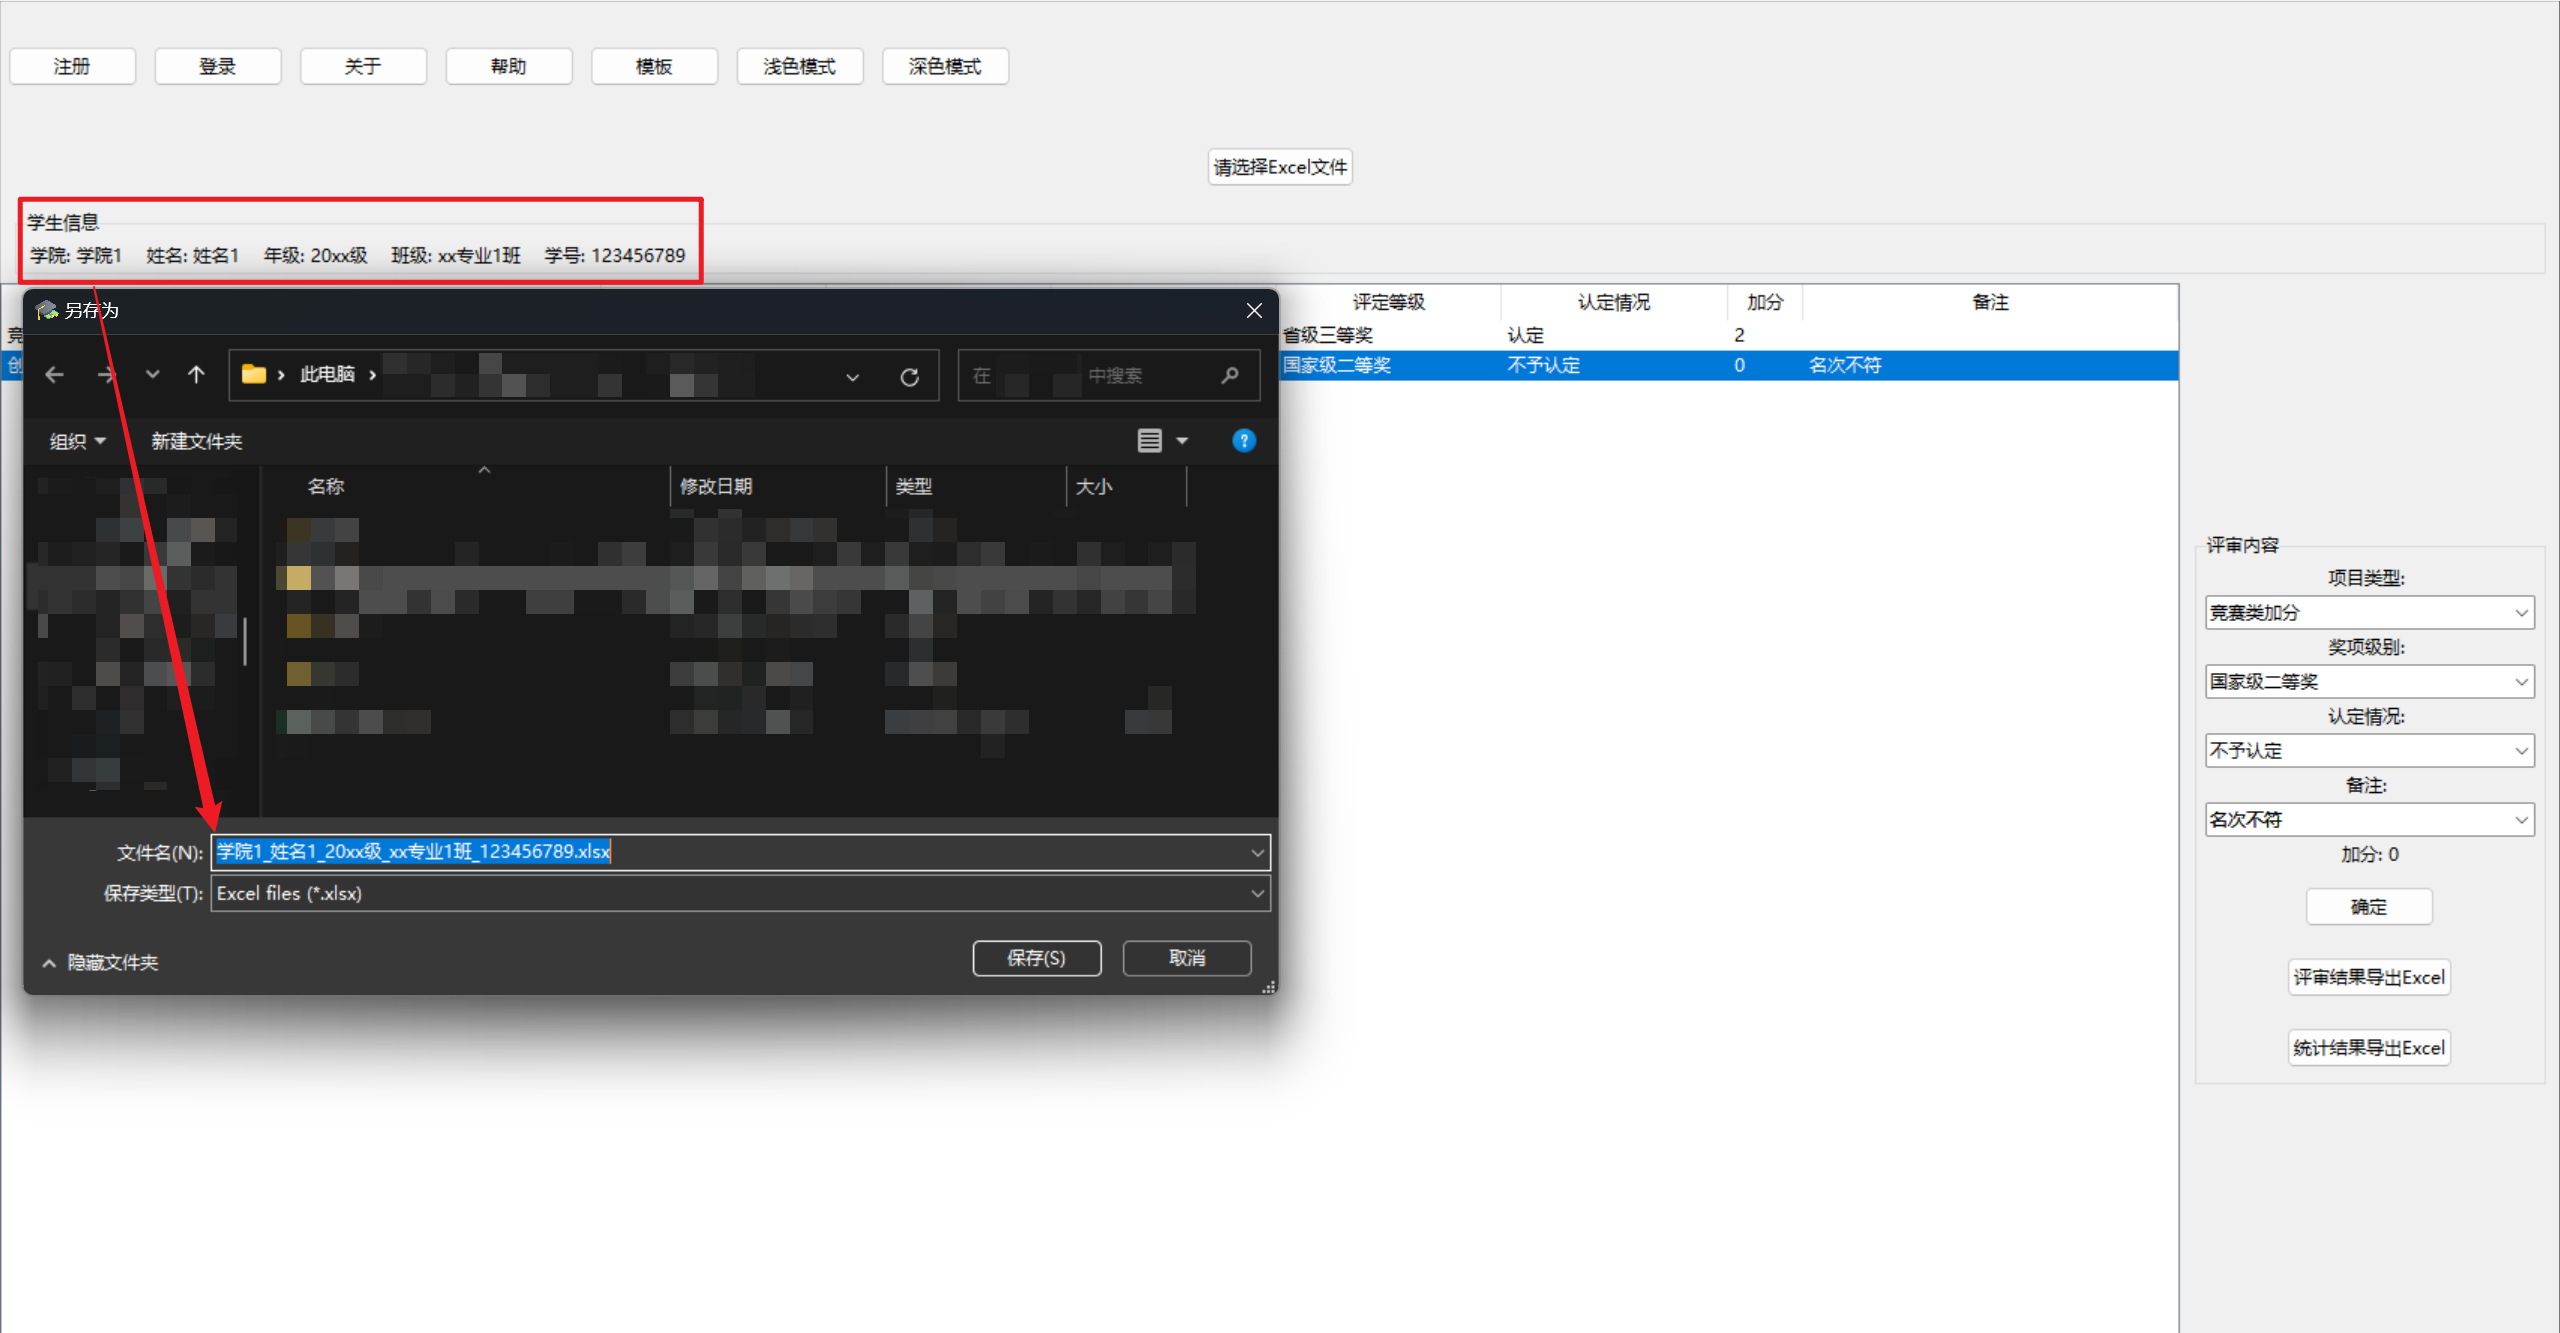
\includegraphics[width=\linewidth]{fig/评审结果导出文件位置选择}
		\caption{评审结果导出}
		\label{fig:评审结果导出}
	\end{minipage}%
	\hspace{0.02\linewidth}  % 调整两幅图之间的间距
	\begin{minipage}{0.4\linewidth}
		\centering
		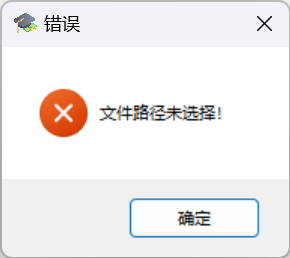
\includegraphics[width=0.7\linewidth]{fig/文件路径未选择}
		\caption{文件路径未选择提醒}
		\label{fig:文件路径未选择提醒}
	\end{minipage}
\end{figure}

	成功导出后会如图\ref{fig:评审结果成功导出提醒}所示弹窗提示用户已成功导出文件，并给出文件保存位置，以备不时之需。
	\begin{figure}[H]
		\centering
		
\includegraphics[width=0.7\linewidth]{fig/导出成功提醒}
		\caption{评审结果成功导出提醒}
		\label{fig:评审结果成功导出提醒}
	\end{figure}
	
	导出的文件的信息如图\ref{fig:评审结果导出文件的示例}所示，包括学院，姓名，年级，班级，学号，所获奖项名称，获奖时间，奖项等级，项目类型，评定等级，认定情况，加分，备注等所有信息。
	
	\begin{figure}[H]
		\centering
		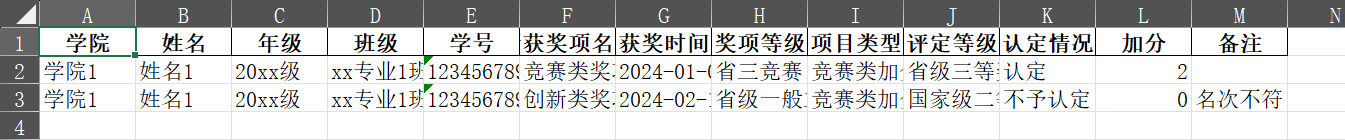
\includegraphics[width=1\linewidth]{fig/评审结果}
		\caption{评审结果导出文件的示例}
		\label{fig:评审结果导出文件的示例}
	\end{figure}
	
	
	\textcolor{mygreen}{
	\section{批量评审结果导出}
	版本V3.0更新中，新支持了批量处理操作，为了适配新功能，对于评审结果的导出，本软件也对应新增了“批量评审结果导出”功能按钮，支持对批量评审的结果进行输出。在点击【批量评审结果导出】后，选择文件导出地址后，输出结果如图\ref{fig:版本V3.0批量评审结果导出}所示，将在选定地址中输出每位学生递交的材料的结果文件和全部学生评审结果总表，其中单个结果内容与单文件评审结果一致，即如图\ref{fig:评审结果导出文件的示例}，全部学生评审结果总表内容如图\ref{fig:版本V3.0批量评审结果导出总表示例}所示。}	
	\begin{figure}
		\centering
		
\includegraphics[width=0.7\linewidth]{fig/3.0批量评审结果导出}
		\caption{版本V3.0批量评审结果导出}
		\label{fig:版本V3.0批量评审结果导出}
	\end{figure}

	\begin{figure}
		\centering
		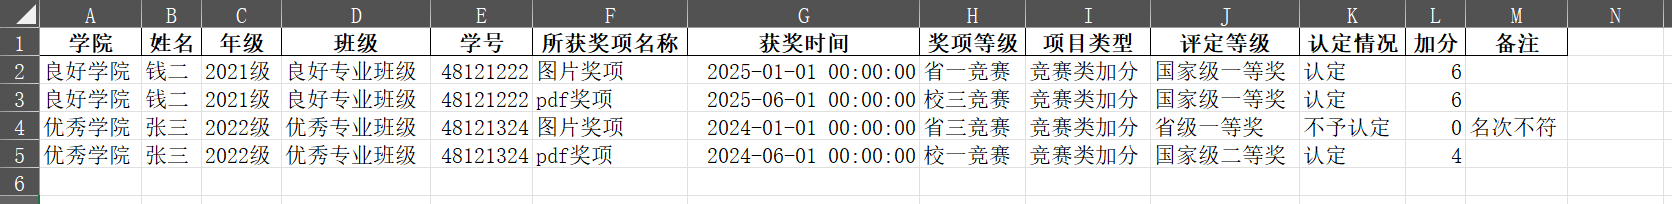
\includegraphics[width=0.7\linewidth]{fig/3.0批量评审结果导出总表}
		\caption{版本V3.0批量评审结果导出总表示例}
		\label{fig:版本V3.0批量评审结果导出总表示例}
	\end{figure}
	
	
	\textcolor{mygreen}{	
	若采用自定义加分规则，则对应的项目类型和奖项级别均按照新的导入加分详情进行输出，如图\ref{fig:版本V3.0自定义加分批量评审结果导出总表示例}所示。
	\begin{figure}[h]
		\centering
		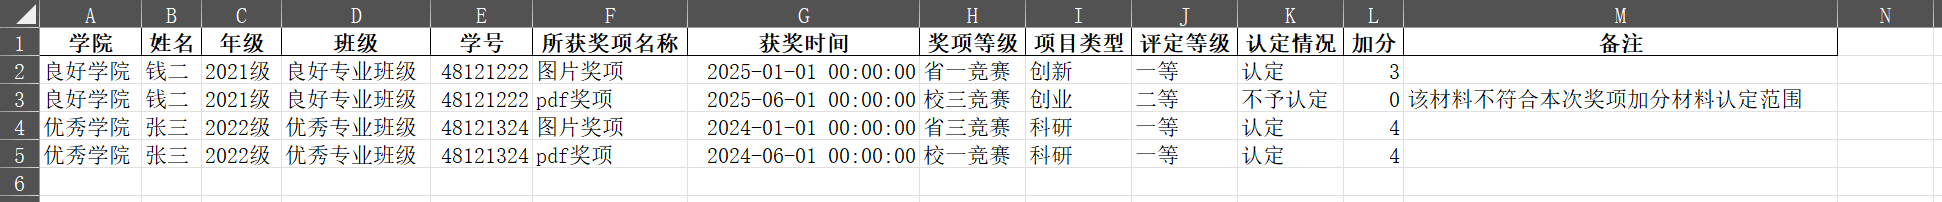
\includegraphics[width=0.7\linewidth]{fig/3.0自定义加分批量评审结果导出总表}
		\caption{版本V3.0自定义加分批量评审结果导出总表示例}
		\label{fig:版本V3.0自定义加分批量评审结果导出总表示例}
	\end{figure}
}	
	
	
	
	
	\section{统计结果导出}
	当所有的加分项目完成评审后，点击“评审结果导出Excel”，会弹窗选择文件保存位置和文件名称，默认文件名称为“学院\_姓名\_年级\_专业\_学号\_统计.xlsx”，如图\ref{fig:统计结果导出}所示。如果未选择保存位置，亦会如图\ref{fig:文件路径未选择提醒1}弹窗提示用户。
\begin{figure}[H]
	\centering
	\begin{minipage}{0.5\linewidth}
		\centering
		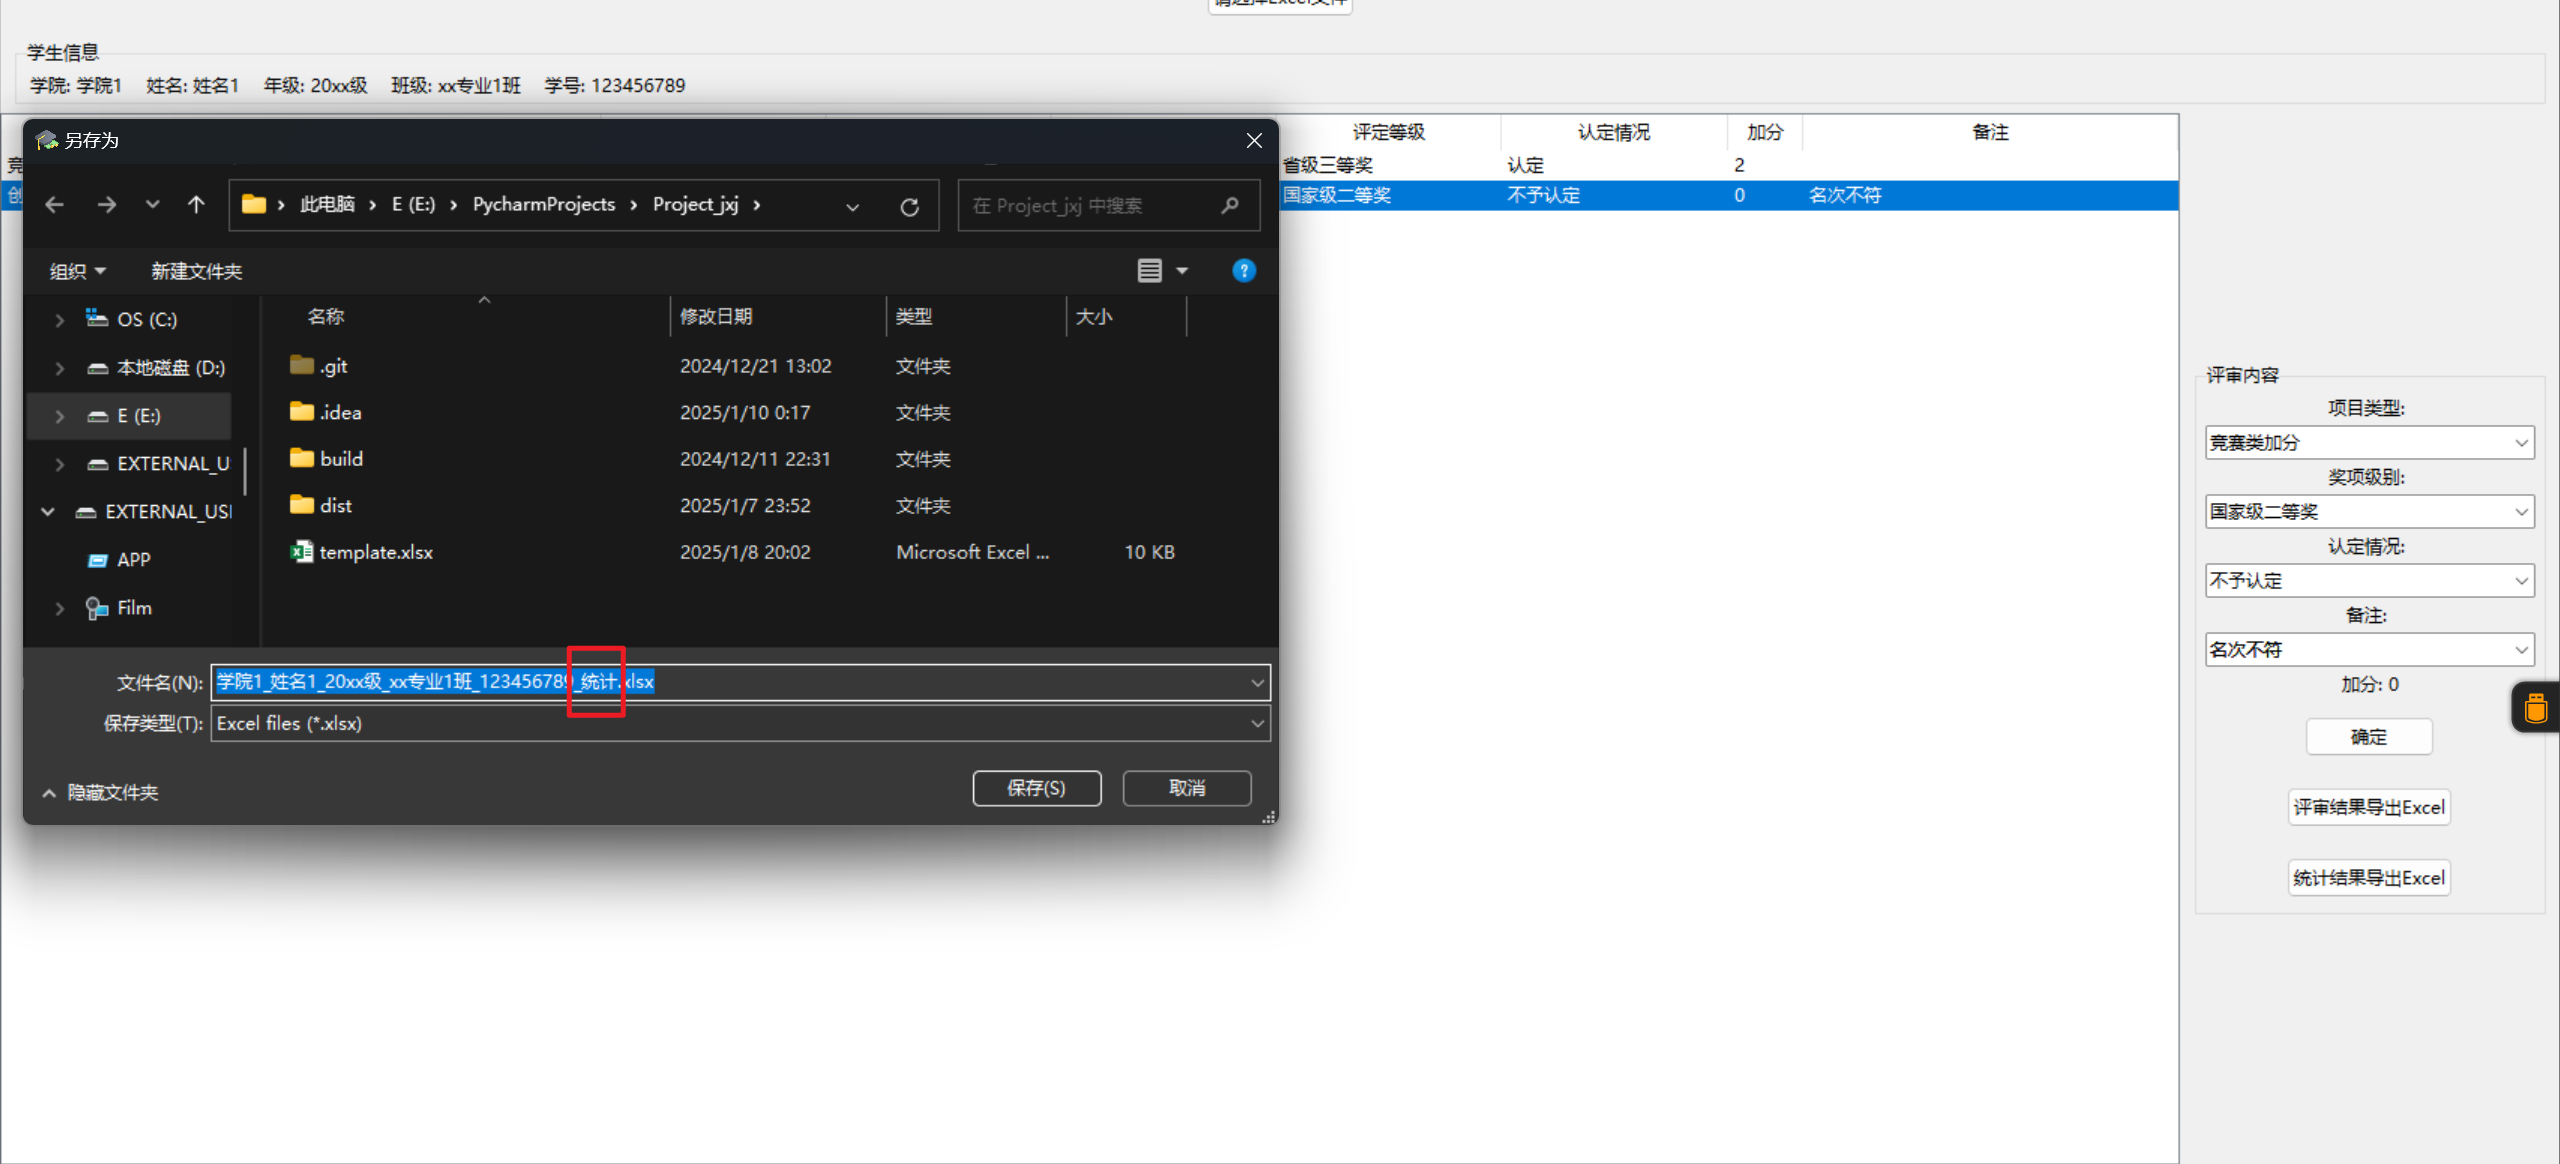
\includegraphics[width=\linewidth]{fig/统计结果导出}
	\caption{统计结果导出}
\label{fig:统计结果导出}
	\end{minipage}%
	\hspace{0.02\linewidth}  % 调整两幅图之间的间距
	\begin{minipage}{0.4\linewidth}
		\centering
		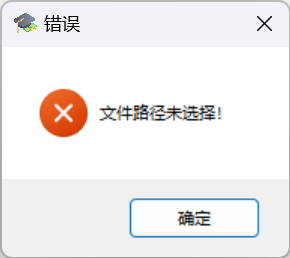
\includegraphics[width=0.7\linewidth]{fig/文件路径未选择}
		\caption{文件路径未选择提醒}
		\label{fig:文件路径未选择提醒1}
	\end{minipage}
\end{figure}

	成功导出后会如图\ref{fig:统计结果成功导出提醒}所示弹窗提示用户已成功导出文件，并给出文件保存位置。
\begin{figure}[H]
	\centering
	
\includegraphics[width=0.7\linewidth]{fig/导出成功2}
	\caption{统计结果成功导出提醒}
	\label{fig:统计结果成功导出提醒}
\end{figure}

导出的文件的信息如图\ref{fig:统计结果导出文件的示例}所示，包括学院，姓名，年级，班级，学号，竞赛类加分，科研创新类加分，外语类加分等所有信息。请注意，软件设置了每种项目类型的加分上限为6分。

\begin{figure}[H]
	\centering
	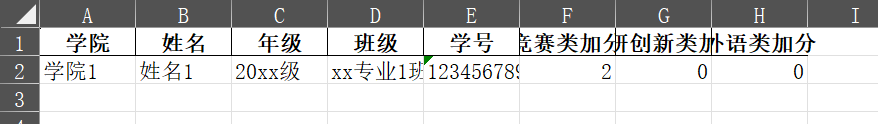
\includegraphics[width=1\linewidth]{fig/统计结果}
	\caption{统计结果导出文件的示例}
	\label{fig:统计结果导出文件的示例}
\end{figure}

	\textcolor{mygreen}{
	\section{批量统计结果导出}
	版本V3.0更新中，新支持了批量处理操作，为了适配新功能，对于统计结果的导出，本软件也对应新增了“批量统计结果导出”功能按钮，支持对批量评审的统计结果进行输出。在点击【批量统计结果导出】后，选择文件导出地址后，输出结果内容如图\ref{fig:版本V3.0统计结果导出示例（默认加分规则）} 所示。}	

	\begin{figure}[h]
		\centering
		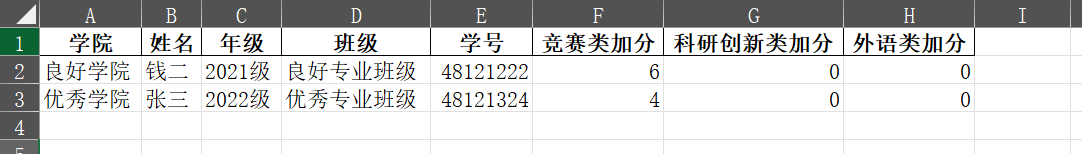
\includegraphics[width=0.7\linewidth]{fig/3.0统计结果导出示例（默认加分规则）}
		\caption{版本V3.0统计结果导出示例（默认加分规则）}
		\label{fig:版本V3.0统计结果导出示例（默认加分规则）}
	\end{figure}

	\textcolor{mygreen}{	
	若采用自定义加分规则，则对应的项目类型和奖项级别均按照新的导入加分详情进行输出，如图\ref{fig:版本V3.0自定义加分批量统计结果导出示例}所示。
	\begin{figure}[h]
		\centering
		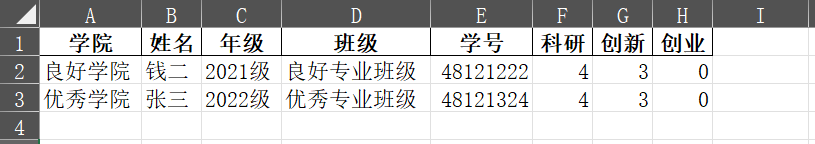
\includegraphics[width=0.7\linewidth]{fig/3.0自定义加分批量统计结果导出示例}
		\caption{版本V3.0自定义加分批量统计结果导出示例}
		\label{fig:版本V3.0自定义加分批量统计结果导出示例}
	\end{figure}
}	

	\section{结果导出保护}
	如图\ref{fig:评审未完成时结果导出提醒}所示，当用户未正确评审完所有的加分项目却选择结果导出时，会弹窗提醒用户还有未完成的评审项目。
	\begin{figure}[H]
		\centering
		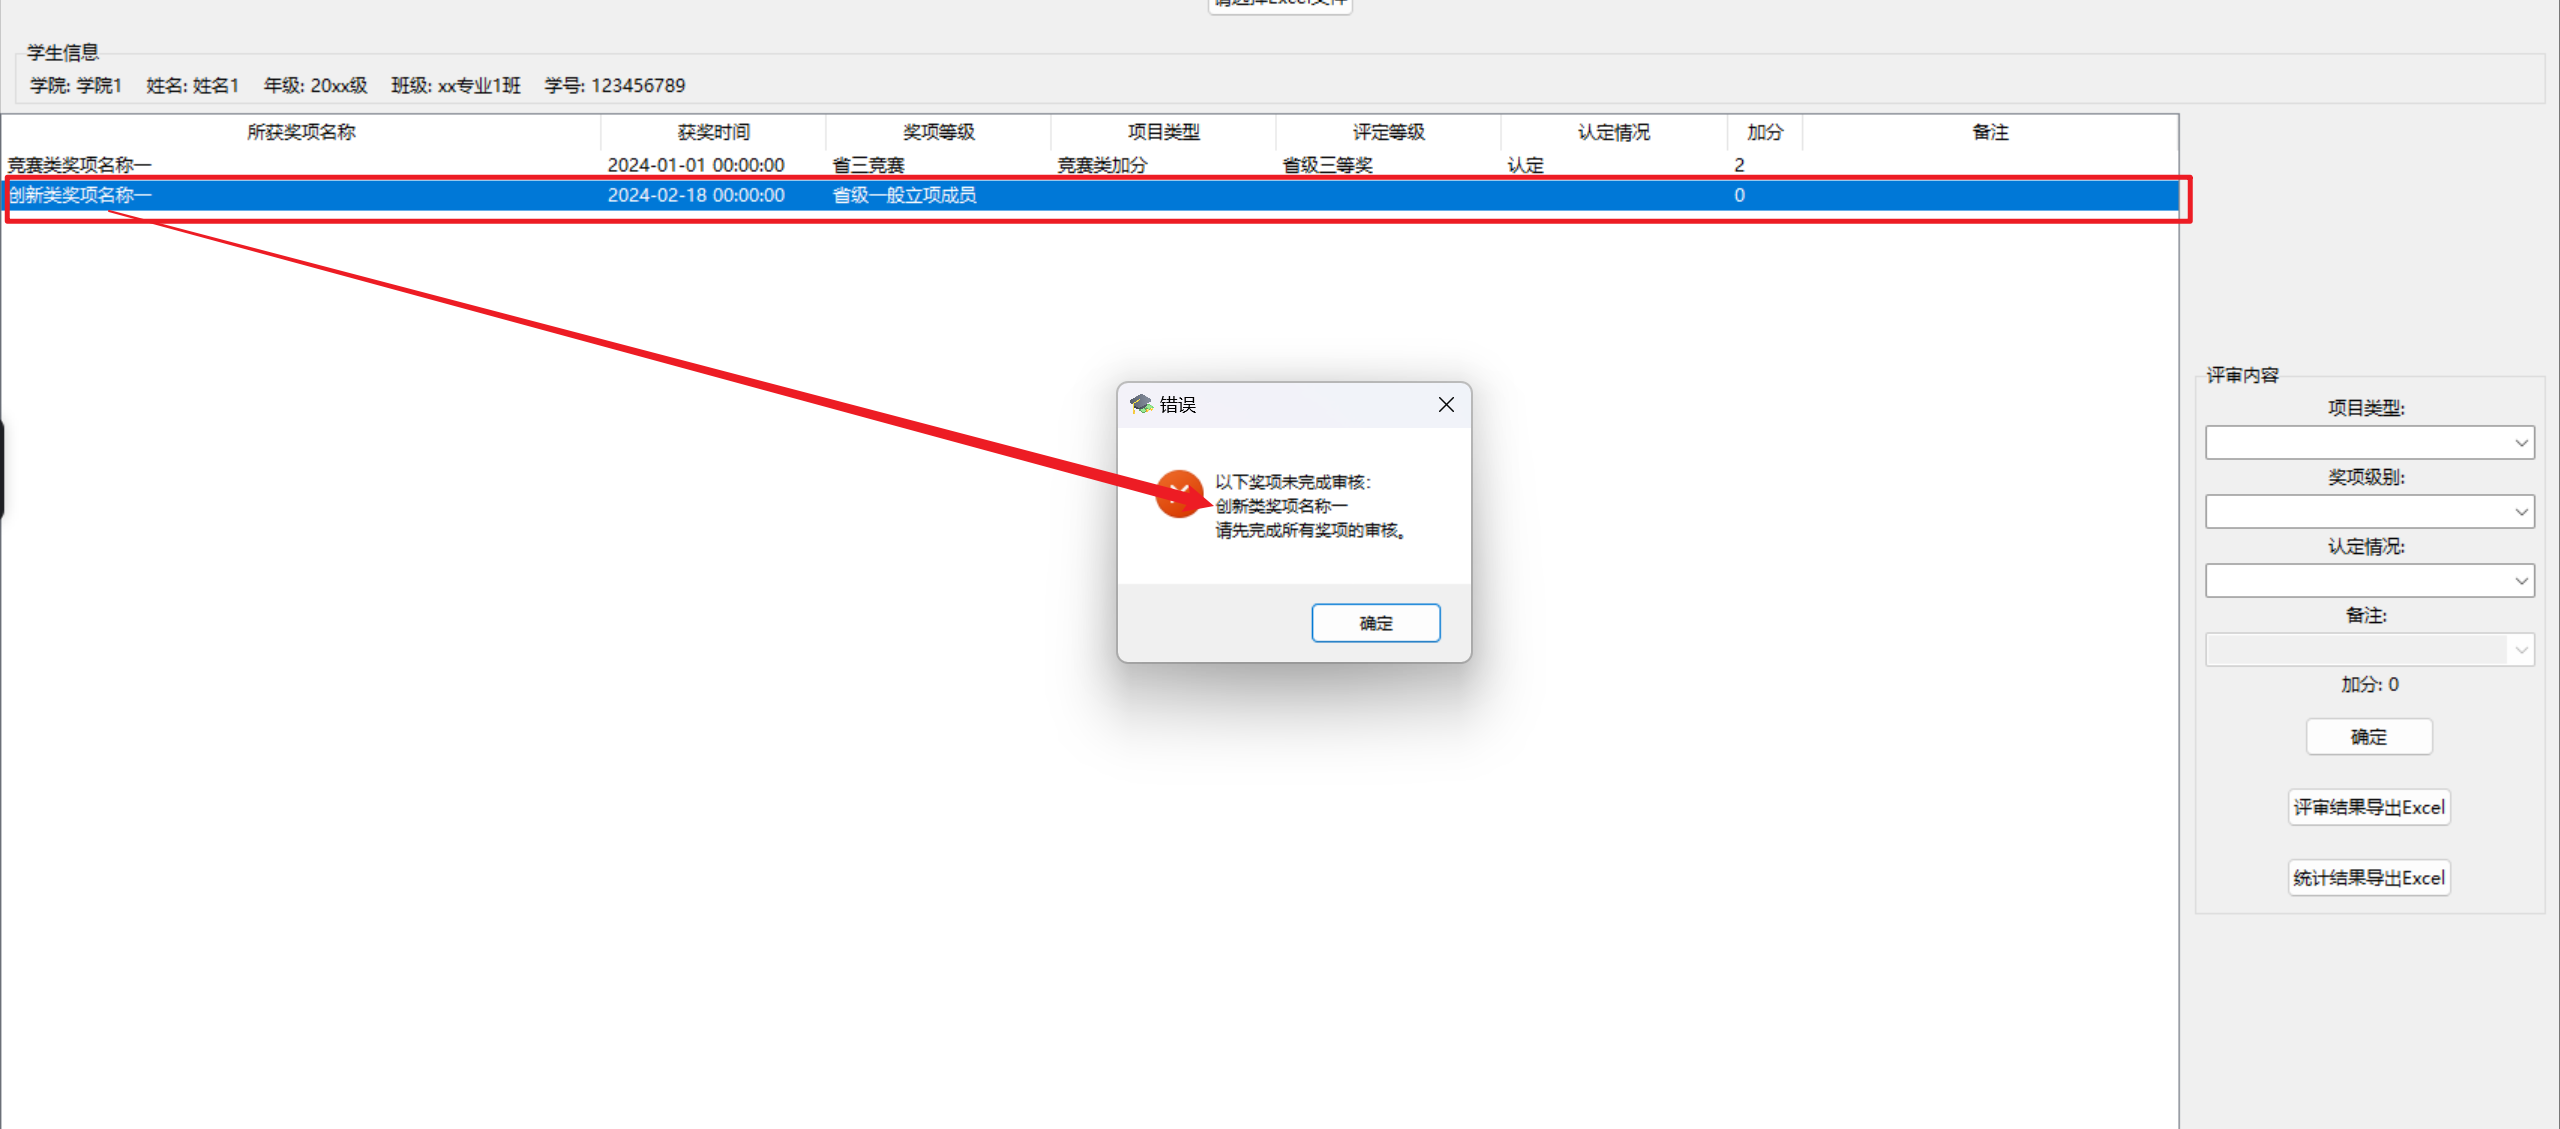
\includegraphics[width=0.7\linewidth]{fig/评审未完成时结果导出提醒}
		\caption{评审未完成时结果导出提醒}
		\label{fig:评审未完成时结果导出提醒}
	\end{figure}
	
	\textcolor{mygreen}{
		如图\ref{fig:版本V3.0未完成批量评审而导出的弹窗提醒}所示，在批量处理状态，如果没有完成所有学生的评审工作而进行结果导出，则会进行提醒，避免评审人员出现工作疏漏的情况。
	\begin{figure}[h]
		\centering
		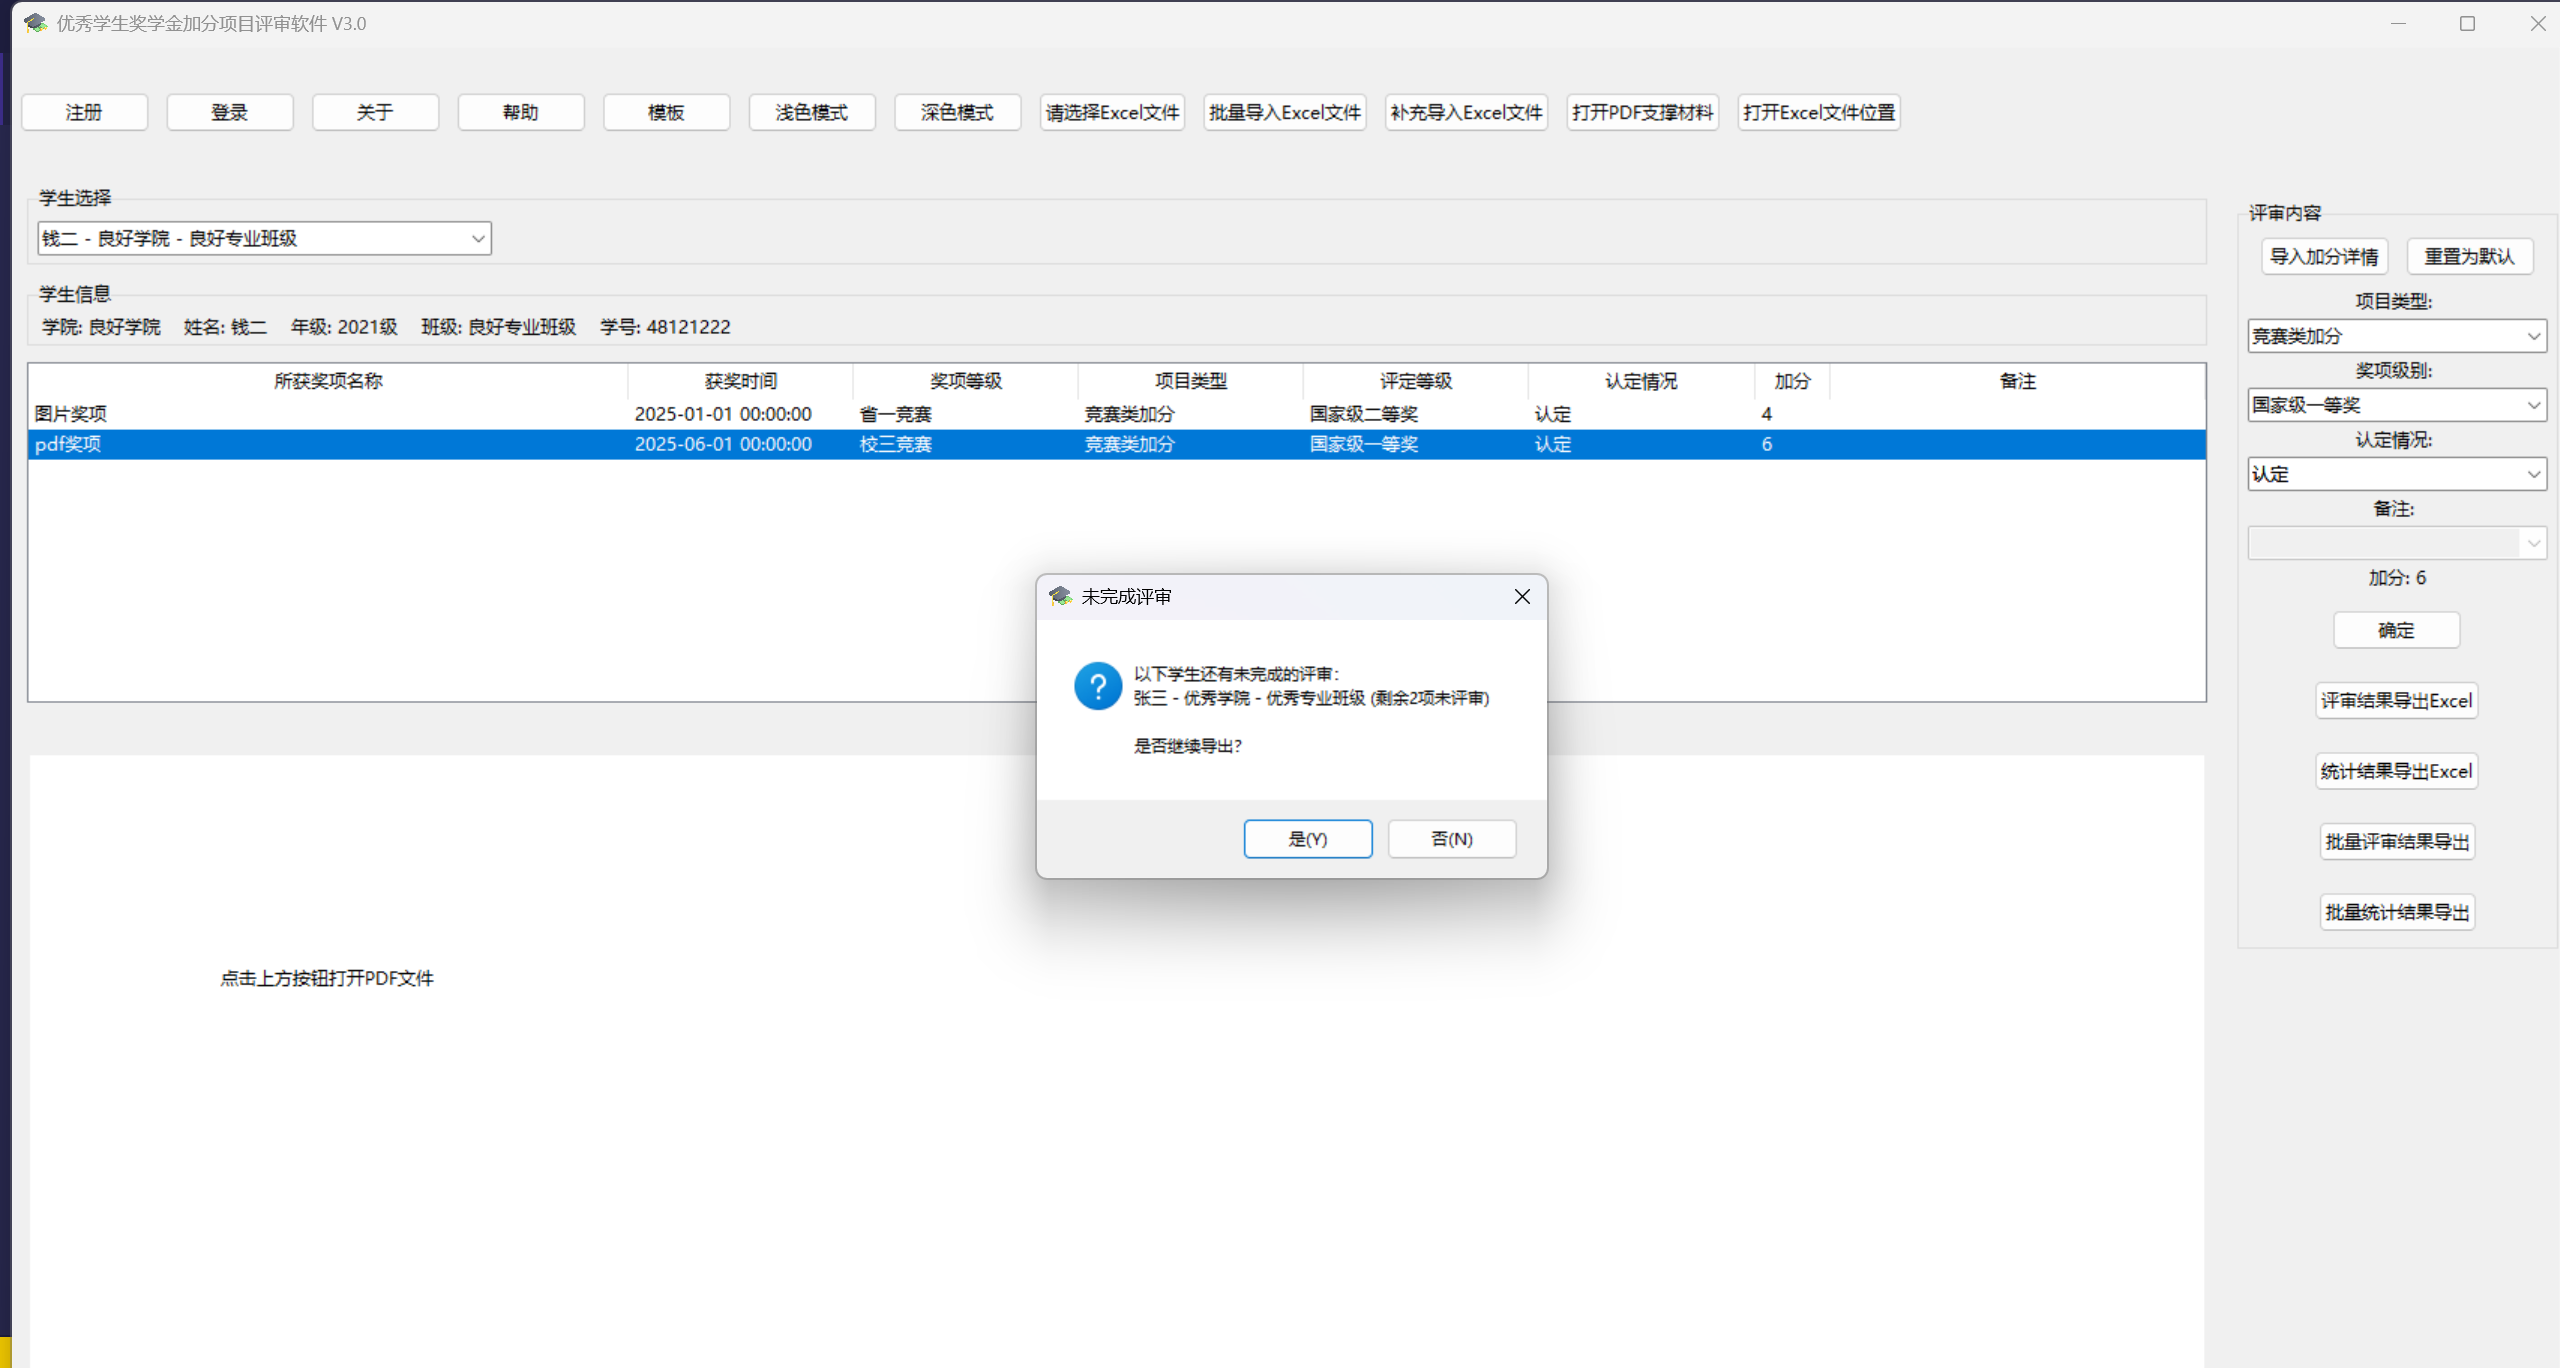
\includegraphics[width=0.7\linewidth]{fig/3.0未完成批量评审而导出的弹窗提醒}
		\caption{版本V3.0未完成批量评审而导出的弹窗提醒}
		\label{fig:版本V3.0未完成批量评审而导出的弹窗提醒}
	\end{figure}
	}
	
	
	\section{意外退出保护}
	如图\ref{fig:意外退出保护提醒}所示，当导入文件后，如果用户不小心点击关闭软件，会弹窗提醒用户还有未导出的评审结果，二次确定是否需要关闭软件。请注意，在提醒后仍选择确定关闭软件将不保存已评审的内容！若用户已导出评审结果或统计结果，将不在意外退出保护的范围内！
	\begin{figure}[H]
		\centering
		
\includegraphics[width=0.7\linewidth]{fig/意外退出保护提醒}
		\caption{意外退出保护提醒}
		\label{fig:意外退出保护提醒}
	\end{figure}
	 
	 
	 \textcolor{myred}{
		\section{打开EXCEL文件位置}
		此操作将打开读取的EXCEL文件所在的目录，可以帮助评审人员快速查看文件所在目录和递交的材料，减轻负担。
	} 
	
	\textcolor{mygreen}{
		\section{导入加分详情及重置为默认}
		【导入加分详情】将采用自定义加分规则更新评审内容选项（项目类型、奖项级别、加分和加分上限）。
	}
	
	\textcolor{mygreen}{
		【重置为默认】将更新评审内容选项为默认规则，如表\ref{分值表}所示。
	} 
	
	\chapter{总结与展望}
	\section{总结}
	本软件旨在通过自动化和简化的方式提高奖学金评审的效率，减少人为错误，并确保评审过程的公正性和高效性。系统设计涵盖了从启动、界面操作到评审流程的各个环节，具体包括：
	
\begin{itemize}
	\item 	项目背景：阐述了优秀学生奖学金评审的必要性，并强调了该软件在简化评审流程、提高工作效率方面的重要作用。
	\item 	编写目的：为软件使用者提供详细的操作指南，确保软件能够得到有效使用。
	\item 	适用范围与对象：明确了使用对象为高校评审委员会及相关工作人员，并列举了适用场景，如奖学金评审、学术竞赛评定等。
	\item 	软件概述与界面介绍：展示了软件的启动方式、主界面设计、操作按钮功能等，用户可以通过简单的操作完成学生信息和加分项目的评审。
	\item 	软件操作教程：详细介绍了软件的基本使用流程，涵盖加分项目的数据收集、信息填写、注册与登录操作等。
\end{itemize}
	\section{展望}
	随着软件版本的更新，以下是未来可能的改进方向：
	
\begin{enumerate}
	\item 	功能扩展：增加更高级的统计分析功能，如自动生成评审报告、历史数据对比等。
	\item 	界面优化：虽然现有界面已简洁易用，未来可进一步优化界面布局、增加更多自定义选项，提升用户体验。
	\item 	智能化评审：引入人工智能技术，自动识别学生的综合素质评分，减少人工评审的主观性和误差。
	\item 	跨平台支持：目前软件支持Windows系统，未来可以扩展至Mac和Linux平台，增加更多的操作系统兼容性。
\end{enumerate}

	\chapter{附录}
	考虑到使用说明书的排版美观，本章节用于放置可能出现的长篇幅表格/图像内容（不宜在正文中进行展示或正文中展示排版困难或不美观），可通过点击下行列表中进行快速跳转。
	
	\begin{enumerate}
		\item \hyperref[分值表]{加分项目分值表}
	\end{enumerate}
	
	
	\begin{table}[htbp]
	\centering
	\small
	\renewcommand{\arraystretch}{1} % 调整缩短行间距
	\caption{加分项目分值表}
	\begin{tabular}{cccccc}
		\toprule%第一道横线 
		\textbf{竞赛类加分} & \textbf{加分} & \textbf{科研创新类加分} & \textbf{加分} & \textbf{外语类加分} & \textbf{加分} \\  \midrule%第二道横线            
		国家级一等奖 & 6 & 国家级立项主持人 & 6 & 大学英语四级（CET4） & 1 \\ 
		国家级二等奖 & 4 & 国家级立项学生成员 & 4 & 英语专业四级（TEM4） & 1 \\ 
		国家级三等奖 & 3 & 省级重点立项主持人 & 5 & 雅思（IELTS） & 2 \\ 
		省级一等奖 & 5 & 省级重点立项学生成员 & 3 & 托福（TOEFL） & 2 \\ 
		省级二等奖 & 3 & 省级一般立项主持人 & 3 & 剑桥英语考试 & 2 \\ 
		省级三等奖 & 2 & 省级一般立项学生成员 & 2 & 培生英语考试 & 2 \\
		市级一等奖 & 3 & 校级立项主持人 & 2 & GRE & 2 \\ 
		市级二等奖 & 2 & 校级立项学生成员 & 1 & GMAT & 2 \\ 
		市级三等奖 & 1 & SCI论文一作 & 6 & 其他符合外语类加分项目（2分） & 2 \\
		校级一等奖 & 2 & SCI论文二作 & 4 & 其他符合外语类加分项目（1分） & 1 \\
		校级二等奖 & 1 & SCI论文三作 & 3 & 大学英语六级（CET6） & 2 \\ 
		校级三等奖 & 0.5 & 核心期刊论文一作 & 3 & 英语专业八级（TEM8） & 2 \\ 
		院级一等奖 & 1 & 核心期刊论文二作 & 2 & & \\ 
		院级二等奖 & 0.5 & 核心期刊论文三作 & 1 & & \\ 
		院级三等奖 & 0.3 & 普通期刊论文一作 & 2 & & \\ 
		& & 普通期刊论文二作 & 1 & & \\ 
		& & 普通期刊论文三作 & 0.5 & & \\ 
		& & 版权著作 & 1 & & \\ 
		& & 发明专利一作 & 6 & & \\ 
		& & 发明专利二作 & 4 & & \\ 
		& & 发明专利三作 & 3 & & \\ 
		& & 实用新型专利一作 & 2 & & \\ 
		& & 实用新型专利二作 & 1 & & \\ 
		& & 实用新型专利三作 & 0.5 & & \\ 
		& & 外观专利一作 & 2 & & \\ 
		& & 外观专利二作 & 1 & & \\ 
		& & 外观专利三作 & 0.5 & & \\ 
		\bottomrule%第三道横线
	\end{tabular}
	\label{分值表}
\end{table}

\end{document}
